\documentclass[12pt,a4paper]{ctexart}%A4纸张,ctexart为文章类型,改格式支持中文
%\usepackage[top=30mm,bottom=25mm,left=25mm,right=25mm]{geometry}%页面布局
\usepackage[top=2cm,bottom=3cm,left=3cm,right=3cm,includehead,includefoot]{geometry} %文档排版结构设置
\usepackage{graphicx}%图片载入
\usepackage{float}%图片浮动环境,类似于word中的文字浮动和图片的关系
\usepackage{amsmath}%数学环境
%\usepackage{epstopdf}% eps格式图片使用宏包
\usepackage{pdfpages}   % 直接插入pdf的宏包
\usepackage{ulem}
%\usepackage{url}%超链接
%\usepackage{identfirst}
\usepackage{setspace}%行间距设置宏包
%\usepackage{marginnote}% 边注宏包
%\usepackage{subfigure}
%\usepackage{subfig}
%\usepackage{diagbox}
%\usepackage{appendix}%增加附录
\usepackage{fancyhdr}% 设置页眉和页脚宏包
%\usepackage{xcolor}% 边框设置宏包
%\usepackage{listings}% 边框样式设置
\usepackage{titlesec}% 标题与段落间距
\usepackage{titletoc} % 目录设置
\usepackage{xeCJK} %字体设置
%\usepackage[numbers,compress]{natbib} % 文献引用设置
\usepackage[colorlinks,linkcolor=blue,anchorcolor=blue,citecolor=blue]{hyperref}  % 公式,文献引用设置超链接
\usepackage{cite} % 参考文献引用设置




%宏包导入
\linespread{1.6}%行间距设置
\numberwithin{equation}{section}%公式按照章节标号
\renewcommand\thefigure{\thesection.\arabic{figure}}%图片按章节标号
\makeatletter
\@addtoreset{figure}{section}
\renewcommand{\figurename}{图}               % 对图表中的Fig进行中文翻译变为图
\renewcommand{\contentsname}{目录}           % 对Contents进行汉化为目录
\renewcommand\listfigurename{插\ 图\ 目\ 录} % 对List of Figures进行汉化为插图目录
\renewcommand\listtablename{表\ 格\ 目\ 录}  % 对List of Tables进行汉化表格目录
\setcounter{tocdepth}{2}%目录章节深度设置

%\setlength{\parskip}{0.5\baselineskip}% 设置空行换行后,上下两段文字间距
%\titlespacing*{section}{0pt}{9pt}{0pt}% 设置标题与段落间距
%============================= 目录设置 ======================
\titlecontents{chapter}[1.5em]{\zihao{3}\bf }{\contentslabel{1.5em}}{\hspace*{-2em}}{\titlerule*[5pt]{$\cdot$}\contentspage}
\titlecontents{section}[3.3em]{\zihao{-3}\bf }{\contentslabel{1.8em}}{\hspace*{-2.3em}}{\titlerule*[5pt]{$\cdot$}\contentspage}
\titlecontents{subsection}[2.5em]{\zihao{3}}{\thecontentslabel{$\quad$}}{}{\titlerule*[5pt]{$\cdot$}\contentspage}

%=================================================================================
\renewcommand{\baselinestretch}{2.0} %行间距1.5倍
%===============================页眉页脚设置================================
\fancypagestyle{plain}{
%\fancyhead[RE]{\leftmark} % 在偶数页的右侧显示章名
\fancyhf{}
%\fancyhead[C]{\rightmark} %页眉居中显示章节名
\fancyhead[C]{高温超导异质结中的旋转对称破缺和部分马约拉纳角态} %页眉居中设置论文标题
\fancyfoot[C]{第\thepage 页}
%\fancyhead[LO]{\rightmark} % 在奇数页的左侧显示小节名
%\fancyhead[LE,RO]{~\thepage~} % 在偶数页的左侧,奇数页的右侧显示页码
% 设置页脚:在每页的右下脚以斜体显示书名
%\fancyfoot[RO,RE]{\it \text{右下角内容}} %右下角增加\text{}中的内容
\renewcommand{\headrulewidth}{1.0pt} % 页眉与正文之间的水平线粗细
\renewcommand{\footrulewidth}{1.0pt}
%\renewcommand{\footrulewidth}{0pt}
%\renewcommand\headrule{\hrule width \hsize height 2pt \kern 2pt \hrule width \hsize height 0.4pt}%页眉上双线
}

%文章整体格式与布局设置
%==================   正文  ======================================
\begin{document}
\songti
%作者信息与论文信息
\clearpage
\author{YuXuan-Li}
\title{硕士毕业论文初稿}
\date{\today}
\maketitle
%毕业论文封面

\includepdf{cover/cover.pdf}

%======================页码设置=====================
% empty - 没有页眉和页脚
% plain - 没有页眉,页脚包含一个居中的页码
% headings - 没有页脚,页眉包含章/节或者字节的名字和页码
% myheadings - 没有页脚,页眉包含有页码
\pagestyle{plain}
\setcounter{page}{1}%当前页为第一页
\pagenumbering{Roman}
% arabic - 阿拉伯数字
% roman - 小写的罗马数字
% Roman - 大写的罗马数字
% alph - 小写的字符形式
% Alph -大写的字符形式
%======================================================================
%\makeatother %生成目录
%\addcontentsline{toc}{chapter}{\contentsname}
%\tableofcontents%增加章节目录

%\newpage%另起一页
%\listoftables%增加表格目录
%=================摘要==================
\newpage
%\setcounter{page}{1} \renewcommand{\thepage}{\wuhao\Roman{page}} % 页码设置
{\centering{\zihao{3}{\bf 高温超导异质结中的旋转对称破缺和部分马约拉纳角态}}\\}
\bigskip
{\zihao{-4}
	\begin{center}
		\begin{tabular}{l}
			专业名称:$\quad$凝聚态物理$\quad\qquad$$\quad\qquad$$\quad$$\quad$$\quad$$\quad$$\quad$$\quad$\\
			申请者: $\quad\quad$李玉轩$\quad\qquad$$\quad\qquad$$\quad\qquad$\\
			导师姓名:$\quad$周涛\quad 教授$\quad\qquad$$\quad\qquad$$\quad\qquad$\\
		\end{tabular}
\end{center}}
\bigskip
\bigskip
\bigskip
{\flushleft{\zihao{-3}\heiti 摘\quad 要}}
\addcontentsline{toc}{section}{摘\quad 要}

%\setlength{\baselineskip}{26pt}
%\thispagestyle{empty}
 近些年来,拓扑绝缘体在理论与实验上都有了非常迅速的发展,由于超导体的配对能隙与绝缘体能隙之间的具有相似性,拓扑超导体同样引起了研究人员的关注。而对于拓扑体系,体边对应是其最主要的特征之一,拓扑超导体的体态虽然是存在电子配对能隙的,但是边界上存在受拓扑保护的边界态,因为超导体中粒子空穴对称性的存在,这个边界态与马约拉纳费米子密切相关,马约拉纳费米子自身也是其反粒子,而且其满足非阿贝尔统计,在拓扑量子计算方面具有非常好的利用潜力。最近研究人员发现了一种新的对应关系体角对应,即对于一个二维的体系,其拓扑保护的边界态出现在比系统低两个维度的角落处,在一个拓扑超导的二维系统中,会出现马约拉纳角态。
 
 以前,基于维象的模型,研究人员提出了可以在二维拓扑绝缘体和高温超导体的异质结系统中实现高阶拓扑超导体,通过将超导电子配对直接加入到拓扑绝缘体哈密顿量中,研究结果显示对于一个四方样品,马约拉纳束缚态会出现在系统的各个角落。本论文中,我们从微观模型出发,我们同时考虑了超导体与二维拓扑绝缘体,并将两者之间的耦合考虑进来,从理论上重新研究了该系统。首先我们计算了谱函数,发现在考虑了耦合之后发现低能下谱函数主要来自于超导体的贡献,而能量较高时由于拓扑绝缘体与超导体之间的耦合,与唯象模型相比能谱发生了较大的变化。接下来从开边界能带图以及实空间中的局与电子态密度结果中,我们发现与唯象模型不同,这里马约拉纳角态并非出现在系统的每一个角落,因为系统中$i_y=N$边界上的边界态并未打开能隙,而其余三个边界上都存在超导诱导出的能隙,所在$i_y=N$这条边界与相邻边界之间不存在反号的质量项,从而无法在相邻边之间的角落处形成角态。我们从动量空间与实空间的序参量计算可知,近邻效应在拓扑绝缘体中诱导出来的电子配对可以同时包含$d$波与$p$波,它们一起作用后会使得某一个边界上的电子配对变得非常小,从而无法将拓扑绝缘体边界态打开能隙,实空间序参量的结果也同样证实了这一点。最后我们利用格林函数运动方程方法求解了动量空间中的反常格林函数,我们发现他可以表示为奇函数与偶函数部分,正对应着数值计算中电子配对的$p$波与$d$波电子配对,解析得到的结果与数值结果完全一致。
 
 通过数值以及理论的分析,我们成功的揭示了通过异质结系统实现利用超导的近邻效应来实现高阶拓扑超导体时,马约拉纳角态并不是在所有的角落中都会出现,这对之后在实验上实现以及观测高阶拓扑超导体中的马约拉纳角态以及利用其实现拓扑量子计算都具有重要的意义。\\
\quad\noindent{\zihao{-4}\heiti 关键词:}高阶拓扑超导,马约拉纳,拓扑绝缘体,准粒子

\newpage
{\centering \zihao{-3}{\heiti Rotational symmetry breaking and partial Majorana corner states in a heterostructure based on high-T$_c$ superconductors}}
\bigskip
{\zihao{-3}
	\begin{center}
		\begin{tabular}{l}
			Major:$\quad\quad$Condensed Matter Physics$\quad\qquad$$\quad\qquad$\\
			Name:$\quad\quad$YuXuan-Li$\quad\qquad$$\quad\qquad$\\
			Supervisor: Tao Zhou$\quad\qquad$\\
		\end{tabular}
\end{center}}
\bigskip
\bigskip
\bigskip

{\flushleft{\zihao{-3}\bf ABSTRACT}}

\addcontentsline{toc}{section}{ABSTRACT}
%\linespread{1.4}\zihao{-4}
%\thispagestyle{empty}%将本页的格式完全清除
 In recent years, topological insulators have developed very rapidly in theory and experiment. Due to the similarity between the pairing energy gap of superconductors and the energy gap of insulators, topological superconductors have also attracted the attention of researchers. For a topological system, the bulk-boundary correspondence is one of its most important features. Although the bulk state of a topological superconductor has an electron pairing energy gap, there are topologically protected boundary states on the boundary, because the particle hole symmetry in the superconductor Existence, this boundary state is closely related to Majorana fermions, Majorana fermions themselves are also their antiparticles, and they satisfy non-Abelian statistics, and have very good potential for use in topological quantum computing. Recently, researchers have discovered a new correspondence between bulk-corner correspondence, that is, for a 2-dimensional system, the boundary state of its topological protection appears in the corner two dimensions lower than the system, and it can also be in the superconducting system. Majorana corner state is generated in the system. Previously, based on the dimensional model, researchers proposed that high-order topological superconductivity can be achieved in heterostructures with two-dimensional topological insulators and high-temperature superconductors. For a tetragonal sample, Majorana corner states will naturally appear in every corner of the system. In this thesis, we started from the microscopic model, we also considered the superconductor and the 2D topological insulator, and considered the coupling between the two, and re-studied the system theoretically. First, we calculated the spectral function, and found that after considering the coupling, we found that the spectral function at low energies mainly comes from the contribution of the superconductor, and the contribution weight of the topological insulator at higher energy is greater. Next, from the open-boundary energy band diagram and the results of the local and electronic density of states in real space, we find that unlike the phenomenological model, the Majorana corner state does not appear in every corner of the system, because a certain one in the system The boundary state on the boundary has not opened the energy gap, so that it cannot form an corner state with the adjacent two sides. From the calculation of order parameters in momentum space and real space, we know that the electron pairing induced by the proximity effect in the topological insulator can include both the $d$-wave and the $p$-wave, and they will make the electron pairing on a certain boundary when they work together. It becomes very small, so that the gapless boundary state of the topological insulator cannot be opened. The result of the real space order parameter also confirms this point. Finally, we use the Green's function equation of motion method to solve the anomalous Green's function in the momentum space. We find that it can be expressed as odd function and even function part, which corresponds to the $p$ wave and $d$ wave electron paired in numerical calculations. Paired, the analytical result is exactly the same as the numerical result.
 
  Through numerical and theoretical analysis, we have successfully revealed that Majorana angular states in the neighbor-induced high-order topological superconductors do not appear in all corners. This is important for the experimental realization and observation of high-order topological superconductors. Majorana corner state and its use to realize topological quantum computing are of great significance.\\
\noindent\textbf{\zihao{-4} Keywords:} higher-order topological superconductivity,Majorana,topological insulator,
quasiparticle
\newpage
\tableofcontents%增加章节目录
\newpage
\listoffigures%增加图片目录
%================正文=======================
\newpage
\section{第一章\quad 绪论}
%\pagestyle{plain}
\setcounter{page}{1}%该页页码为第一页
\pagenumbering{arabic}
%\setcounter{page}{1}
%\pagestyle{plain}
\subsection{拓扑绝缘体}
1980年实验物理学家Kalus von Klitzing在二维电子气中加入高磁场,发现体系的霍尔电阻随着磁场强度改变的时候出现了一些非常平整的平台\cite{re1}。这种整数化的平台其实是量子效应的一种宏观表现,正是这个发现为人们打开了研究拓扑物态的大门,而Kalus von Klitzing也因此获得了1985年的诺贝尔物理学奖。当均匀的电子气处于强磁场的时候会形成Landua能级,如果体系的费米面恰好处于Landua能级的中间,由能带论可知系统此时处于绝缘状态。但是之后的研究却发现虽然在强磁场下体系内部是绝缘的,但是在边界上却形成了无耗散的导电通道,正是这些通道的存在形成了平台化的霍尔电阻。1982年David J. Thouless,J.Michael Kosterlitz等人(TKNN)对这个量子化的平台给出了完美的解释\cite{re2}。通过Kubo公式求解体系霍尔电导发现它和一个整数是相关的,也就是说霍尔电导等于$ne^2/h$,这里的正数$n$表示为:
\begin{equation}	
n=\frac{1}{2}\int_{\mathrm{BZ}}d^2k\nabla_k\times i\sum_{l\in\mathrm{bands}}\langle\varphi_l|\nabla_k|\varphi_l\rangle\label{chern_num}
\end{equation}
人们将正数$n$称为第一陈数(Chern Number)。从能带论的角度出发进行考虑,陈数代表的是二维电子气系统的一种拓扑性质,在不闭合体系能隙的时候,绝热连续地改变哈密顿量不会引起它的改变,所以被称为拓扑不变量,这个量仅关联于电子态的拓扑性质。把环境与均匀二维电子气当作一个整体,当电子态从电子气体系中演化到环境的时候,陈数将会由非零变为零,那么在环境与电子气的交界处必须存在着一个能隙为零的界面来过渡,这样才可以实现陈数的变化。霍尔电导与陈数之间的这种深刻联系完美解释了霍尔电导量子化平台的起源,也打开了拓扑物态在物理学领域的应用大门。
\begin{figure}[h]
\centering
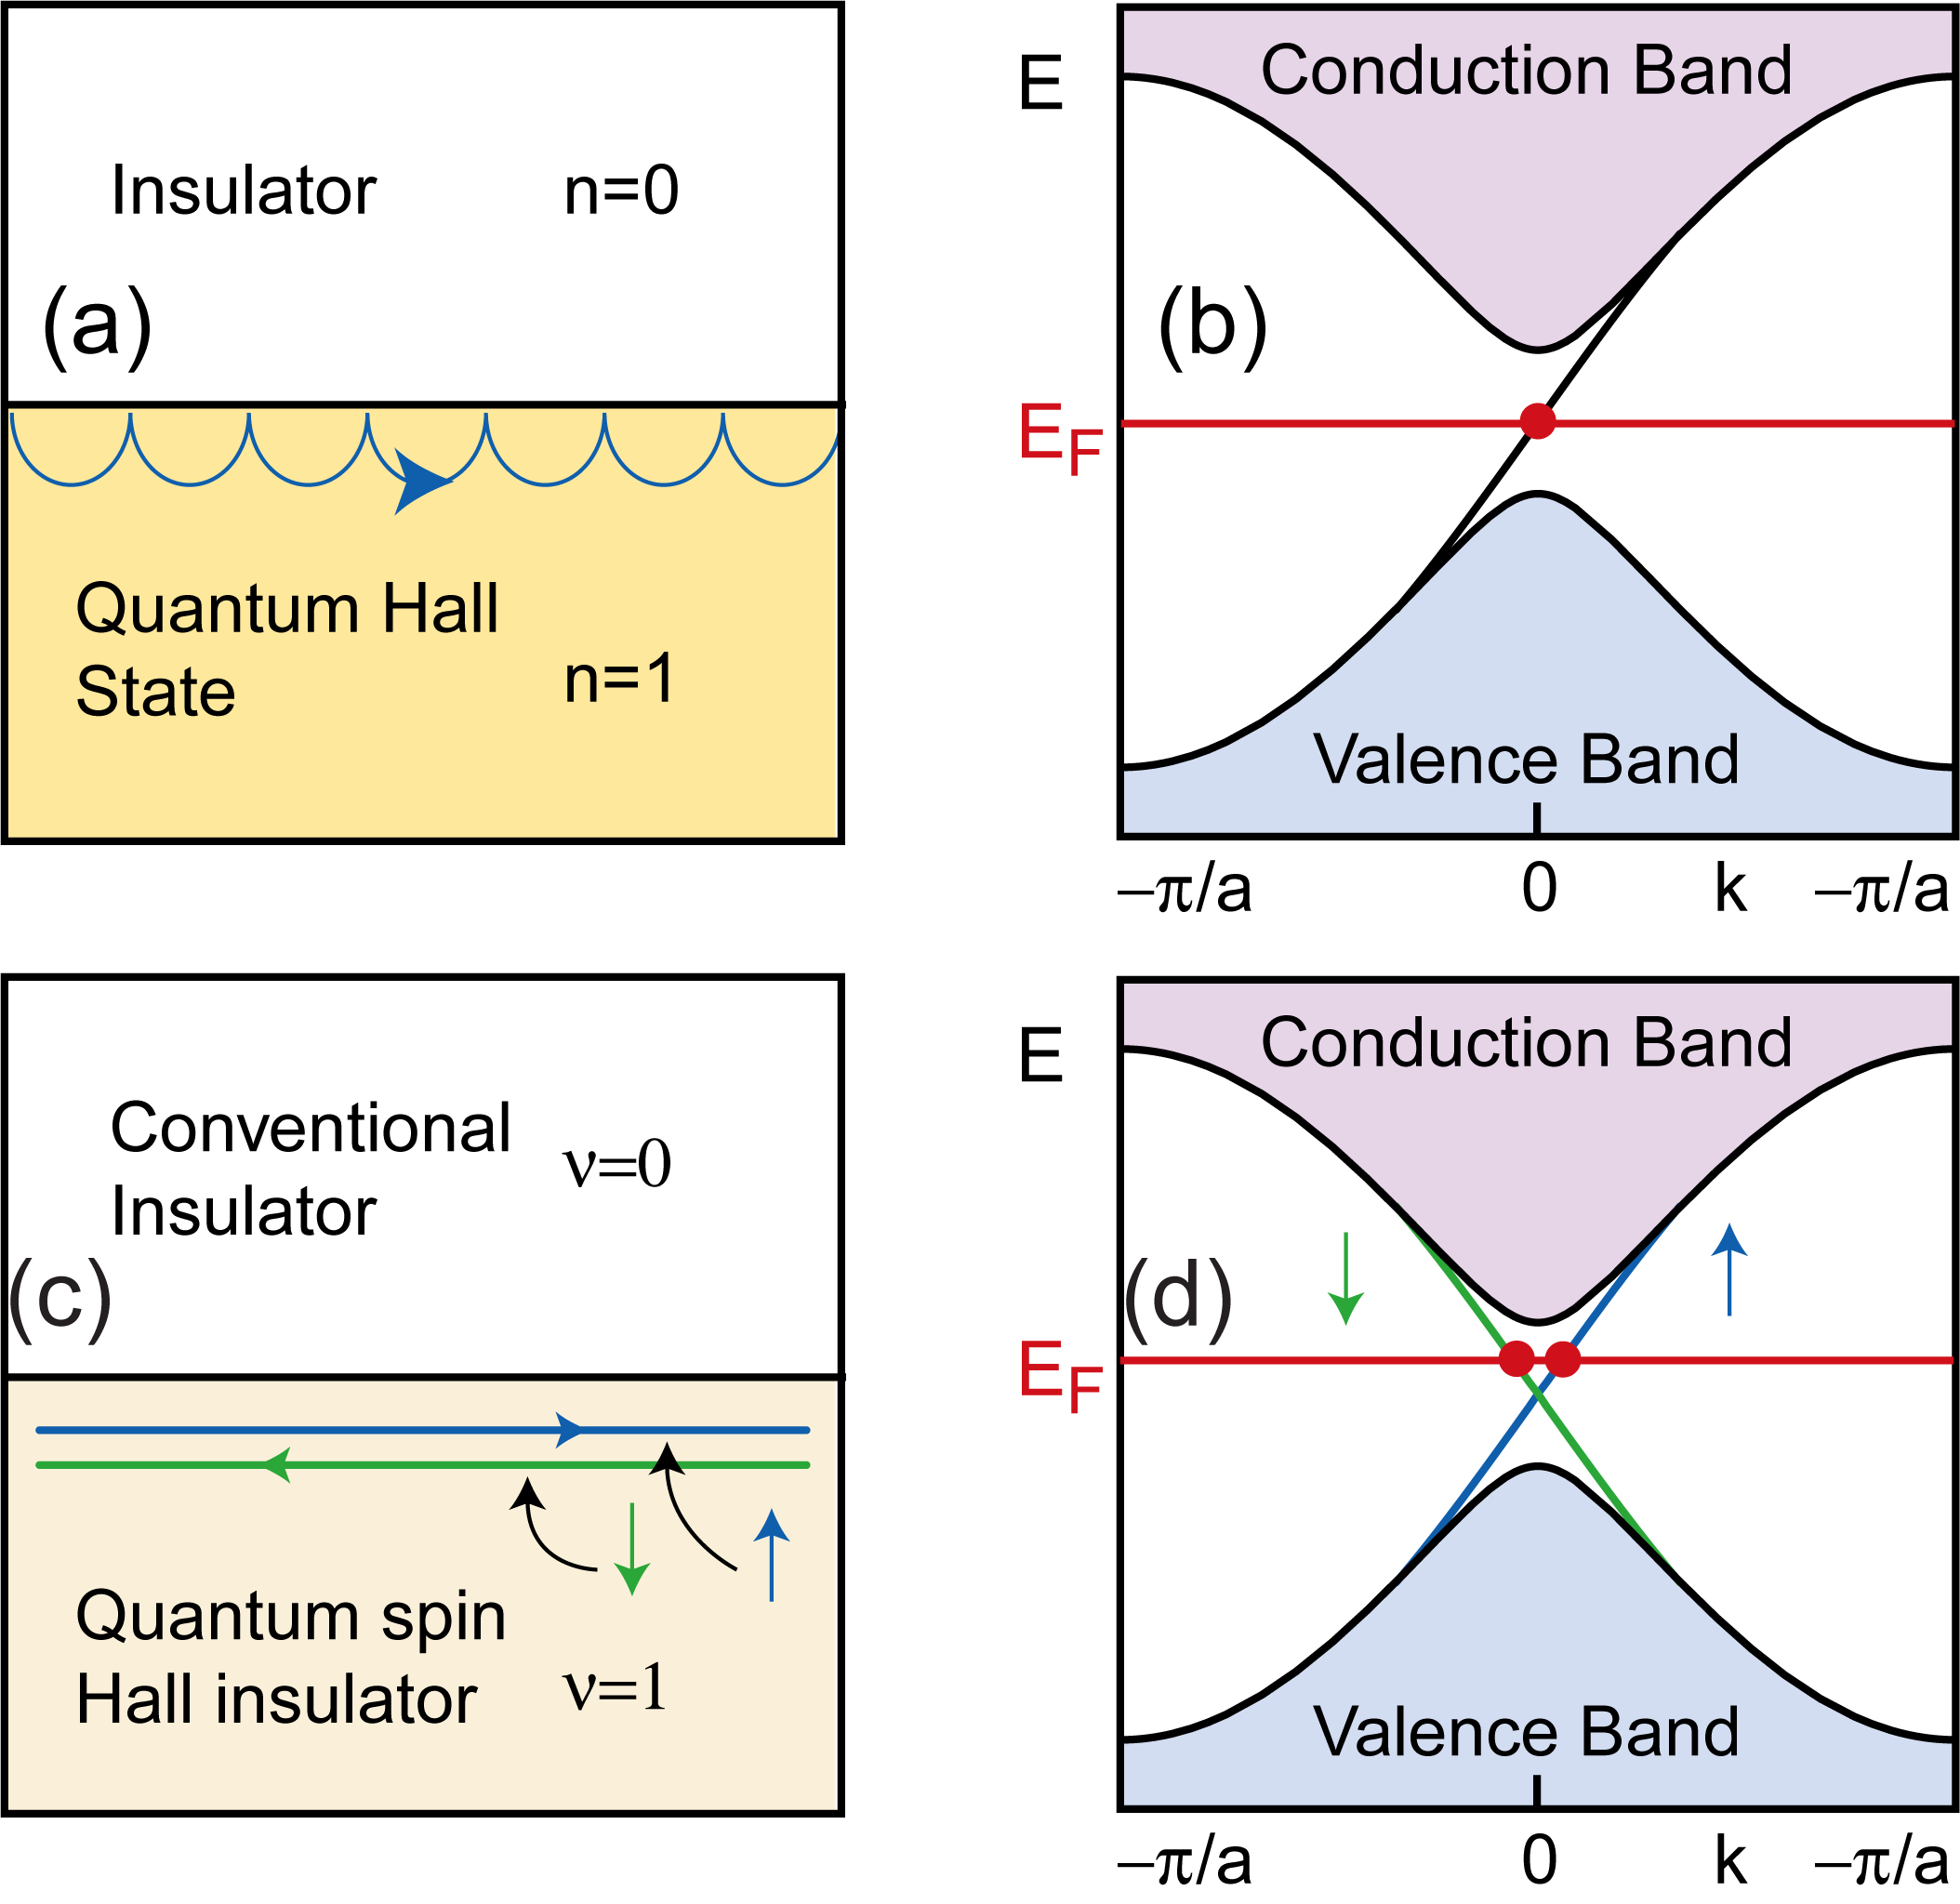
\includegraphics[scale=0.5]{pic/fig1.png}
\caption{(a)整数量子霍尔效应示意图。(b)整数量子霍尔效应能带示意图。(c)整数量子自旋霍尔效应示意图。(d)整数量子自旋霍尔效应能带示意图\cite{re60}。}\label{fig1}
\end{figure}
由加磁场产生的整数量子霍尔效应(QHE)以及由晶体自发磁化产生的反常量子霍尔效应(QAHE)都是破坏时间反演对称(TRS)的,但还存在一种满足TRS的量子自旋霍尔效应(QSHE),1988年F.Duncan M.Haldane在六角点阵中通过引入一个净磁通为零的位相,首次在理论上提出了一个不需要宏观磁场就可以实现QSHE,并计算拓扑保护的表面态\cite{re3}。这种新的量子态可以在存在自旋轨道耦合(SOC)的系统中出现,由于系统满足TRS,所以(\ref{chern_num})中的积分在整个布里渊区(BZ)中为零,也就是陈数为零,这个时候就需要一个新的拓扑不变量来描述QSHE。

\begin{figure}[h]
	\centering
	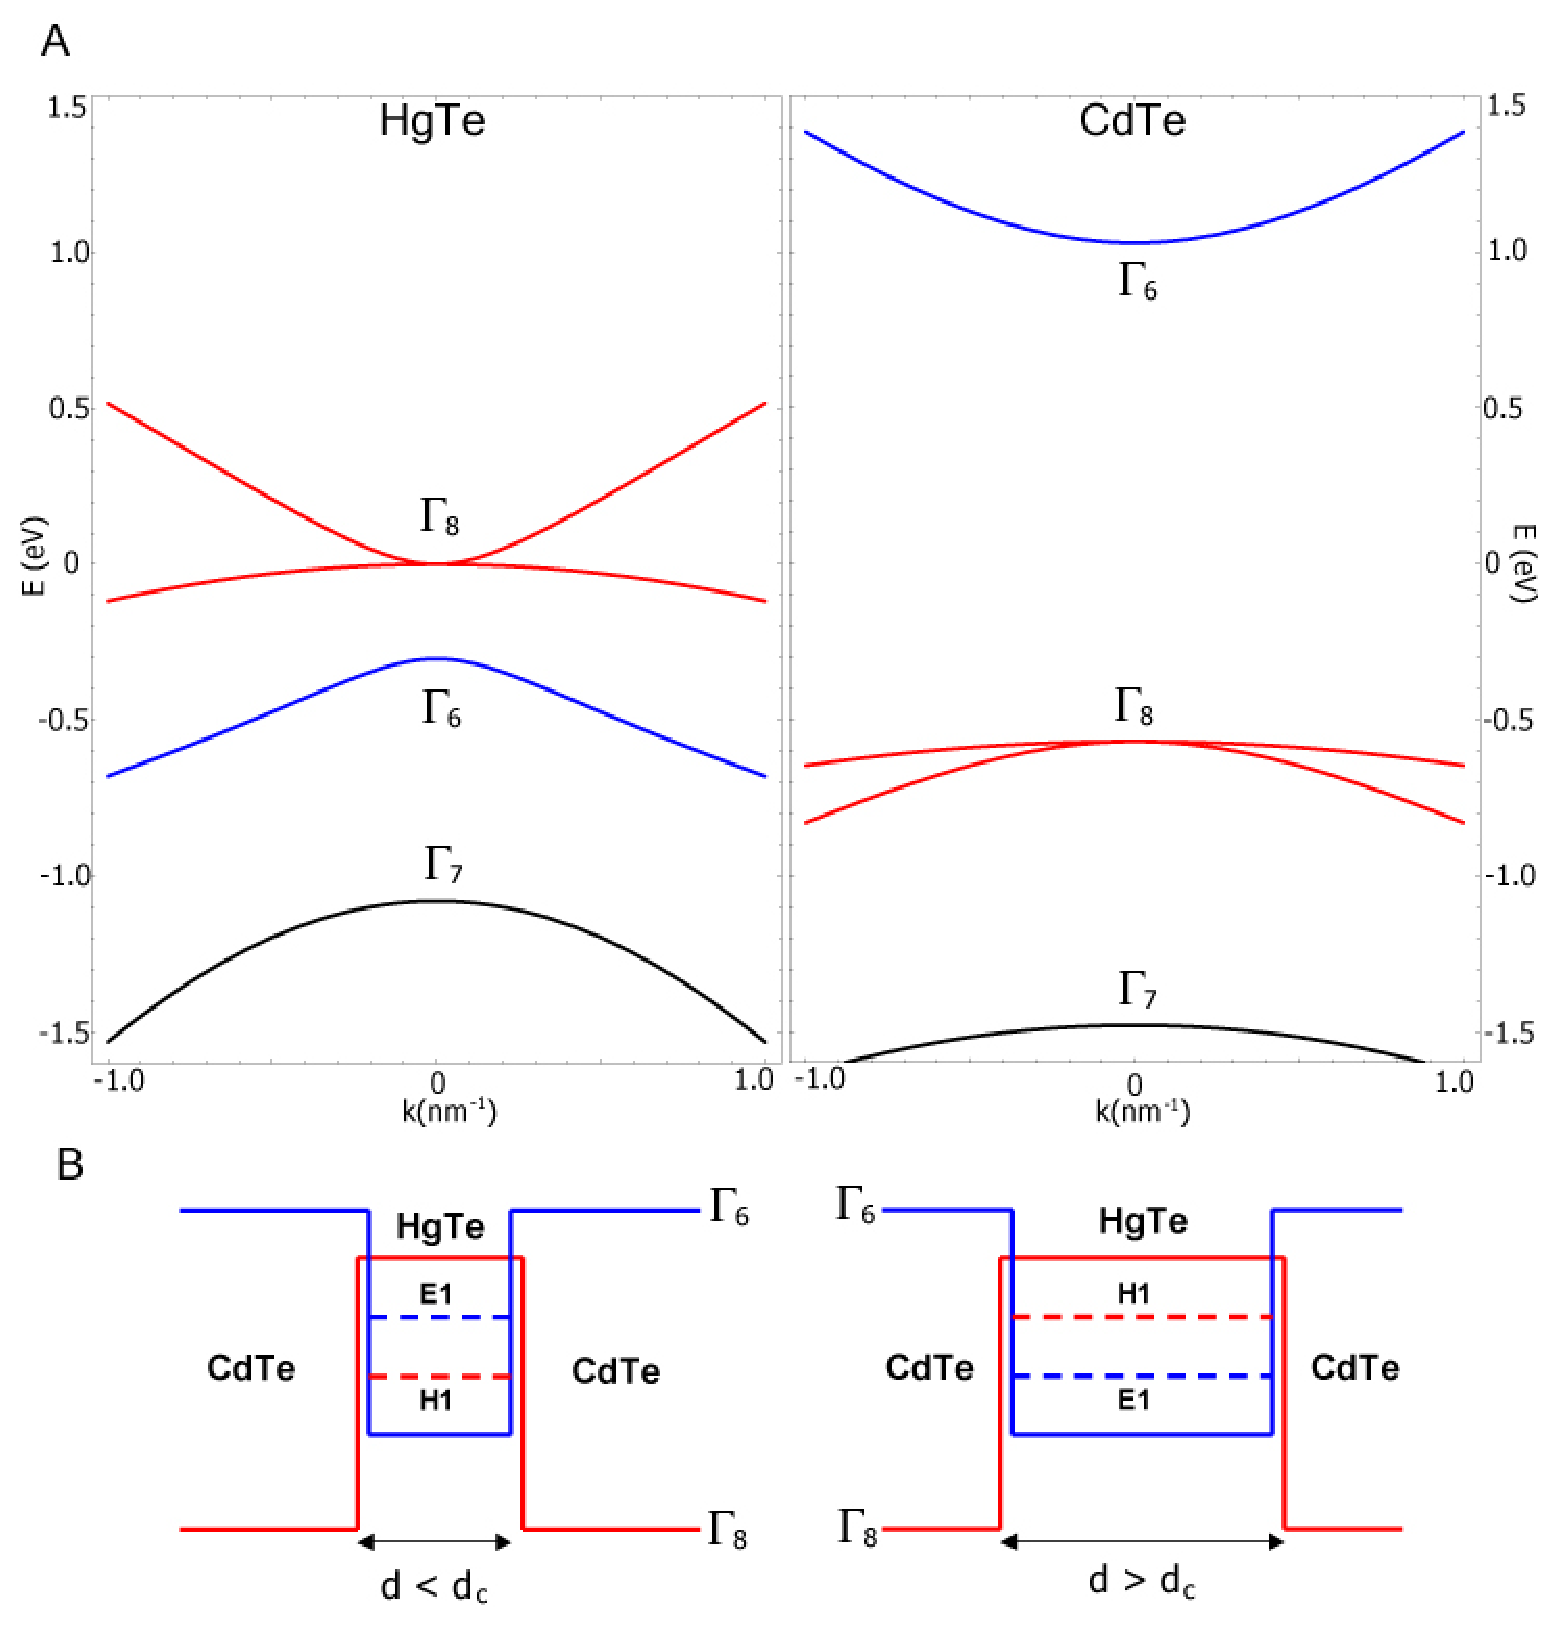
\includegraphics[scale=0.35]{pic/fig2.eps}
	\caption{A,HgTe与CdTe在布里渊区$\Gamma$点附近的体能带结构。B,CdTe/HgTe量子阱结构中正常态$d<d_c$与$d>d_c$的能级结构示意图\cite{re4}。}\label{fig2}
\end{figure}

 当一个系统哈密顿量满足TRS的时候,由Krammer定理可以知道此时每一个本征态的简并度为2,Krammer对在BZ中一定存在简并对。对于无自旋的粒子,时间反演算符为$\mathcal{T}=\mathcal{K}$,这里$\mathcal{K}$是复共轭算符 此时$\mathcal{T}^2=1$;对于有自旋的粒子,时间反演算符为$\mathcal{T}=e^{i\pi S_y}\mathcal{K}$,此时满足$\mathcal{T}^2=-1$。如图\ref{fig1}(d)所示,由于QSHE是时间反演不变的,所以它的连接价带和导带的表面态是由两支自旋动量都相反的表面态组成,而这两支表面态的交点正是时间反演不变动量点。这种表面态在实空间中的表现则如图\ref{fig1}(c)所示,系统与环境的交界面处存在着两个导电通道,其中输运方向和自旋方向都是相反的,是由时间反演对称保护的,所以电子的背散射是被禁止导致电子的无耗散运动,形成了电子输运的高速公路,正是这种特殊的性质,为将来量子器件的应用开启了新的大门。

\begin{figure}[h]
\centering
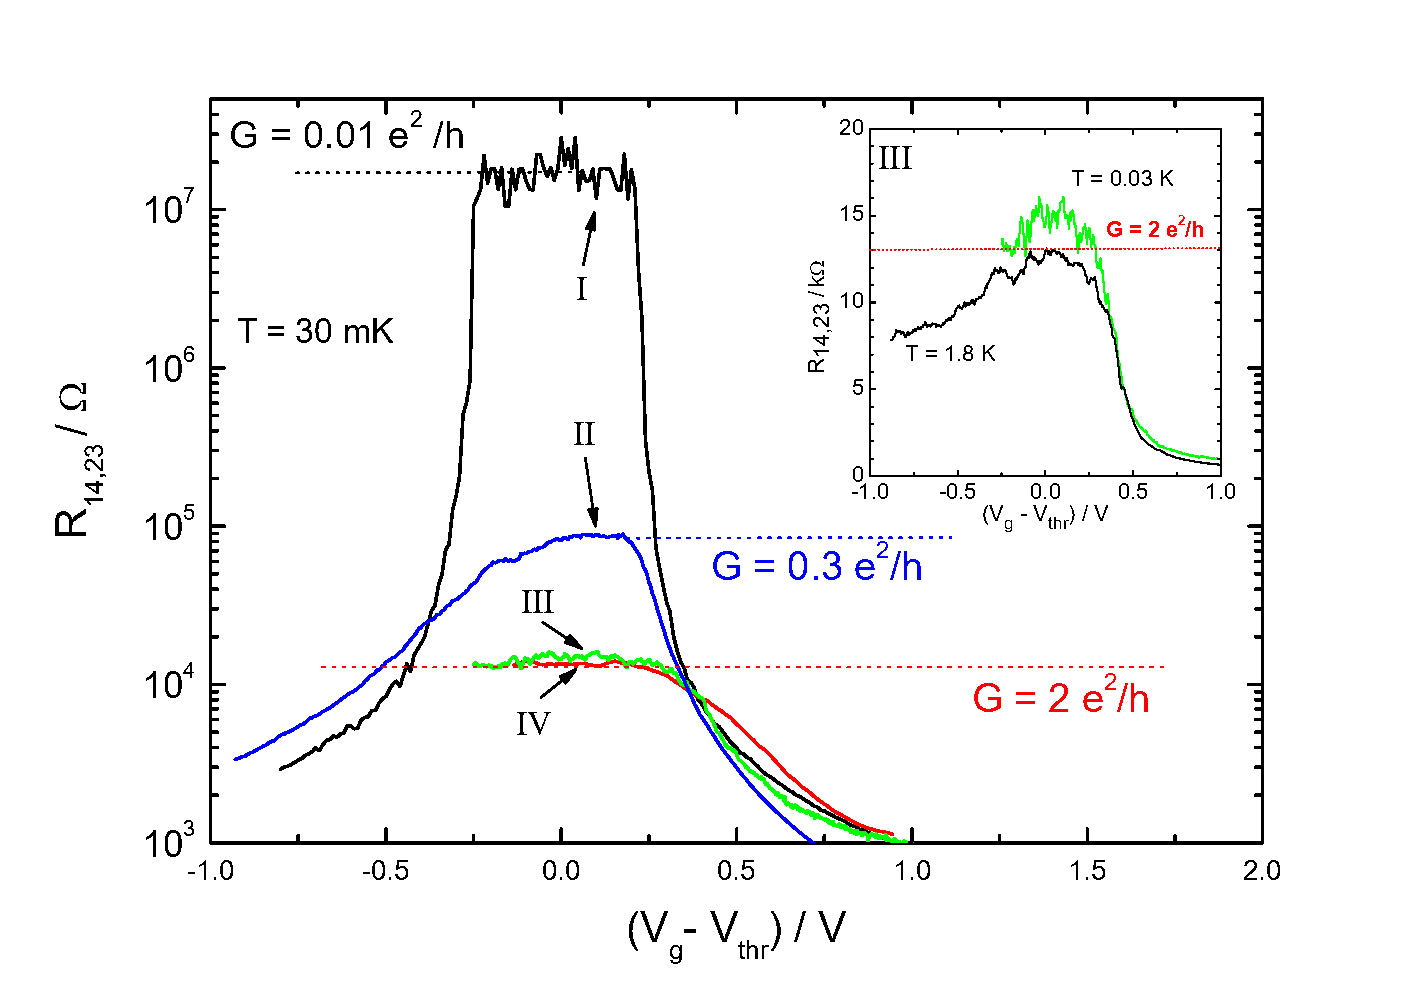
\includegraphics[scale=0.3]{pic/fig3.png}
\caption{HgTe/CdTe量子阱霍尔电阻随HgTe厚度的变化\cite{re5}。}\label{fig3}
\end{figure}

 实现拓扑绝缘体需要较强的SOC来将体态能带打开一个小的能隙,因为SOC起源于相对论效应,而元素周期表中越重的元素其相对论效应越强,则在真实材料体系中实现QSHE需要在较重的元素中搜寻。2006年张首晟等人通过理论语言在HgTe/CdTe的量子阱组成的三明治结构中,通过调节量子阱的厚度可以实现能带反转,进而实现QSHE如图\ref{fig2}\cite{re4}。实验上很快就在CdTe/HgTe/CdTe的量子阱中通过调节HgTE的厚度,发现霍尔电导的稳定平台,且不受样品厚度等其它因素的影响如图\ref{fig3}\cite{re5}。这是实验上首次确认了量子自旋霍尔效应。
%======================================================
\subsection{拓扑超导体}
  1911年,H.K.Onnes在研究金属汞处于极低温下的物性时,发现汞的电阻在温度降低的时候也慢慢变小,但是在温度达到4.2K时电阻突然变为0\cite{re7},这种有着零电阻的新物态被Onnes称为超导态,并将电阻突然变为0时的温度称为超导体的转变温度(T$_c$),之后在1933年W.Meissner等人发现了除零电阻外超导体的第二种特性;完全抗磁性,即Meissner效应\cite{re8}。零电阻和完全抗磁性是判断超导体的两个基本的判断证据。在超导现象被发现之后,科学家致力于寻找正确的微观机制来解释这一机制,直到1957 J. Bardeen,L. N. Cooper, J. R. Schrieffer三人共同提出了BCS理论\cite{re9},从理论上成功的解释了超导现象。之后科学家发现了另外一种转变温度远大于BCS理论所预言极限的超导材料YBa$_2$Cu$_3$O$_y$(YBCO),将超导的转变温度推到了液氮沸点以上,研究人员在不断的提高超导体的转变温度的同时,也在理论上探索着这种高温超导体的形成机理\cite{re10}。随着拓扑绝缘体在理论语言及实验验证的进展\cite{re4,re5},因为绝缘体与描述超导体的Bogoliubov–de Gennes(BdG)哈密顿量之间的相似性,准粒子的BdG哈密顿量即对应着能带绝缘体的哈密顿量,超导体的能隙即对应着能带绝缘体的能隙, 研究人员开始关注超导体的拓扑性质\cite{re11}。

 最简单的理解时间反演不变拓扑超导体的方式是和拓扑绝缘体进行类比,二维(2D)手性拓扑超导体是类似于量子霍尔效应的超导体,一个陈数为$N$的量子霍尔态有$N$个手性边界态,对于手性的拓扑超导体如果其拓扑量子数为$\mathcal{N}$则有$\mathcal{N}$个手性的马约拉纳边界态。因为BdG哈密顿量的正能态与负能态描述的是相同的物理自由度,所以每个马约拉纳手性边界态只有量子霍尔效应种的手性边界态一半的自由度,所以手性边界态是2D最小化的拓扑边界态。手性拓扑超导体与量子霍尔态的相似性如图\ref{fig4}上半部分所示。
\begin{figure}[h]
	\centering
	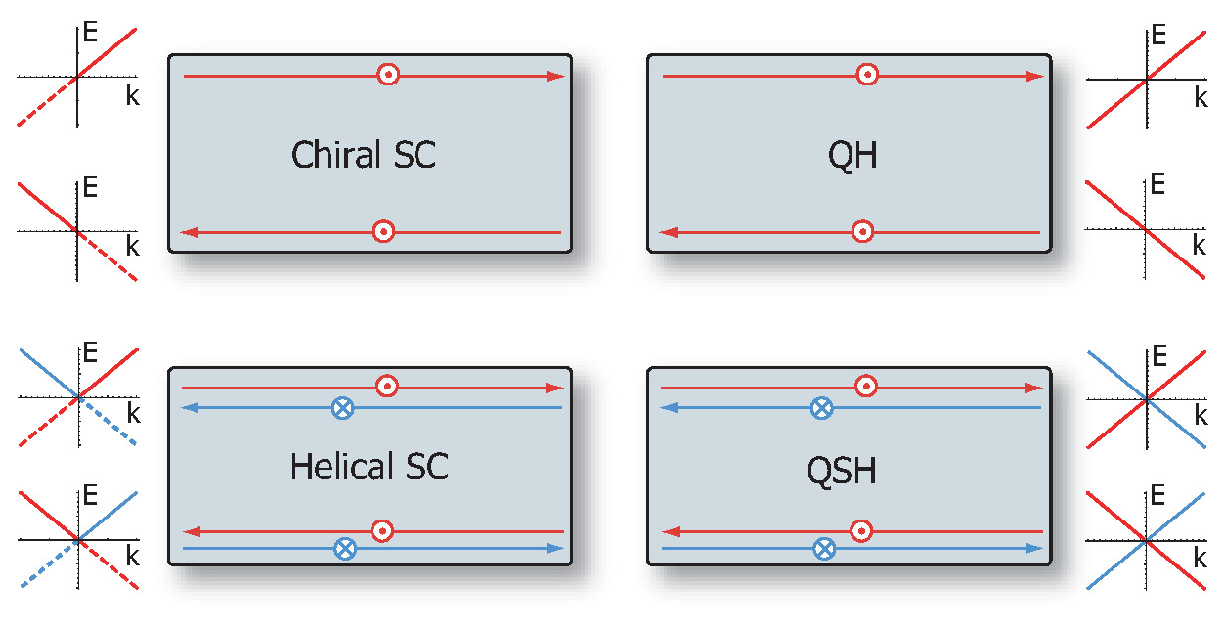
\includegraphics[scale=0.5]{pic/fig4.eps}
	\caption{(a)2D手性超导体与量子霍尔态的比较。(b)2D TRS拓扑超导体与量子自旋霍尔绝缘体比较\cite{re6} 。}\label{fig4}
\end{figure}
依照相同的逻辑,同样可以考虑和量子自旋霍尔效应类似的超导态,一个螺旋拓扑超导体,自旋向上的费米子组成$p_x+ip_y$的态,自旋向下的费米子组成$p_x-ip_y$的态。这样态存在一个边界上存在绕行方向相反的螺旋马约拉纳边界态且体态不存在能隙关闭点。相反,时间反演不变拓扑绝缘体的边界态是有两倍自由度的螺旋态Dirac费米子。对于量子自旋霍尔效应态,边界态的不能存在质量项,这是由时间反演对称保护的。因此,这样的超导相是由时间反演对称保护的,可以由$\mathit{Z}_2$拓扑不变量描述\cite{re12}。

 超导电子配对为$p_x\pm ip_y$的超导体本身就具有拓扑性质,但是$p$波电子配对在自然界是非常稀少的,研究人员开始提出其他方案来实现拓扑超导。2008年Fu和Kane两人提出了利用三维(3D)拓扑绝缘体的表面态近邻一个超导体,可以在外加磁场产生的Vortex中心束缚马约拉纳零能模\cite{re19},如图\ref{fig5}(a)所示,在3D拓扑绝缘体表面放置两块分开的$s$-波超导体,对应的项为分别是$\phi$和0,如果改变其中一块超导体的位相$\phi$,则体系的能带也会随之发生改变,当$\phi=\pi$时正好对应着体态能隙关闭点,即图\ref{fig5}(b)所示。对于这样的一个异质结结构,此时系统的边界处会存在马约拉纳零能模。同样的也可以构造一个图\ref{fig5}(c)所示的三角异质结,这样通过调节相互之间的超导位相,可以实现马约拉纳零能模的控制,这种对马约拉纳零能模的操作也为拓扑量子计算提供了一定的基础条件。图\ref{fig5}(d)中灰色区域所示的即为马约拉纳零能模可以存在的区域。
\begin{figure}[h]
\centering
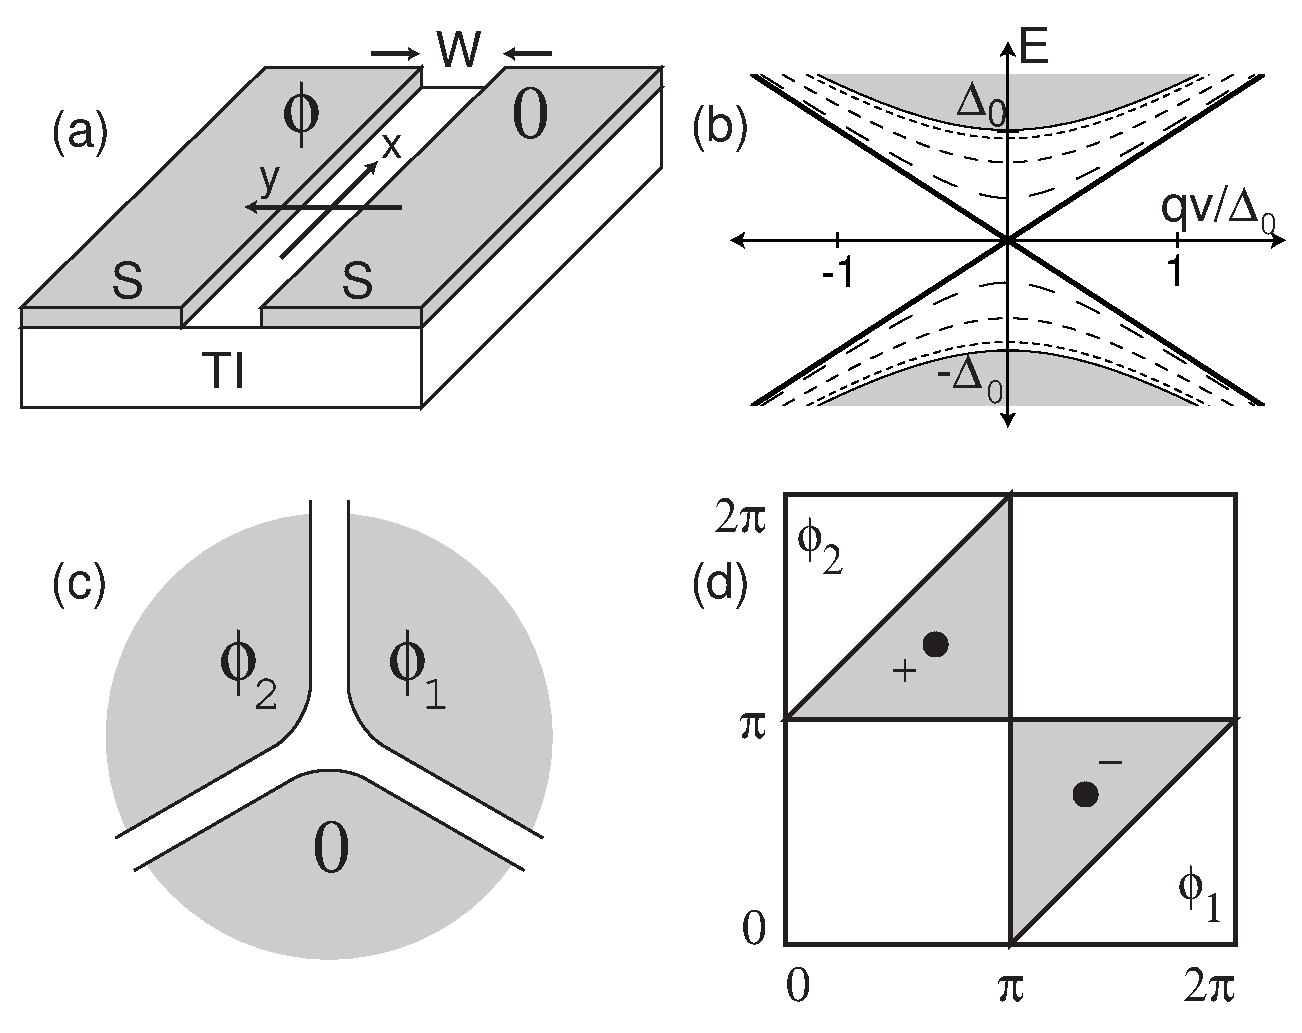
\includegraphics[scale=0.5]{pic/fig5}
\caption{(a)STIS异质结;(b)STIS线性结的能带图;(c)超导三相结;(d)三线结相图\cite{re19}。}\label{fig5}
\end{figure}

研究人员同样发现在存在Rashba SOC的2D电子气中
\begin{equation}
H=\int d^2x\psi^\dagger\left[\mathbf{p}^2/2m+\alpha(\mathbf{\sigma}\mathbf{\times p})\cdot\hat{\mathbf{z}}-\mu\right]
\end{equation}
也可以利用近邻效应在电子气中诱导$s$-波配对,此时系统每个分立的费米面都会形成非平庸的超导体,但是两个费米面上的马约拉纳费米子会相互湮灭,所以在Rashba系统中诱导$s$-波超导配对是平庸的。之后研究人员发现通过在哈密顿量中引入破坏时间反对称的$M\sigma_z$项可以得到非平庸的超导相,它会把$\mathbf{k}=0$处的简并分离开来。如果将化学势被调节到$|\mu|<|M|$则半径较小的费米面会消失,所以仅剩下外部半径较大的费米面上诱导$s$-波超导配对,从而体系变成拓扑非平庸相\cite{re20,re21,re22}。

 和拓扑绝缘体相同,拓扑超导体在处于拓扑相时也存在非平庸的边界态,和拓扑绝缘体不同的是在这里可以存在局域的马约拉纳费米子\cite{re12,re13,re14,re15,re16}。马约拉纳费米子的反粒子是它本身($\gamma^\dagger=\gamma$),虽然并没有被却认为基本粒子,但是在凝聚态体系的准粒子激发中可以产生这种粒子。相比较于其它的基本粒子,马约拉纳费米子满足非阿贝尔统计,属于非阿贝尔费米子,而且它与激发态之间的能隙对应的正是超导能隙,具有较好的抵抗环境噪声的能力,可以稳定存在,同时也具有高度非局域化性质,这两种性质在实现拓扑量子计算方面有很大的应用价值\cite{re17,re18}。
%======================================================
\subsection{高阶绝缘体}
 最近研究人员发现了一种新的拓扑相,被称为高阶拓扑\cite{re23,re24,re25,re26,re27,re28,re29,re30,re31,re32,re33,re34,re35,re36,re37,re38,re39,re40}。对于通常的拓扑物态来说,其非平庸的边界态总是出现在比系统维度低一维的维度中,比如二维拓扑绝缘体的边界态是一维(1D)的。但是这种新的拓扑相其边界态可以出现的维度比系统维度可以低两维或者三维,即一个$d$维的高阶拓扑态,它拓扑保护的无能隙边界态会出现在$d-n$维$(n\le d)$。比如一个2D$(d=2)$的高阶拓扑物态其边界态会出现的系统的角落($d=2,n=2$),3D$(d=3)$的高阶拓扑态其边界态则会出现在系统的棱$(n=2)$或者角落$(n=3)$,如图\ref{fig6}所示。
\begin{figure}[h]
\centering
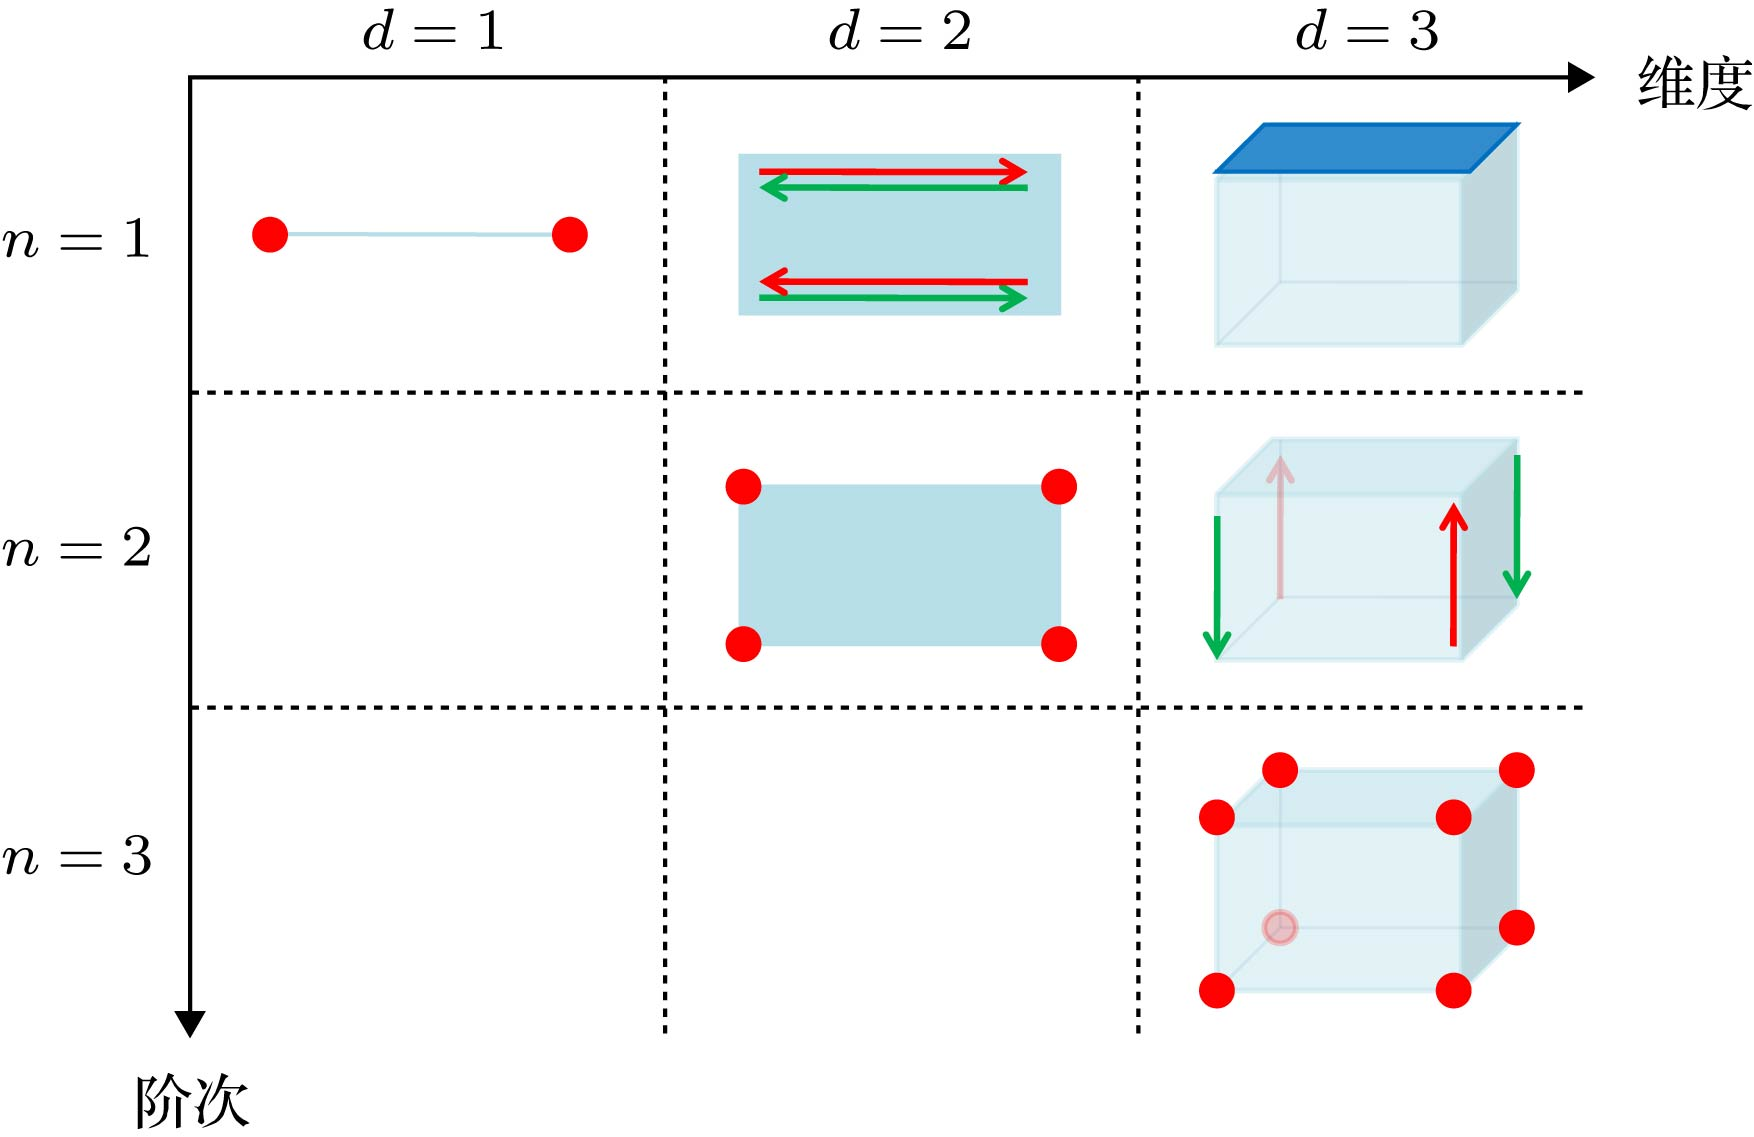
\includegraphics[scale=1.7]{pic/fig6}
\caption{拓扑物态的边界态示意图;$n=1$的行对应传统的拓扑物态, 其具有比系统维度低一维的无能隙边界态; $n\geq 2$的行对应高阶拓扑物态, 其具有比维度低n维的无能隙边界态\cite{re40}。}\label{fig6}
\end{figure}

 一个描述高阶拓扑绝缘体的四带Bloch哈密顿量为
\begin{equation}
H_c(\mathbf{k})=(M+t\sum_i\cos k_i)\tau_z\sigma_0+\Delta_1\sum_i\sin k_i\tau_x\sigma_i+\Delta_2(\cos k_x-\cos k_y)\tau_y\sigma_0\label{hoti}
\end{equation}
这里泡里矩阵$\sigma_i,\tau_i$(i=x,y,z)分别代表着自旋自由度和轨道自由度。当$1<|M|<3$且$\Delta_2=0$的时候(\ref{hoti})描述的是一阶3D拓扑绝缘体。此时哈密顿量满足时间反演对称$\mathcal{T}H_c(\mathbf{l})\mathcal{T}^{-1}=H_c(\mathbf{k})$,$\mathcal{T}=\tau_0\sigma_y\mathcal{K}$,这里$\mathcal{K}$代表复数共轭操作。当$\Delta_2=0$哈密顿量(\ref{hoti})具有$\hat{C}_4^z$旋转对称$\hat{C}_4^zH_c(\mathbf{k})(\hat{C}_4^z)^{-1}=H_c(D_{\hat{C}_4^z}\mathbf{k})$,这里旋转操作$\hat{C}_4^z\equiv \tau_0e^{-i\frac{\pi}{4}\sigma_z}$和$D_{\hat{C}_4^z}\mathbf{k}=(-k_y,k_x,k_z)$。

 正比于$\Delta_2$的这一项同时破坏了$\mathcal{T}$和$\hat{C}_4^z$对称性,但是对于它们的组合操作$\hat{C}_4^z\mathcal{T}$是反对易的
\begin{equation}
(\hat{C}_4^z\mathcal{T})H_c(\mathbf{k})(\hat{C}_4^z\mathcal{T})^{-1}=H_c(D_{\hat{C}_4^z\mathcal{T}}\mathbf{k}),\quad D_{\hat{C}_4^z\mathcal{T}}\mathbf{k}=(k_y,-k_x,-k_z)
\end{equation}
由于$\left[\hat{C}_4^z,\mathcal{T}\right]=0$,组合操作$\hat{C}_4^z\mathcal{T}$满足$(\hat{C}_4^z\mathcal{T})^4=-1$。
\begin{figure}[h]
\centering
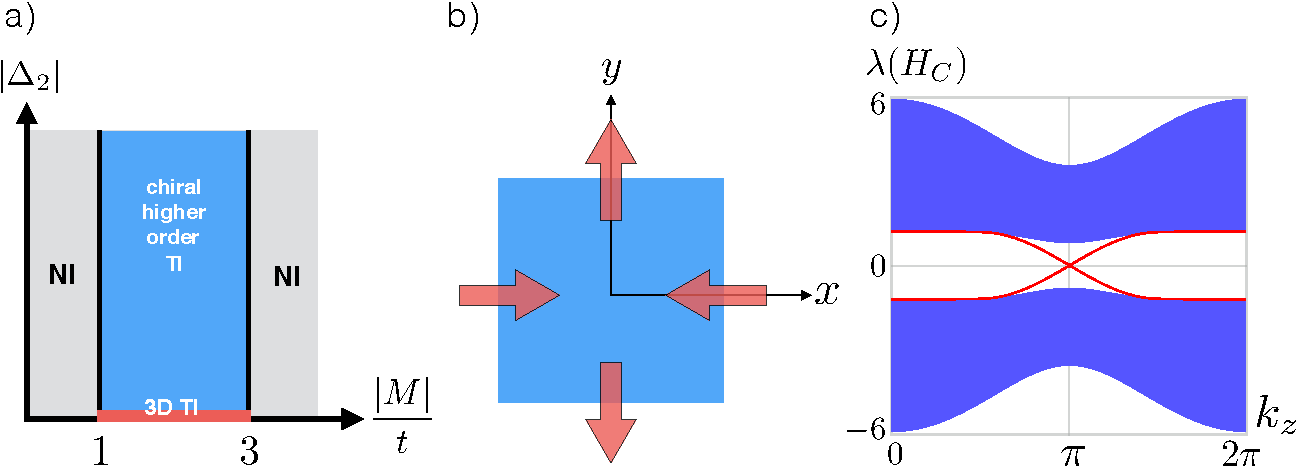
\includegraphics[scale=0.7]{pic/fig7}
\caption{手性高阶拓扑绝缘体;(a)哈密顿量(\ref{hoti})的相图,(b)一个元胞内满足$\hat{C}_4^z\mathcal{T}$的非共线反铁磁,(c)存在手性棱态(红色)的哈密顿量(\ref{hoti})的能谱图\cite{re23}。}\label{fig7}
\end{figure}
哈密顿量(\ref{hoti})的相图如图(\ref{fig7})(a)所示,当$1<|M/t|<3$且$\Delta_1,\Delta_2\neq 0$时,系统处于3D手性高阶拓扑绝缘体相。$x$和$y$方向取开边界条件,$z$方向取周期边界时,体系的能谱如图\ref{fig7}(c)所示,红色代表的手性棱模穿过了体态的能隙。从物理上讲,$\Delta_2$对应的项破坏了时间反演,对应着在$x$和$y$方向上相反的轨道流。当$\Delta_2$无限小的时候,它的主要作用是会在3D拓扑绝缘体的(100)与(010)表面上打开一个质量相反的能隙,这时候四个棱就是就会变成Dirac质量变号的质量畴壁,从而在棱上形成无能隙的手性模,也正好就是高阶拓扑绝缘体中的棱模。另外一种打破时间反演并保持$\hat{C}_4^z\mathcal{T}$的物理机制是在元胞内存在$(\pi,\pi,0)$方向上的非共线反铁磁序,如图\ref{fig7}(b)所示。这里值得注意的是,即使$\Delta_2$是有限大小的值,3D拓扑绝缘体的(001)面始终是无能隙的,由于这个表面上的Dirac锥是受$\hat{C}_4^z\mathcal{T}$保护的,表面在这个操作下是不变的,且存在一个Kramers类似的简并。通过第一性原理计算,研究人员同样确定SnTe在一定方向上施加压力是一种可以实现手性高阶拓扑绝缘体的材料\cite{re23}。
%======================================================
\subsection{高阶拓扑超导体}
 随着实验上在100K温度下实现了2D拓扑绝缘体\cite{re41,re42},研究人员提出利用超导体的近邻效应,将2D拓扑绝缘体放置在一个高温超导体的基底上从而在拓扑绝缘体中诱导出$d$-波配对,从而来实现2D的高阶拓扑超导体\cite{re28,re27}。与传统的一阶拓扑超导体不同的是,此时系统中马约拉纳零能态出现在样品的角落处的,如图\ref{fig8}所示。
\begin{figure}[h]
\centering
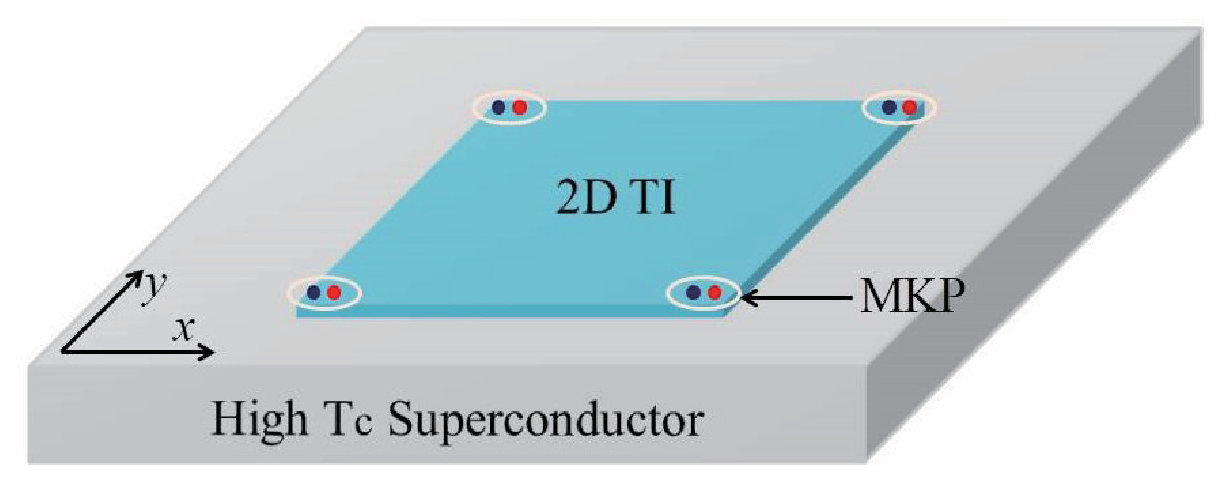
\includegraphics[scale=0.7]{pic/fig8}
\caption{示意图展示;一个2D拓扑绝缘体长在$d$-波或者$s_\pm$-波的高温超导体上,零能马约拉纳Kramers对(MKP)将会出现在2D拓扑绝缘体的角落\cite{re28}。}\label{fig8}
\end{figure}
产生这个结果的物理图像如下:2D拓扑绝缘体的边界态是由1D无质量的Dirac费米子描述的,当通过近邻效应将2D拓扑绝缘体放置在超导体上面时,由于超导体的近邻效应,会在拓扑绝缘体表面上诱导出电子配对,这种形式的电子配对会将拓扑绝缘体无能隙的边界态打开一个能隙,从而引入一个Dirac质量项。由于超导配对的对称性(比如说$d$-波配对),如图\ref{fig22}所示,所以在相邻的两个方向上电子配对是相反的,导致相邻边界态上诱导出的质量是相反的,从而在相邻两条边界的相交角落处,形成类似质量畴壁,由于体系存在粒子空穴对称,这个束缚态即对应着零能的马约拉纳角态。
\begin{figure}[h]
	\centering
	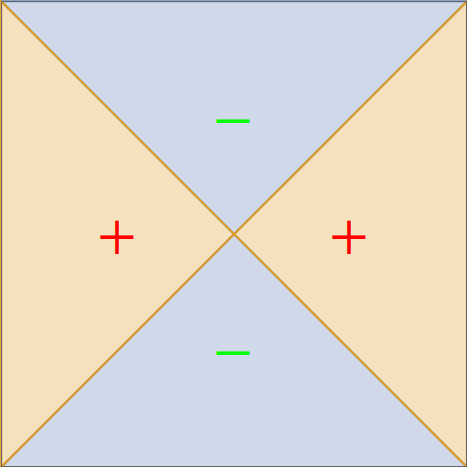
\includegraphics[scale=0.5]{pic/dwave}
	\caption{动量空间中$d$波超导体电子配对符号}\label{fig22}
\end{figure}
 根据上面的解释,这个结果的主要来源就是边界态,那么从一个2D拓扑绝缘体模型出发,之后通过近邻效应在2D拓扑绝缘体上诱导出超导配对来进行研究。研究人员将超导电子配对作为2D拓扑绝缘体的本征属性直接加入到了拓扑绝缘体的哈密顿量中,BdG哈密顿量写为
\begin{equation}
\begin{aligned}
\hat{H}&=\sum_\mathbf{k}\Psi_\mathbf{k}^\dagger H(\mathbf{k})\Psi_\mathbf{k}\\
\Psi^\dagger_\mathbf{k}&=(c^\dagger_{a\uparrow\mathbf{k}},c^\dagger_{b\uparrow\mathbf{k}},c^\dagger_{a\downarrow\mathbf{k}},c^\dagger_{b\downarrow\mathbf{k}},c_{a\downarrow\mathbf{-k}},c_{b\downarrow\mathbf{-k}},c_{a\uparrow\mathbf{-k}},c_{b\uparrow\mathbf{-k}})
\end{aligned}
\end{equation}
\begin{equation}
\begin{aligned}
H(\mathbf{k})&=M(\mathbf{k})\sigma_z\tau_z+A_x\sin k_x\sigma_xs_z+A_y\sin k_y\sigma_y\tau_z+\Delta(\mathbf{k})s_y\tau_y-\mu\tau_z\\\label{hoti2}
\end{aligned}
\end{equation}
这里泡里矩阵$s_i,\sigma_i,\tau_i$分别在自旋空间($\uparrow,\downarrow$),轨道空间$(a,b)$,和粒子空穴空间。质量项$M(\mathbf{k})=m_0-t_x\cos k_x-t_y\cos k_y$,和$A_{x/y}$代表动能项代表着动能,$\Delta(\mathbf{k})$是超导配对,$\mu$是化学势。对于高温超导体,将配对取为
\begin{equation}
\Delta(\mathbf{k})=\Delta_0+\Delta_x\cos k_x+\Delta_y\cos k_y
\end{equation}
这个形式可以同时描述$d$-波和$s_\pm$-波这两种不同的配对形式。哈密顿量(\ref{hoti2})具有时间反演对称$\mathcal{T}H(\mathbf{k})\mathcal{T}^{-1}=H(-\mathbf{k})$,时间反演算符为$\mathcal{T}=is_y\mathcal{K}$,同时也满足粒子空穴对称$\mathcal{C}H(\mathbf{k})\mathcal{C}^{-1}=-H(-\mathbf{k})$,粒子空穴算符$\mathcal{C}=\tau_x\mathcal{K}$,$\mathcal{K}$代表复数共轭操作。

 接下来考虑铜基超导体中的$d$-波配对
\begin{equation}
\Delta_0=0,\qquad\Delta_x=-\Delta_y\equiv\Delta_d
\end{equation}
将哈密顿量$x$方向取开边界条件$y$方向取周期性边界条件(圆柱体结构),计算得到的能谱如图\ref{fig9}(a)所示,可以看到2D拓扑绝缘体的螺旋边界态在诱导出超导配对之后打开一个能隙,而从实空间的计算结果\ref{fig9}(b)也可以看到,系统的每个角落处都局域一个马约拉纳卡莱默对,其能量由于粒子空穴对称性的存在被限制在零能处。
\begin{figure}[h]
\centering
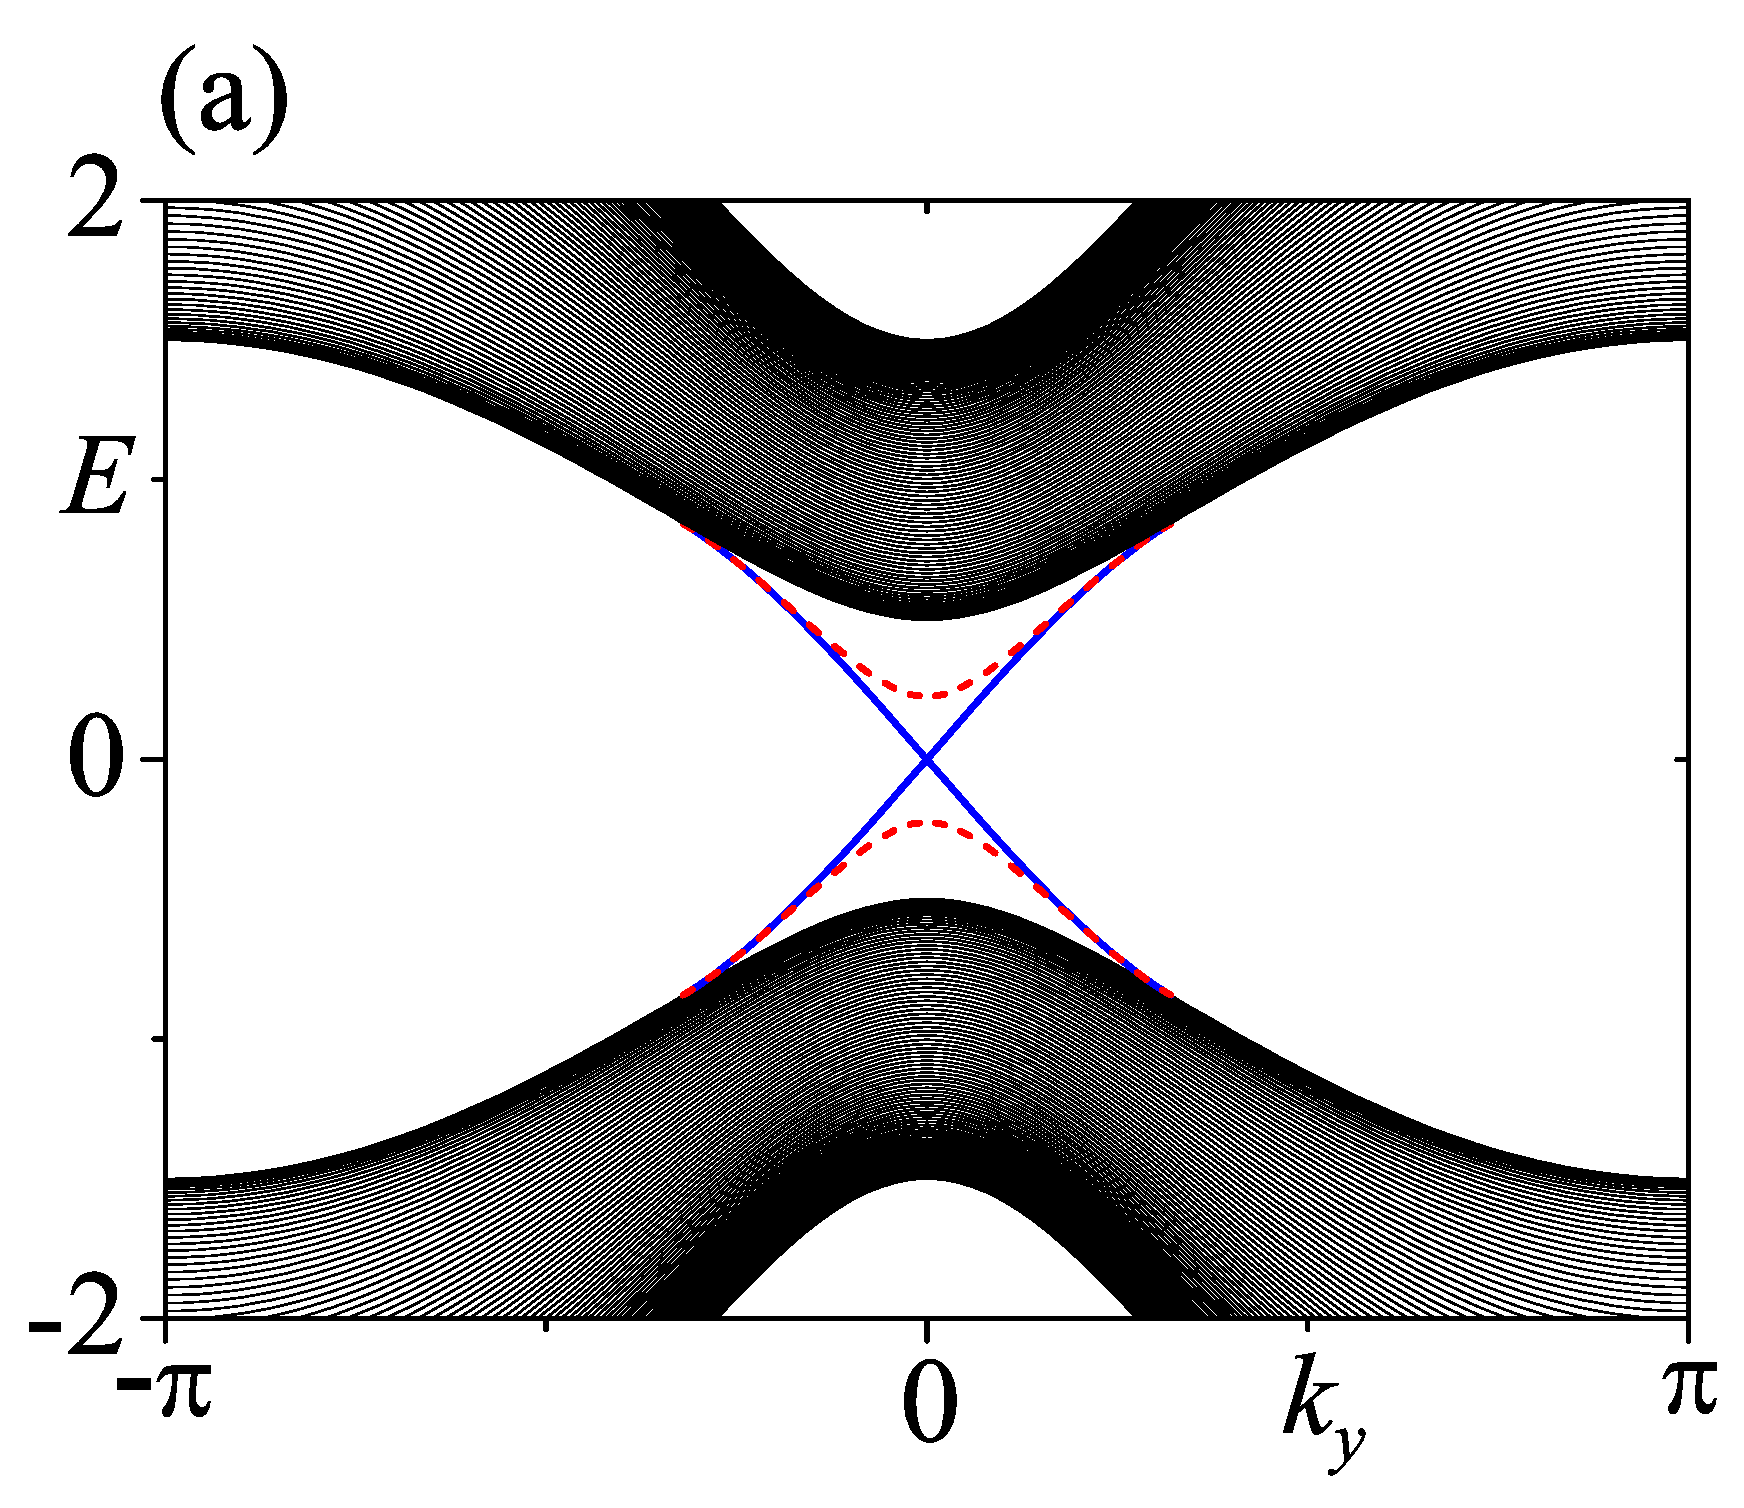
\includegraphics[scale=0.26]{pic/fig9}
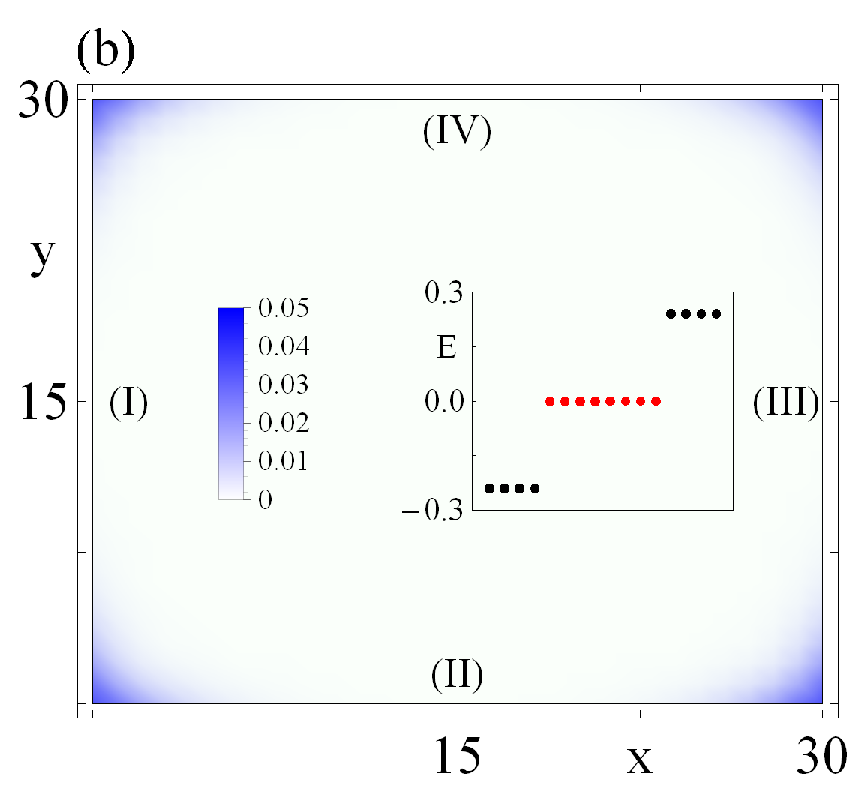
\includegraphics[scale=0.5]{pic/fig10}
\caption{(a)圆柱体结构能谱图;(b)四个MKP的波函数分布\cite{re28}。}\label{fig9}
\end{figure}
有趣的是,此时马约拉纳零能态并不是出现的vortex中心或者是原子链尾端,它出现在了2D系统的角落,这正是最近研究人员提出的高阶拓扑绝缘体以及高阶拓扑超导体的特征。这里晶体的对称性是被强调了的,但是现在这个体系出现角态并不依赖于晶体的对称性。这里需要提及的是,体态的$d$-波超导配对是有节点存在的($\Delta(\mathbf{k})=0$),马约拉纳卡莱默对将会与这些无能隙的模混合到一起,但是仍然可以利用STM进行观测,当隧穿电导在电压等于零的位置出现一个明显的电导峰的时候,即为有力的证据。

 接下来通过有效边界理论来得到一个更加直观的物理图像,首先将哈密顿量(\ref{hoti2})在$\Gamma=(0,0)$处做低能展开,并保留到二阶
\begin{equation}
H(\mathbf{k})=(m+\frac{t_x}{2}k_x^2+\frac{t_y}{2}k_y^2)\sigma_z\tau_z+\lambda_xk_x\sigma_xs_z+\lambda_yk_y\sigma_y\tau_z-\frac{1}{2}(\Delta_xk_x^2+\Delta_yk_y^2)s_y\tau_y\label{hoti2e}
\end{equation}
对于$d$-波超导体有$\Delta_x+\Delta_y=0$,对于2D拓扑绝缘体$m=m_0-t_x-t_y<0$保证在在没有超导配对的时候体系处于拓扑非平庸相。如图\ref{fig9}(b)所示,将正方形的四个边分别标记为(\uppercase\expandafter{\romannumeral1}),(\uppercase\expandafter{\romannumeral2}),(\uppercase\expandafter{\romannumeral3}),(\uppercase\expandafter{\romannumeral4}),这里先关注(\uppercase\expandafter{\romannumeral1})这条边,取$x$方向在实空间$k_x\rightarrow-i\partial_x$,将哈密顿量(\ref{hoti2e})分解成两部分$H=H_0+H_p$
\begin{equation}
\begin{aligned}
H_0(-i\partial_x,k_y)&=(m-t_x\partial_x^2/2)\sigma_z\tau_z-i\lambda_x\sigma_xs_z\partial_x\\
H_p(-i\partial_x,k_y)&=\lambda_yk_y\sigma_y\tau_z+\frac{\Delta_y}{2}s_y\tau_y\partial_x^2
\end{aligned}
\end{equation}
在这里忽略了$k_y^2$项,首先需要求解$H_0$的本征方程,然后将$H_p$当作微扰,所以$k_y^2$的贡献自然是可以忽略的。

 在边界条件$\psi_\alpha(0)=\psi_\alpha(+\infty)$下来求解$H_0\psi_\alpha(x)=E_\alpha\psi_\alpha(x)$可以得到四个零能解,其形式为
\begin{equation}
\psi_\alpha(x)=\mathcal{N}_x\sin(\kappa_1x)e^{-\kappa_2x}e^{ik_yy}\xi_\alpha
\end{equation}
归一化系数为 $|\mathcal{N}_x|^2=4|\kappa_2(\kappa_1^2+\kappa_2^2)/\kappa_1^2|$。(符号简记,$\kappa_1=\sqrt{|(2m_x/t_x)|-(\lambda_x^2/t_x^2)}$,$ \kappa_2=(\lambda_x/t_x)$)。旋量部分 $\xi_\alpha$ 满足 $\sigma_ys_z\tau_z=-\xi_\alpha$,可以将旋量部分选取为
\begin{equation}
\begin{aligned}
\xi_1&=|\sigma_y=-1\rangle\otimes|\uparrow\rangle\otimes|\tau_z=+1\rangle\\
\xi_2&=|\sigma_y=+1\rangle\otimes|\downarrow\rangle\otimes|\tau_z=+1\rangle\\
\xi_3&=|\sigma_y=+1\rangle\otimes|\uparrow\rangle\otimes|\tau_z=-1\rangle\\
\xi_4&=|\sigma_y=-1\rangle\otimes|\downarrow\rangle\otimes|\tau_z=-1\rangle
\end{aligned}
\end{equation}
在这个基矢的选取下,微扰部分$H_p$计算为
\begin{equation}
H_{\uppercase\expandafter{\romannumeral1},\alpha\beta}(k_y)=\int_{0}^{\infty}dx\psi^*_\alpha(x)H_p(-i\partial_x,k_y)\psi_\beta(x);
\end{equation}
最后得到有效哈密顿量为
\begin{equation}
H_{\uppercase\expandafter{\romannumeral1}}(k_y)=-A_yk_ys_z+M_{\uppercase\expandafter{\romannumeral1}}s_y\tau_y
\end{equation}
这里
\begin{equation}
M_{\uppercase\expandafter{\romannumeral1}}=\frac{\Delta_x}{2}\int_{0}^{\infty}dx\psi_\alpha^*(x)\partial_x^2\psi_\alpha(x)=\Delta_x\frac{m}{t_x}
\end{equation}
其它三个边界上的有效哈密顿量也可以通过相似方式求解得到,结果为
\begin{equation}
\begin{aligned}
H_{\uppercase\expandafter{\romannumeral1}}&=-A_yk_ys_z+M_{\uppercase\expandafter{\romannumeral1}}s_y\tau_y\\
H_{\uppercase\expandafter{\romannumeral2}}&=A_xk_xs_z+M_{\uppercase\expandafter{\romannumeral2}}s_y\tau_y\\
H_{\uppercase\expandafter{\romannumeral3}}&=A_yk_ys_z+M_{\uppercase\expandafter{\romannumeral3}}s_y\tau_y\\
H_{\uppercase\expandafter{\romannumeral4}}&=-A_xk_xs_z+M_{\uppercase\expandafter{\romannumeral4}}s_y\tau_y\\\label{edge1}
\end{aligned}
\end{equation}
每条边界上的质量项满足$M_{\uppercase\expandafter{\romannumeral2}}=M_{\uppercase\expandafter{\romannumeral4}}=\Delta_ym/t_y$,$M_{\uppercase\expandafter{\romannumeral1}}=M_{\uppercase\expandafter{\romannumeral3}}=\Delta_xm/t_x$。
这里以逆时针方向为绕行正方向,可以将低能边界理论整理为
\begin{equation}
H_{\mathrm{edge}}=-iA(l)s_z\partial_l+M(l)s_y\tau_y\label{edge2}
\end{equation}

这里的动能系数$A(l)$与Dirac质量项$M(l)$都是阶跃函数:$A(l)=A_y,A_x,A_y,A_x$,$M(l)=\Delta_dm/t_x,-\Delta_dm/t_y,\Delta_dm/t_x,-\Delta_dm/t_y$($l=\mathrm{\uppercase\expandafter{\romannumeral1},\uppercase\expandafter{\romannumeral2},\uppercase\expandafter{\romannumeral3},\uppercase\expandafter{\romannumeral4}}$)。从这里可以看出,在系统的每个角落,系数$A_{x,y}$并不会改变符号,但是Dirac质量项$M(l)$因为$d$-波配对$\Delta_x=-\Delta_y$的原因,在每个角落的位置都会反号,从而在每个角落处产生一个质量畴壁,形成类似于Jackiw-Rebbi零能模\cite{re43,re44}的束缚态。例如在边界($\mathrm{\uppercase\expandafter{\romannumeral1}}$)与($\mathrm{\uppercase\expandafter{\romannumeral2}}$)形成的角落中,零能束缚态波函数为
\begin{equation}
|\Psi^\pm_{\mathrm{MKP}}\rangle\sim e^{-\int^ldl^{'}M(l^{'})/A(l^{'})}|s_x=\tau_y=1\rangle
\end{equation}
由于哈密顿量满足时间反演不变,它保证了这两个零能态之间不会相互耦合并产生能隙。

 现在考虑另外一种配对形式的铁基高温超导体,其配对形式有$s_\pm$-波配对,实验上也观测到这种配对在费米面上当靠近BZ中心与BZ边界的时候都具有$s$-波配对的性质,但是在这两个区域内的配对符号则是相反的,当费米面与超导配对为零的节线不相交的时候,超导配对在整个体态都是有能隙的,不会出现类似$d$波配对与费米相交的无能隙激发。$s_\pm$-波配对的一个简单形式为
\begin{equation}
\Delta(\mathbf{k})=\Delta_0-\Delta_1(\cos k_x+\cos k_y)
\end{equation}
这里$0\le\Delta_0\le2\Delta_1$,超导配对节线位置为$\cos k_x+\cos k_y=\Delta_0/\Delta_1$,如图\ref{fig10}所示
\begin{figure}[h]
\centering
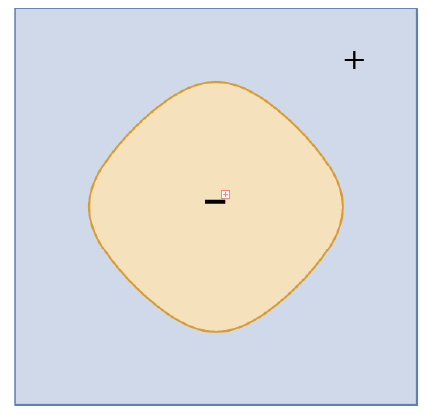
\includegraphics[scale=0.5]{pic/fig11.png}
\caption{BZ中$s_\pm$-波示意图,在靠近中心区域配对是负的,在BZ边界区域配对是正的。}\label{fig10}
\end{figure}
同样的,在$s_\pm$-波配对的情形下,可以来研究低能边界理论,将哈密顿量在$\Gamma=(0,0)$点做展开
\begin{equation}
\begin{aligned}
H(\mathbf{k})&=(m+\frac{t_x}{2}k_x^2+\frac{t_y}{2}k_y^2)\sigma_z\tau_z+\lambda_xk_x\sigma_xs_z+\lambda_yk_y\sigma_y\tau_z\\
&+\left[\Delta_0-2\Delta_1+\frac{\Delta_1}{2}(k_x^2+k_y^2)\right]s_y\tau_y\label{hoti2s}
\end{aligned}
\end{equation}
利用和前面相似的方法,对边界(\uppercase\expandafter{\romannumeral1})将哈密顿量分解为$H=H_0+H_p$
\begin{equation}
\begin{aligned}
H_0(-i\partial_x,k_y)&=(m-t_x\partial_x^2/2)\sigma_z\tau_z-i\lambda_x\sigma_xs_z\partial_x\\
H_p(-i\partial_x,k_y)&=\lambda_yk_y\sigma_y\tau_z+\left[\Delta_0-2\Delta_1-(\Delta_1/2)\partial_x^2\right]s_y\tau_y
\end{aligned}
\end{equation}
$H_0$的四个零能本征解与前面类似,在这四个零能的子空间中$H_p$的有效形式为
\begin{equation}
\begin{aligned}
H_{\mathrm{\uppercase\expandafter{\romannumeral1}}}(k_y)&=-A_yk_ys_z+M_{\mathrm{\uppercase\expandafter{\romannumeral1}}}s_y\tau_y\\
M_{\mathrm{\uppercase\expandafter{\romannumeral1}}}&=\int_{0}^\infty dx\Psi_\alpha^{*}(x)\left[\Delta_0-2\Delta_1-(\Delta_1/2)\partial_x^2\right]\Psi_\alpha(x)\\&=\Delta_0-2\Delta_1-\Delta_1\frac{m}{t_x}
\end{aligned}
\end{equation}
其它边界上的低能有效哈密顿量与(\ref{edge1})类似,$M_{\mathrm{\uppercase\expandafter{\romannumeral3}}}=M_{\mathrm{\uppercase\expandafter{\romannumeral1}}}=\Delta_1m/t_x$,$M_{\mathrm{\uppercase\expandafter{\romannumeral2}}}=M_{\mathrm{\uppercase\expandafter{\romannumeral4}}}$\\$=\int_{0}^{\infty}dy\Psi_\alpha^{*}(y)\left[\Delta_0-2\Delta_1-(\Delta_1/2)\partial^2_y\right]\Psi_\alpha=\Delta_0-2\Delta_1-\Delta_1m/t_y$。利用类似于(\ref{edge2})的边界坐标$l$同样可以得到每条边界上的$A(l)$是相同的,但是Dirac质量项$M(l)$是不一样的,对边界(\uppercase\expandafter{\romannumeral1}),(\uppercase\expandafter{\romannumeral2}),(\uppercase\expandafter{\romannumeral3}),(\uppercase\expandafter{\romannumeral4})其对应的质量项为$M(l)=-\bar{\Delta}_0-\Delta_1m/t_x,-\bar{\Delta
}_0-\Delta_1m/t_y,-\bar{\Delta}_0-\Delta_1m/t_x,-\bar{\Delta}_0-\Delta_1m/t_y$,这里$\bar{\Delta}_0=2\Delta_1-\Delta_0$。

 要保证在每个拐角处都可以形成MKP,那么相邻边上的Dirac质量需要改变符号,即满足下面的条件
\begin{equation}
(\bar{\Delta}_0+\Delta_1m/t_x)(\bar{\Delta}_0+\Delta_1m/t_y)<0\label{ring1}
\end{equation}
定义$R_s\equiv\sqrt{2\bar{\Delta}_0/\Delta_1}$,它代表着超导配对节线的半径,当越过这个节线的时候,配对要变号;$R_x\equiv\sqrt{-2m/t_x},R_y\equiv\sqrt{-2m/t_y}$则表示$m+(t_x/2)k_x^2+(t_y/2)k_y^2=0$(这是能带反转环,即$\sigma_z$项在越过这个环时符号会发生改变)。所以零能模存在条件(\ref{ring1})在化学势$\mu=0$的时候变为
\begin{equation}
(R_s-R_x)(R_s-R_y)<0
\end{equation}
也就意味着此时超导配对节线环需要和能带反转环相交才可以,如图\ref{fig11}所示。
\begin{figure}[h]
\centering
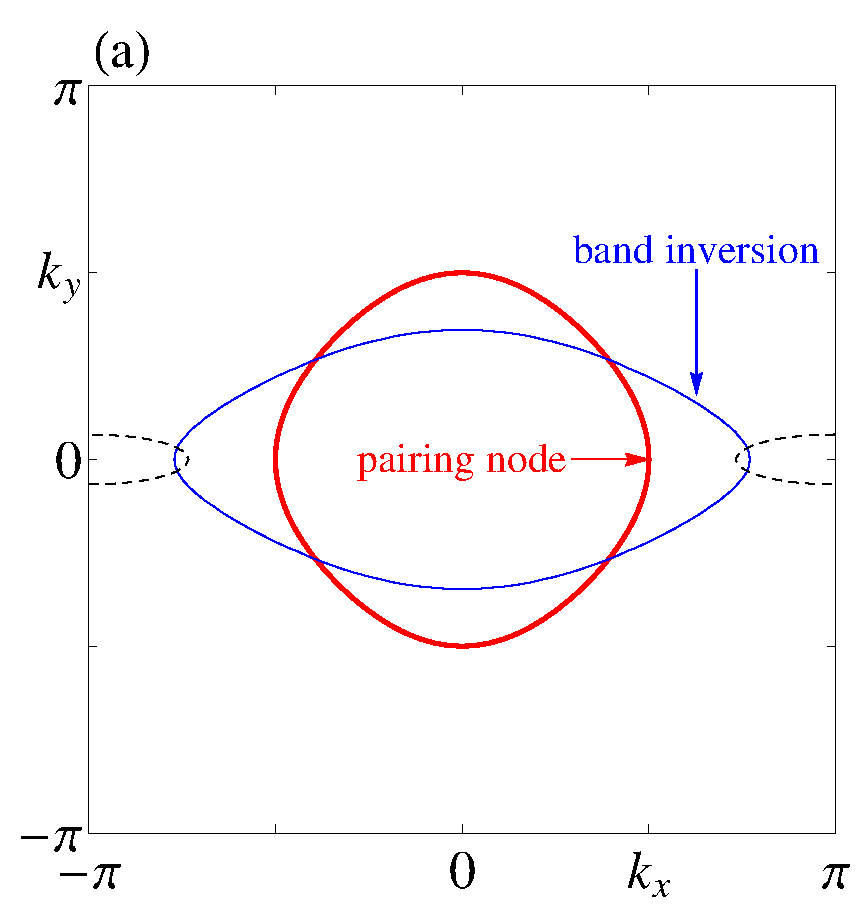
\includegraphics[scale=0.45]{pic/fig12a}
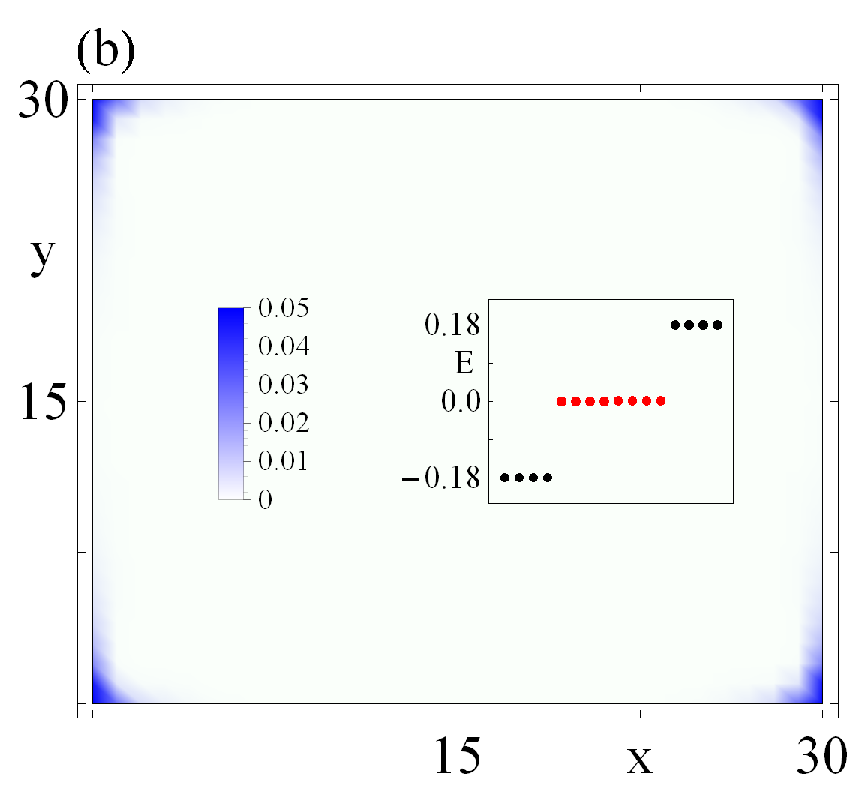
\includegraphics[scale=0.45]{pic/fig12b}
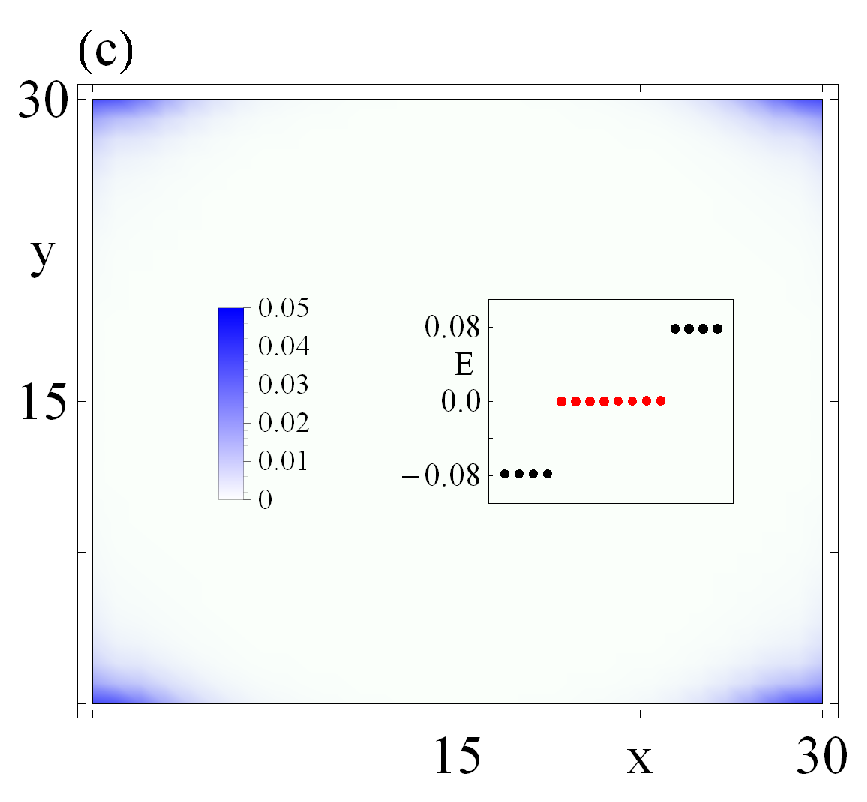
\includegraphics[scale=0.45]{pic/fig12c}
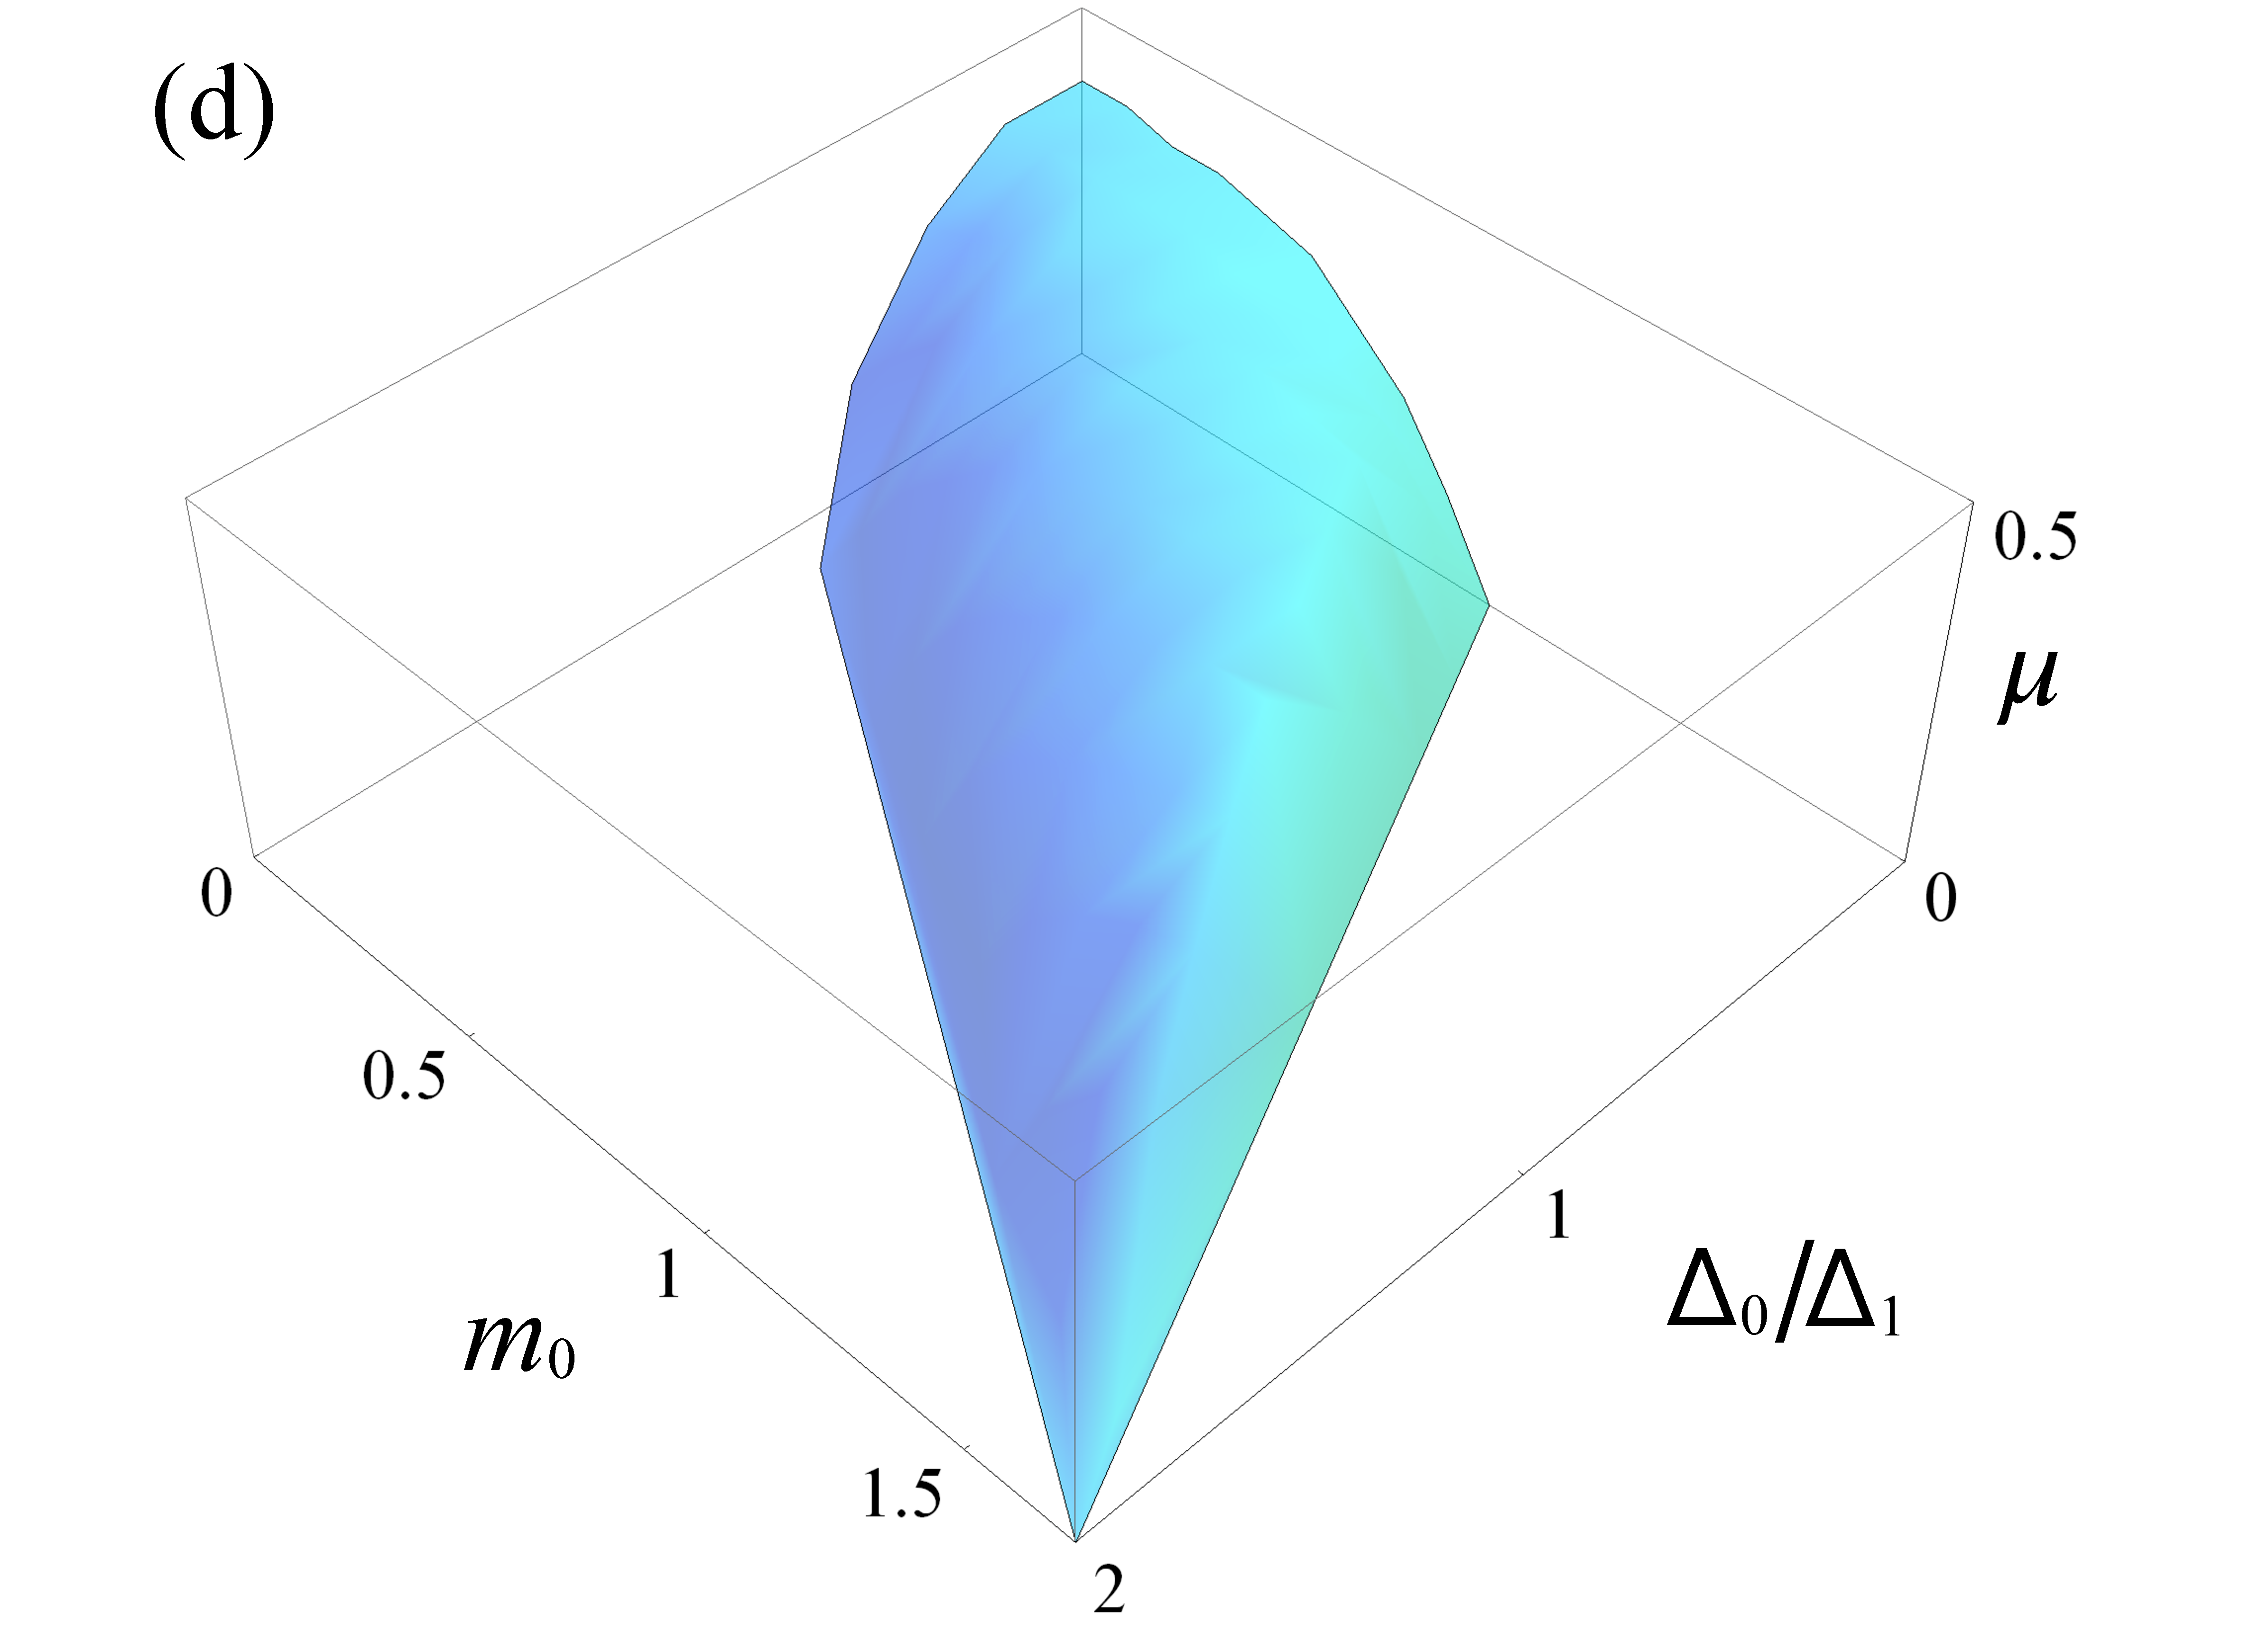
\includegraphics[scale=0.09]{pic/fig12d}
\caption{(a)能带反转环与超导配对节线环,虚线代表着$\mu=0.3$时的费米面;(b-c)零能态波函数分布,(b)中化学势$\mu=0$,(c)中化学势$\mu=0.3$;(d)($m_0,\Delta_0/\Delta_1,\mu$)相图,固定$\Delta_1=0.4$,在表面包括的范围内都可以存在MKP\cite{re28}。}\label{fig11}
\end{figure}

 研究人员还提出了一种利用Rashba自旋轨道耦合,通过超导体的近邻效应在系统中诱导出$s_\pm$-波配对,从而实现高阶拓扑超导体的方案\cite{re27}。
\begin{equation}
\begin{aligned}
H^{\mathrm{BdG}}(\mathbf{k})&=(h^{\mathrm{TI}}(\mathbf{k})-\mu)\tau_z+\Delta(\mathbf{k})\tau_x\\
h^{\mathrm{TI}}(\mathbf{k})&=\left[2t(\cos k_x-\cos k_y)+4t_1\cos k_x\cos k_y\right]\sigma_z+2\lambda(\sin k_xs_y-\sin k_ys_x)\sigma_x\\
\Delta(\mathbf{k})&=\Delta_0+2\Delta_1(\cos k_x+\cos k_y)\label{hosc2}
\end{aligned}
\end{equation}

 在这个方案中,这个模型所描述的2D拓扑绝缘体只有一个能带反转的位置在$(\pi,0)$点,当将哈密顿量沿一个方向取开边界,另外一个方向取周期边界条件的时候,会发现不同的方向开边界其边界态出现的位置是不同,如图\ref{fig12}所示,当沿$y$方向取开边界条件,$x$方向取周期边界的时候,体系的螺旋边界态出现在$k_x=\pi$这个位置处;当沿$x$方向取开边界条件,$y$方向取周期边界的时候,体系的螺旋边界态出现在$k_y=0$这个位置处。当费米面落在体态能隙中间的时候,如果通过近邻效应诱导$s_\pm$-波配对$\Delta(\mathbf{k})=\Delta_0+2\Delta_1(\cos k_x+\cos k_y)$则边界态会被打开一个能隙,当$\Delta_0=0$时结果如图\ref{fig12}(b,d)所示。
\begin{figure}[h]
\centering
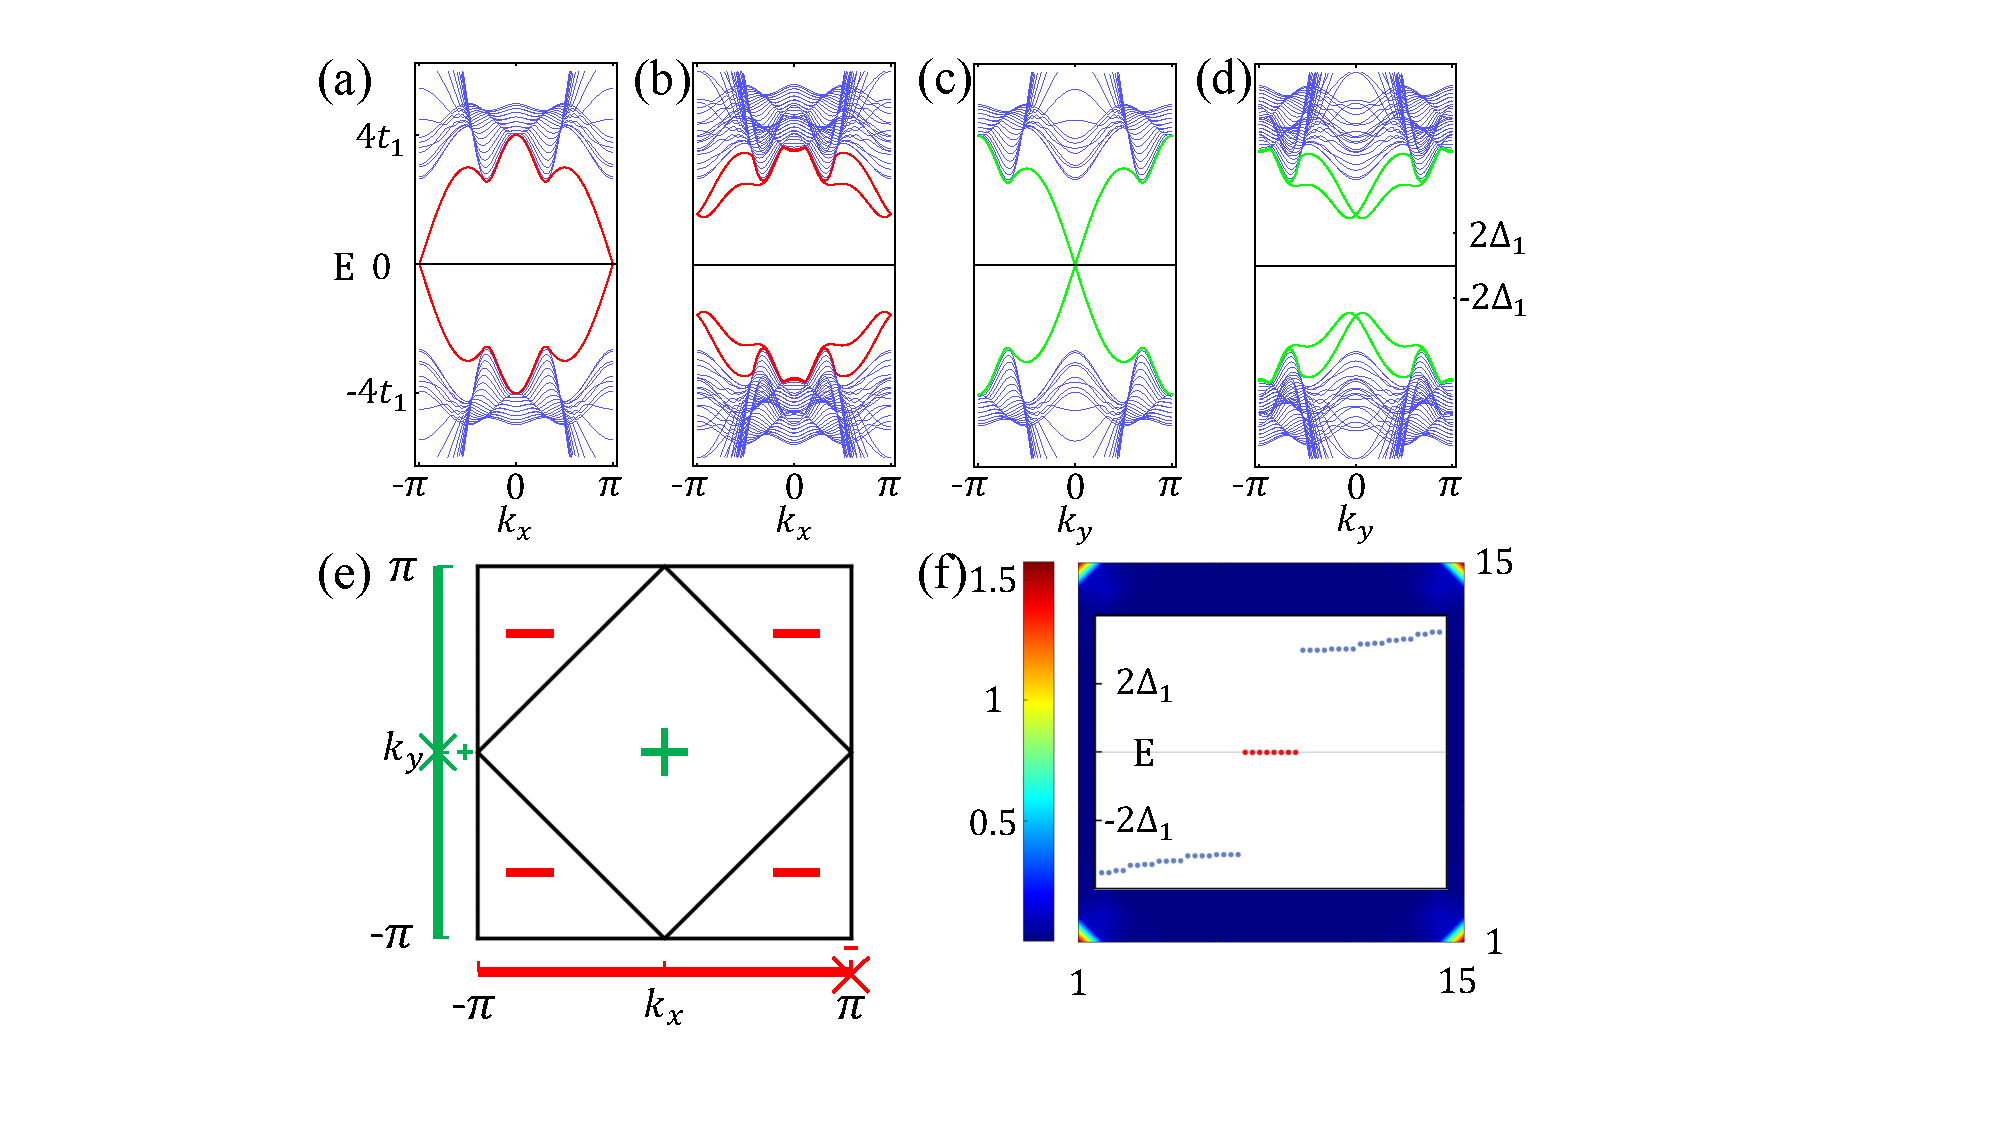
\includegraphics[scale=0.7]{pic/fig13}
\caption{(a)2D拓扑绝缘体沿($0\bar{1}$)方向圆柱体结构能带图,此时边界态出现在$k_x=\pi$;(b)能带(a)在加入$s_\pm$配对后BdG哈密顿量的能谱图;(c-d)和(a-b)相似,此时边界态出现在($\bar{1}0$)这个方向的$k_y=0$处\cite{re27}。}\label{fig12}
\end{figure}
当在一个四方结构的拓扑绝缘体中诱导$s_\pm$-波配对之后,螺旋的边界态会被打开能隙,从而在每个角落处形成马约拉纳卡莱默对,结果如\ref{fig12}(f)所示。

当化学势$\mu$比较小的时候,拐角处局域的马约拉纳卡莱默对可以通过边界分析来解释,如图\ref{fig12}(e)所示,当$\Delta_0=0$的时候,在BZ中超导配对$\Delta(\mathbf{k})$是有正负变化的,在($0\bar{1}$)边界上,$k_x=\pi$处的螺旋边界态所获得的超导配对值为负,因为在$k_x=\pi$处,所有$k_y$对应的$\Delta(\mathbf{k})$都是负号;相反的在$(\bar{1}0)$边界上,$k_y=0$处的边界态所获得的超导配对负号都是正的,因为在$k_y=0$对于所有的$k_x$而言,$\Delta(\mathbf{k})$都是正号。所在这就会在相邻的两个边界处形成质量畴壁,从而在拐角处产生马约拉纳卡莱默对。

除了利用高温超导体电子配对的各向异性来产生高阶拓扑超导体,研究人员同样提出了利用各向同性的$s$-波超导体和一个面内的Zeeman场来实现高阶拓扑超导体\cite{re45}。
\begin{figure}[h]
\centering
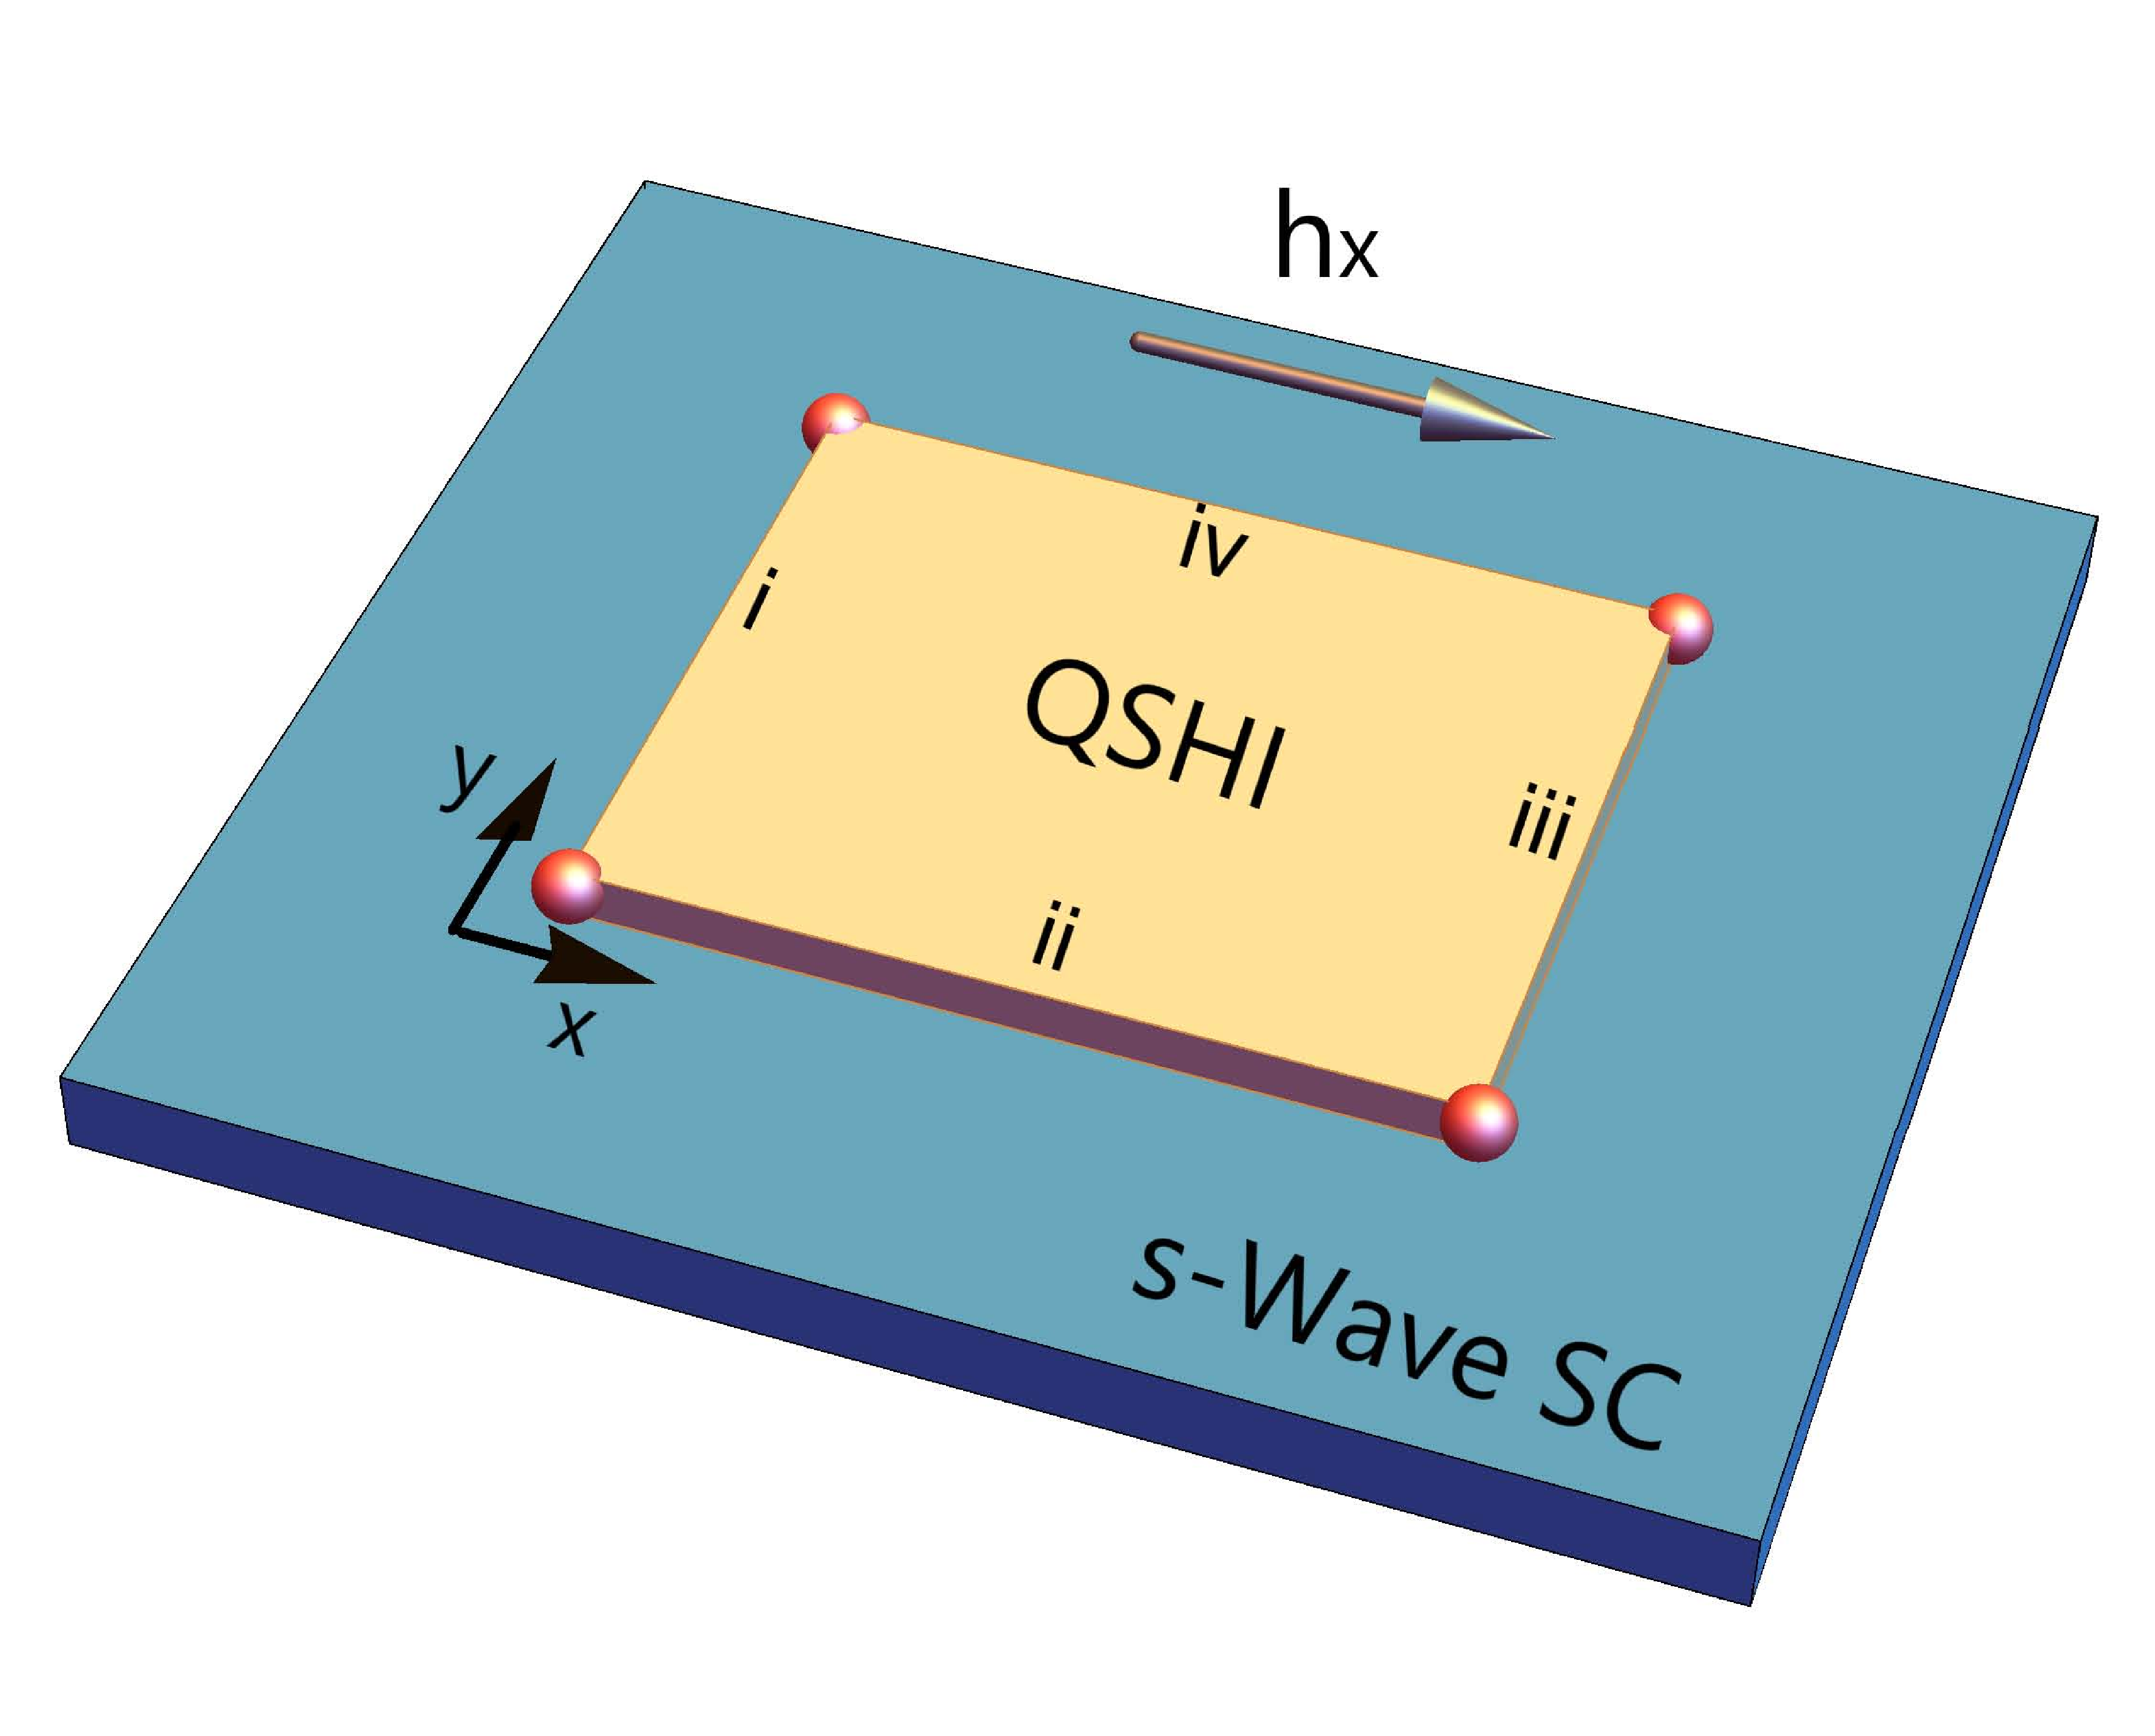
\includegraphics[scale=0.2]{pic/fig14.pdf}
\caption{量子自旋霍尔效应与$s$-波超导构成异质结,并在面内存在一个各项异性的磁场,马约拉纳零能模出现在系统的四个拐角处\cite{re45}。}\label{fig13}
\end{figure}
如示意图\ref{fig13}所示,在$s$-波超导体的基底上放置量子自旋霍尔绝缘体,在面内的$x$方向上存在着Zeeman场,而$y$方向则没有Zeeman,正是这个各向异性的Zeeman场使得不同的边界上诱导出相反的质量,从而可以在系统拐角处产生马约拉纳零能模。由于Zeeman场的存在破坏了时间反演对称,所以此时每个拐角处只有一个马约拉纳零能模。$s$-波超导体相比于其它的高温超导体虽然具有较低的超导转变温度,但是其超导相干长度较大,这一方案在实验上具有更好的实用性。其具体模型为
\begin{equation}
\begin{aligned}
H(\mathbf{k})&=2\lambda_x\sin k_x\sigma_xs_z\tau_z+2\lambda_y\sin k_y\sigma_y\tau_z+(\xi_k\sigma_z-\mu)\tau_z+\Delta_0\tau_x+{\bf h\cdot s}\\
\xi_k&=\epsilon_0-2t_x\cos k_x-2t_y\cos k_y\label{ze1}
\end{aligned}
\end{equation}
可以得到系统低能有效哈密顿量为
\begin{equation}
H_{\textrm{edge},j}=-i\lambda_js_z\tau_z\partial_{l_j}+\Delta_0\tau_x+h_js_x\label{ef2}
\end{equation}
这里的参数为$\lambda_j=\{-2\lambda_y,2\lambda_x,2\lambda_y,-2\lambda_x\},l_j=\{y,x,y,x\},h_j=\{0,h_x,0,h_x\}$。从有效哈密顿量(\ref{ef2})中可以看到,所有的准粒子边界态都存在诱导出的超导序参量,但是Zeeman场并非出现在所有的边界上。而且$\{s_z\tau_z,\tau_x\}=0$,所有的准粒子边界态出现了超导电子配对的质量项,Zeeman场诱导的质量则只是出现在$x$边界上,$y$边界上始终是不存在的。

在利用Zeeman场辅助实现高阶拓扑的这个模型中,各项异性的Zeeman场是重要的原料,而且要满足Zeeman场大于一定值的时候才会在系统拐角处出现马约拉纳零能模。随着Zeeman场逐渐变大,$x$方向上的边界态会经历能隙关闭然后打开能隙,而$y$方向上的边界态始终是无能隙的,边界态经历能隙关闭并打开的过程,正对应着拓扑相变,从而就会在边界的边界上(拐角)形成零能的束缚态。这种边界态经历相变从而实现的高阶拓扑相被称为边界阻塞拓扑相\cite{re46}。
\subsection{异质结系统中的超导近邻效应}
 在实现高阶拓扑超导的方案中,通常都需要用到异质结结构\cite{re27,re28,re29,re34,re38,re39,re45}。在异质结系统中,与超导体相近邻的系统的表面上同样会被诱导出电子配对,这就是超导
的近邻效应。在之前利用异质结结构研究高阶拓扑超导的研究中,近邻效应只是被唯象的考虑,即在模型中直接加入一个有效的电子配对,忽略了不同层能带之间的混合\cite{re27,re28,re29,re34,re38,re39,re45}。然而在实际中,对于一个混合体系,一个更加微观的模型应该同时考虑不同体系的原始哈密顿量,而且需要考虑它们之间的耦合。非超导层的电子配对应该是由层间电子隧穿诱导出来的。这样的一个微观模型已经在研究一阶拓扑超导的方案中受到关注,很多不同现象被发现\cite{re47,re48,re49,re50,re51,re52,re53,re54,re55}。特别注意的是,研究人员发现在近邻层诱导出的超导配对对称性与超导层的会不一致\cite{re48,re49}。

 在Be$_2$Se$_3$与Bi$_2$Sr$_2$CaCu$_2$O$_{8+\delta}$(BSCCO)的异质结中系统中,Yao等人\cite{re48}通过微观模型在平均场的层面研究了BSCCO在Bi$_2$Se$_3$中诱导的电子配对大小,模型设置及结果如图\ref{fig14}所示
\begin{figure}[h]
	\centering
	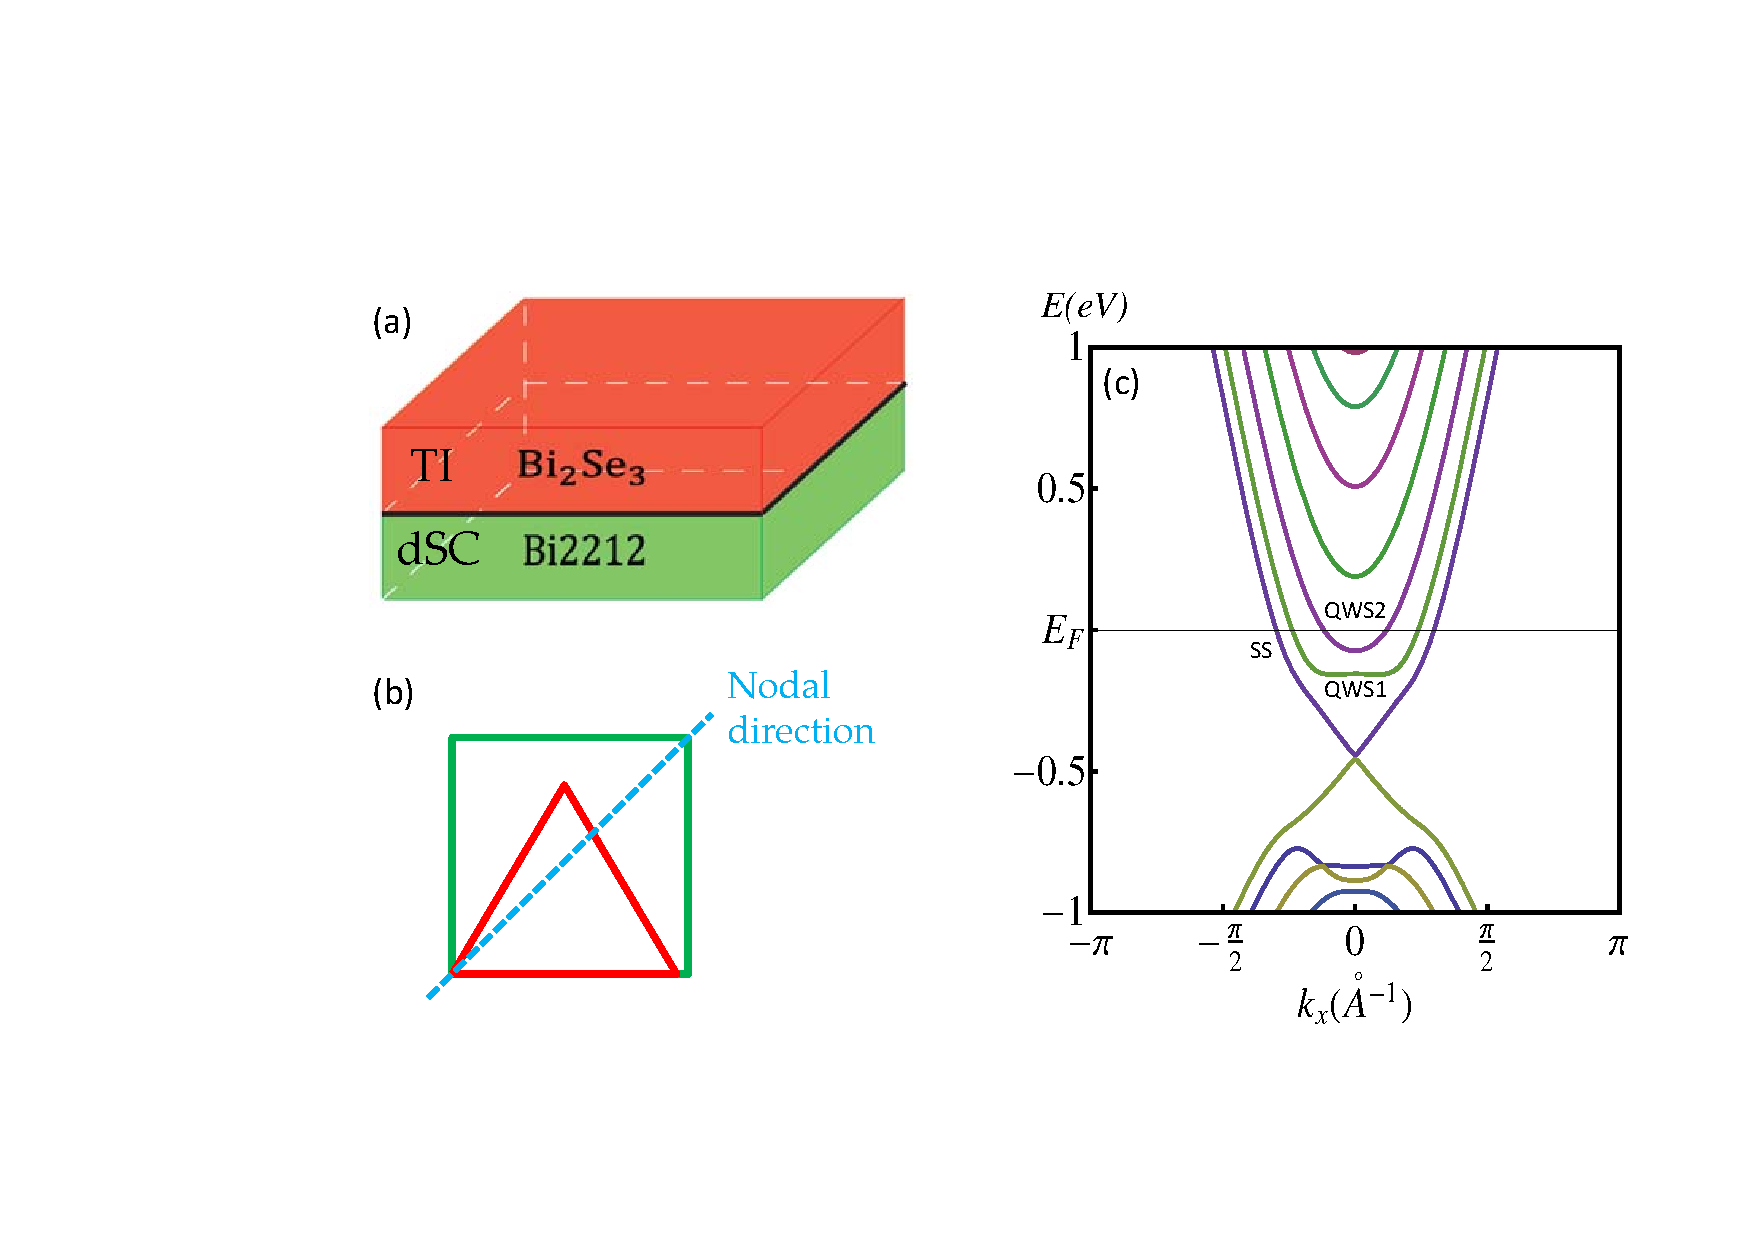
\includegraphics[scale=0.7]{pic/fig15.pdf}
	\caption{(a)拓扑绝缘体/高温超导体异质结。(b)Bi$_2$Se$_3$与BSCCO的相对晶格取向,沿着超导配对节线方向,体系波坏了$90^\circ$旋转和反射对称。(c)拓扑绝缘体Bi$_2$Se$_3$的能带结构\cite{re48}。}\label{fig14}
\end{figure}
铜基超导电子配对是$d$-波配对,旋转$90^\circ$或者沿着$x^{'}z$($x^{'}\sim \hat{x}+\hat{y}$)反射后是奇函数。如果拓扑绝缘体Be$_2$Se$_3$同样满足这样的条件,那么在其表面上诱导出的电子配对一定会存在$d$-波配对形式,而不会存在$s$-波形式的电子配对。所以在拓扑绝缘体表面上诱导出的电子配对就会存在节点。但是拓扑绝缘体Be$_2$Se$_3$的晶体结构并不满足这样的对称要求,异质结中两层材料之间晶体结构的不匹配导致有可能在Be$_2$Se$_3$表面上诱导出有限大小的$s$-波配对,从而在拓扑绝缘体的表面上可以同时存在$d$-波配对和$s$-波配对。随着拓扑绝缘体化学势的变化,体系的费米面形状也会随之改变,当费米面较小的时候,对于$d$-波这种各项异性较强的配对,其贡献就可以忽略,从而使得各项同性的$s$-波配对占主导。
%=================================================================
\subsection{本章总结}
 本章主要介绍了通常的一阶拓扑相和高阶拓扑相的基本概念,并介绍了在理论上通过拓扑绝缘体和高温超导体异质结来实现高阶拓扑超导体的方案,并介绍了有效边界理论分析了高阶拓扑中拐角态的起源。而且通过不同的拓扑绝缘体模型,所需要的超导电子配对的形式也有所不同。之后又介绍了利用常规的$s$-波超导体外加一个面内的Zeeman场来实现高阶拓扑超导体,探寻马约拉纳拐角态的理论模型,这都为之后的实验涉及与理论研究奠定了一定的基础。最后通过对异质结中近邻效应的介绍,说明在这种结构中,近邻效应诱导的电子配对形式是多组分的,在真实的实验体系中,当不同配对组分之间比重相差不大时,并不能简单的通过唯象方式仅仅关心其中的某一种配对形式,这也给出了本论文的主要研究方向。











\newpage
\section{第二章\quad 模型建立}
%\setcounter{page}{1}
%\pagestyle{plain}
\subsection{引言}
 通过前面的介绍,可以发现高阶拓扑超导体相对于传统的一阶拓扑超导具有不一样的特性:在比体系维度低2维或者3维的边界上存在束缚态,且这些束缚态是受拓扑保护的马约拉纳零能态。为了实现高阶拓扑超导体,研究人员提出的主要方案是利用超导体的近邻效应与拓扑绝缘体构成异质结结构,这个方案最初提出是通过近邻效应在3D拓扑绝缘体的表面态上诱导$s$-波配对,由于自旋轨道耦合的存在,可以在表面上形成等效的$p$-波超导体。理论上研究表明,在$p\pm ip$超导体的vortex中会束缚马约拉纳费米子,可以用来实现拓扑量子计算。在高阶拓扑超导体中,同样在拓扑绝缘体中利用近邻效应在其中诱导超导配对,此时需要的是转变温度较高的高温超导体,其配对形式相比于$s$-波而言具有各向异性,从而可以在不同的方向上诱导出相反质量的畴壁,从而可以在质量相反的交界处形成马约拉纳零能模。在前面的利用近邻效应研究高阶拓扑的模型中,超导配对被视为拓扑绝缘体的本征属性,直接加入到了拓扑绝缘体的哈密顿量中,忽略了异质结结构不同层之间的能带混合。

 之前的研究结果也表明通过近邻效应诱导的超导电子配对形式与超导层电子配对的形式并不是完全相同的\cite{re48,re49},那么在利用近邻效应产生高阶拓扑超导体时,异质结不同层之间的耦合也是不容忽略的。本论文中,在前面提出研究高阶拓扑超导体的模型\cite{re27,re28,re29}的基础上,我考虑了一个2D拓扑绝缘体和$d$-波超导体异质结结构,并考虑了拓扑绝缘体与超导体之间的层间耦合作用,通过这个微观模型来研究高阶拓扑超导体中的马约拉纳拐角态。
%============================================
\subsection{模型与哈密顿量}
 异质结结构在研究不同材料之间性能结合方面具有很广泛的应用,在通过微观模型研究这样的系统时,通常需要独立考虑两层之间各自的哈密顿量,并考虑两层之间的耦合,通常最简单的耦合方式是考虑两层之间电子的隧穿跃迁。

 本论文研究中考虑最简单的层间跃迁耦合,我们给出一个考虑2D拓扑绝缘体与$d$-波超导体的两层系统,它的微观模型哈密顿量为
\begin{equation}
H=H_\mathrm{TI}+H_\mathrm{SC}+H_\mathrm{I}\label{ham}
\end{equation}
$H_\mathrm{TI}$是正方格点上的2D拓扑绝缘体层的哈密顿量\cite{re56,re57},
\begin{equation}
\begin{aligned}
H_{TI} =\sum_{{\bf k}}C_{{\bf k}}^\dagger (h_\mathbf{k}\sigma_3s_0+2\lambda_{0}\sin k_x\sigma_1s_3+2\lambda_0\sin k_y\sigma_2 s_0)C_{{\bf k}},
\end{aligned}
\end{equation}
这里$h_\mathbf{k}=h_0-2t(\cos k_x+\cos k_y)$,矢量$C^\dagger_{\bf k}$ 可以表示为$C^\dagger_{\bf k}=(c^\dagger_{{\bf k}1\uparrow},c^\dagger_{{\bf k}2\uparrow},c^\dagger_{{\bf k}1\downarrow},c^\dagger_{{\bf k}2\downarrow})$,这里下表$1,2$和$\uparrow,\downarrow$分别代表的是轨道与自旋索引。$s_i$与$\sigma_i$分别代表的是自旋空间和轨道空间的单位矩阵($i=0$)或者泡里矩阵($i=1,2,3$)。

 $H_\mathrm{SC}$描述一个$d$-波超导体
\begin{equation}
H_{SC}=\sum_{{\bf k}\sigma}\varepsilon_{\bf k}d^\dagger_{{\bf k}\sigma}d_{{\bf k}\sigma}+\sum_{{\bf k}}\Delta_{\bf k}(d^\dagger_{{\bf k}\uparrow}d^\dagger_{{-\bf k}\downarrow}+h.c.),
\end{equation}
这里 $\varepsilon_{\bf k}=-2t(\cos k_x+\cos k_y)-\mu$, 动量空间中的超导配对为 $\Delta_{\bf k}=2\Delta_0 (\cos k_x-\cos k_y)$.

\qquad $H_\mathrm{I}$描述的是超导层与2D拓扑绝缘体层之间的单粒子跃迁项
\begin{equation}
H_{I}=-t_\perp \sum_{{\bf k}\tau\sigma}(c_{{\bf k}\tau\sigma}^\dagger d_{{\bf k}\sigma}+h.c.).
\end{equation}

 为了研究边界条件,我们通常习惯对哈密顿量考虑一个圆柱体结构,如图\ref{fig15}所示,即在某一个方向上的尺寸是有限的,另外一个方向是周期的,这样有限尺寸方向的平移对称性被破坏。这种情况下只需要对哈密顿量沿这个方向做傅里叶变换。
\begin{figure}
\centering
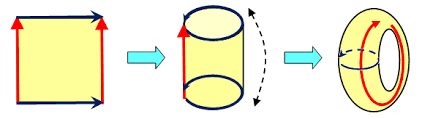
\includegraphics[scale=0.6]{pic/fig16}
\caption{圆柱形结构示意图}\label{fig15}
\end{figure}


 比如,我们考虑沿$y$方向取开边界条件,哈密顿量可以表示为
\begin{equation}
	\begin{aligned}
		H_{TI} &= \sum_{y,k_x}C^\dagger_{y}(k_x)[(h_0-2t\cos k_x)\sigma_3s_0 \\&+2\lambda_0\sin k_x\sigma_1s_0]C_{y}(k_x)
		+\sum_{y,k_x}[C^\dagger_{y}(k_x)\\&(-t\sigma_3s_0-i\lambda_0\sigma_2s_3)C_{y+1}(k_x)+h.c],
	\end{aligned}
\end{equation}

\begin{equation}
	\begin{aligned}
		H_{SC} &= \sum_{y,k_x,\sigma}d^\dagger_{y\sigma}(k_x)(-2t\cos k_x -\mu)d_{y\sigma}(k_x)\\
		&+\sum_{y,k_x}[d^\dagger_{y\uparrow}(k_x)(-2\Delta_0\cos k_x)d^\dagger_{y\downarrow}(-k_x)+h.c]
		\\&-t\sum_{y,k_x,\sigma}[d^\dagger_{y\sigma}(k_x)d_{y+1,\sigma}(k_x)+h.c]\\
		&+\Delta_0\sum_{y,k_x}[d^\dagger_{y\uparrow}(k_x)d^\dagger_{y+1,\downarrow}(-k_x)+h.c],
	\end{aligned}
\end{equation}
\begin{equation}
	H_I=-t_\perp\sum_{y,k_x,\alpha,\sigma}[c^\dagger_{y\alpha\sigma}(k_x)d_{y\sigma}(k_x)+h.c].
\end{equation}
 为了在实空间数值的研究马约拉纳拐角态,我们需要同时在$x$与$y$方向上取开边界条件。在这种情况下,哈密顿量在实空间的表达形式为
\begin{equation}
	\begin{aligned}
		H_{TI} &=-t\sum_{{\bf i}\alpha}(C_{{\bf i}}^\dagger \sigma_3s_0   C_{{\bf i}+\hat{\alpha}}+h.c.)+h_0\sum_{{\bf i}\tau}C_{{\bf i}}^\dagger \sigma_3s_0   C_{{\bf i}}
		\\&-\lambda_0\sum_{{\bf i}}(iC_{{\bf i}}^\dagger\sigma_1s_3C_{{\bf i}+\hat{x}}-iC_{{\bf i}}^\dagger\sigma_2s_0C_{{\bf i}+\hat{y}}+h.c.),
	\end{aligned}
\end{equation}
\begin{equation}
	\begin{aligned}
		H_{sc} &=-t\sum_{{\bf i}\alpha\sigma}(d_{{\bf i}\sigma}^\dagger d_{{\bf i}+\hat{\alpha},\sigma}+h.c.)-\mu\sum_{{\bf i}\sigma}d_{{\bf i}\sigma}^\dagger d_{{\bf i}\sigma}
		\\&+\sum_{\langle{\bf ij}\rangle}(\Delta_{\bf ij}d_{{\bf i}\uparrow}^\dagger d_{{\bf j}\downarrow}^\dagger+h.c.),
	\end{aligned}
\end{equation}

\begin{equation}
	H_{I}=-t_\perp \sum_{{\bf i}\tau\sigma}(c_{{\bf i}\tau\sigma}^\dagger d_{{\bf i}\sigma}+h.c.),
\end{equation}
对于$d$-波超导体配对,格点$\mathbf{j}$代表着格点$\mathbf{i}$的最近邻位置,$\Delta_\mathbf{ij}=\pm\Delta_0$,由于$d$-波配对$\pm$号依赖于$\langle\mathbf{ij}\rangle$是沿着$x$方向还是$y$方向。

 整个的哈密顿量可以被写成矩阵形式。在动量空间中它是一个$12\times 12$的矩阵$\hat{M}$,$H=\sum_{\mathbf{k}}\Psi_\mathbf{k}^\dagger\hat{M}\Psi_\mathbf{k}$。这里矢量$\Psi^\dagger_\mathbf{k}$表示为
\begin{equation}
\Psi^\dagger_{\bf k}=(C^\dagger_{\bf k},C_{-{\bf k}},d^\dagger_{{\bf k}\uparrow},d^\dagger_{{\bf k}\downarrow},d_{-{\bf k}\uparrow},d_{-{\bf k}\downarrow}).
\end{equation}
哈密顿量的矩阵形式$\hat{M}$可以表示为
\begin{equation}
\left[
\begin{array}{ccc}
M^{TI}(\mathbf{k}) & \mathbf{0}_{4\times 4} &M_1 \\
\mathbf{0}_{4\times 4} & -M^{TI}(\mathbf{-k}) & M_2 \\
M^{\dagger}_1 & M^{\dagger}_2 & M^{SC}(\mathbf{k})
\end{array}
\right],
\end{equation}
这里
\begin{equation}
M^{TI}(\mathbf{k})=\left[
\begin{array}{cccc}
h({\mathbf{k}}) & \lambda(\mathbf{k}) & 0 & 0 \\
\lambda(\mathbf{k})^* & -h({\mathbf{k}}) & 0 & 0 \\
0 & 0 & h({\mathbf{k}}) & -\lambda(\mathbf{k})^* \\
0 & 0 & -\lambda(\mathbf{k})^\dagger & -h({\mathbf{k}}),
\end{array}
\right]
\end{equation}
取 $\lambda(\mathbf{k})= 2\lambda_0\sin k_x- 2i\lambda_0\sin k_y$.

\begin{equation}
M^{SC}(\mathbf{k})=
\left[
\begin{array}{cccc}
\epsilon({\mathbf{k}}) & 0 & 0 & \Delta(\mathbf{k}) \\
0 & \epsilon({\mathbf{k}}) & -\Delta(\mathbf{k}) & 0 \\
0 & -\Delta(\mathbf{k}) & -\epsilon({\mathbf{k}}) & 0 \\
\Delta(\mathbf{k}) & 0 & 0 & -\epsilon({\mathbf{k}})
\end{array}
\right],
\end{equation}
\begin{equation}
M_1=-t_{\perp}\left[
\begin{array}{cccc}
1 & 0 & 0 & 0 \\
1 & 0 & 0 & 0 \\
0 & 1 & 0 & 0 \\
0 & 1 & 0 & 0
\end{array}
\right],\quad
M_2=-t_{\perp}\left[
\begin{array}{cccc}
0 & 0 & -1 & 0 \\
0 & 0 & -1 & 0 \\
0 & 0 & 0 & -1 \\
0 & 0 & 0 & -1
\end{array}
\right].
\end{equation}
在一个圆柱体结构且沿$y$方向取开边界条件,此时整个哈密顿量可以被写为$12N_y\times 12N_y$的矩阵形式$H=\sum_{k_x}\Psi^\dagger(k_x)\hat{M}(k_x)\Psi(k_x)$。$N_y$是沿$y$方向取开边界条件时所取的格点数目。矢量$\Psi^\dagger(k_x)$可以表示为
\begin{equation}
\Psi^\dagger(k_{x}) =(C^\dagger_1(k_x),C_{1}(k_x),\cdots,C^\dagger_{N_y}(k_x),C_{N_y}(k_x),d^\dagger_{1\uparrow}(k_x),\cdots,d_{N_y\downarrow}(k_x)).\label{b1}
\end{equation}

 在实空间中,哈密顿量矩阵$\hat{M}$大小为$N\times N$,这里$N=8N_1+4N_2$,$N_1,N_2$分别是实空间中2D拓扑绝缘体和$d$-波超导体的格点数目。矢量$\Psi^\dagger$表示为
\begin{eqnarray}
\Psi^\dagger =(C^\dagger_1,C_{1},\cdots,C^\dagger_{N_1},C_{N_1},d^\dagger_{1\uparrow},\cdots,d_{N_2\downarrow}).\label{b2}
\end{eqnarray}
方程(\ref{b1})中的矢量$C^\dagger_i(k_x)$和方程(\ref{b2})中的$C^\dagger_i$是矢量$C^\dagger_\mathbf{k}$的傅里叶变换。

 通过对哈密顿量矩阵进行对角化,我们可以得到推迟格林函数矩阵$\hat{G}$,其矩阵元表示为
\begin{equation}
G_{ij}(E)=\sum_n\frac{u_{in}u^{*}_{jn}}{E-E_n+i\Gamma}.
\end{equation}
这里$u_{in}$ 和 $E_n$分别代表着矩阵的本征矢量和本征值。

 在动量空间中,2D拓扑绝缘体层的谱函数可以通过格林函数计算
\begin{equation}
A({\bf k},E)=-\frac{1}{\pi}\sum^4_{p=1}\mathrm{Im} G_{pp}({\bf k},E).
\end{equation}

\qquad 对于一个圆柱体结构,谱函数可以通过下面公式计算
\begin{equation}
A_{y}(k_{x},\omega)=-\frac{1}{\pi}\sum_{p=1}^{4}\mathrm{Im} G_{m+p,m+p}(k_x,\omega),
\end{equation}
这里 $m = 8(i_y-1)$。

 对于轨道$\mathbf{\tau}$通过近邻效应诱导的配对项可以通过平均场序参量来研究,表达为
\begin{equation}
\Delta_\tau({\bf k})=\langle c^\dagger_{{\bf k}\tau\uparrow}c^\dagger_{-{\bf k}\tau\downarrow}\rangle=\sum_n{u^{*}_{\tau,n}({\bf k})u_{\tau+6,n}({\bf k})}f(E_n),
\end{equation}
这里$f(x)$代表费米分布函数。

 在实空间中,轨道$\mathbf{\tau}在$格点$i$和$j$上的有效配对序参量表达式为
\begin{equation}
\Delta^\tau_{ij}=\sum_nu^{*}_{h(i),n}u_{h(j)+6,n}f(E_n),
\end{equation}
这里 $h(i)=\tau+8(i-1)$。

 我们可以对轨道$\mathbf{\tau}$定义一个位置以来的$d$-波配对
\begin{equation}
\Delta^\tau_i=\mid \Delta^\tau_{i,i+\hat{x}}+\Delta^\tau_{i,i-\hat{x}}
-\Delta^\tau_{i,i+\hat{y}}-\Delta^\tau_{i,i-\hat{y}}\mid.
\end{equation}
在系统的边界上,$\Delta_i^\tau$表示为
\begin{equation}
\Delta^\tau_i=\mid 2(\Delta^\tau_{i,i+\hat{\alpha}}+\Delta^\tau_{i,i-\hat{\alpha}}) \mid  \qquad (\alpha=x,y).
\end{equation}

 在2D拓扑绝缘体的格点$i$上的局域电子态密度(LDOS)可以通过实空间中的格林函数计算
\begin{equation}
\rho_i(E)=-\frac{1}{\pi}\sum^4_{p=1}\mathrm{Im} G_{m+p,m+p}(E).
\end{equation}
这里 $m=8(i-1)$。

 在接下来的计算中,我们取跃迁常数$t$作为能量单位(从高温超导体的带宽可以估计出$t=0.17eV$),其他的参数设置如下;$\lambda_0=0.5$, $h_0=3$, $\mu=-0.3$, $\Delta_0=0.2$, $t_\perp=0.8$,$\Gamma=0.01$.
%============================================
\subsection{运动方程}
\qquad 对任意两个算符$A$与$B$组成的函数,在海森堡绘景中
\begin{equation}
\begin{aligned}
G_r(t,t^{'})&=-\frac{i}{\hbar}\theta(t-t^{'})\langle\left[A(t),B(t^{'})\right]_\pm\rangle\\
&=\left\{
\begin{array}{cc}
-\frac{i}{\hbar}(\langle A(t)B(t^{'})\rangle\pm\langle B(t^{'})A(t)\rangle)\quad (t>t^{'})\\
0\quad(t<t^{'})
\end{array}
\right.\\
&=\langle\langle A(t);B(t^{'})\rangle\rangle_r\label{eom1}
\end{aligned}
\end{equation}
这里泊松括号的下标$\pm$是为了方便这样标记的,当$A$与$B$是费米子型算符时,满足反对易关系,此时取$+$号,而对于玻色子型算符,则满足对易关系,此时取$-$号。在公式(\ref{eom1})中$\langle\dots\rangle$代表统计平均,对于正则系综
\begin{equation}
\langle A\rangle=Z^{-1}\mathrm{Tr}(e^{-\beta H}A),\quad Z=\mathrm{Tr}(e^{-\beta H}),\quad\beta=(k_BT)^{-1}
\end{equation}
由于算符乘积就迹具有轮换不变性
\begin{equation}
\mathrm{Tr}(ABC)=\mathrm{Tr}(CAB)=\mathrm{Tr}(BCA)
\end{equation}
则可以推导出
\begin{equation}
\begin{aligned}
\langle A(t)B(t^{'})\rangle&=Z^{-1}\mathrm{Tr}(E^{-\beta H}e^{\frac{i}{\hbar}Ht}Ae^{-\frac{i}{\hbar}H(t-t^{'})}Be^{-\frac{i}{\hbar}Ht^{'}})\\
&=Z^{-1}\mathrm{Tr}(e^{-\beta H}e^{\frac{i}{\hbar}H(t-t^{'})}Ae^{-\frac{i}{\hbar}H(t-t^{'})}B)\\
&=Z^{-1}\mathrm{Tr}\left[e^{-\beta H}A(t-t^{'})B\right]\\
&=\langle A(t-t^{'})B(0)\rangle
\end{aligned}
\end{equation}
同理也可以证明
\begin{equation}
\langle B(t^{'}A(t))\rangle=\langle B(0)A(t-t^{'})\rangle
\end{equation}
于是双时格林函为
\begin{equation}
\begin{aligned}
G_r(t,t^{'})&=-\frac{i}{\hbar}\theta(t-t^{'})\langle\left[A(t),B(t^{'})\right]_\pm\rangle\\
&=-\frac{i}{\hbar}\langle\left[A(t-t^{'}),B(0)\right]_\pm\\
&=G_r(t-t^{'})
\end{aligned}
\end{equation}
这说明$G_r$只是时间差$(t-t^{'})$的函数。我们可以简单的令$t^{'}=0$,并令$t$代表时间差,则格林函数的定义就可以简化为
\begin{equation}
G_r(t)\equiv\langle\langle A(t);B\rangle\rangle_r=-\frac{i}{\hbar}\theta(t)\langle\left[A(t),B\right]_\pm\rangle\label{gf1}
\end{equation}
其中$B=B(0)$,而
\begin{equation}
A(t)=e^{\frac{i}{\hbar}H t}Ae^{-\frac{i}{\hbar }H t}
\end{equation}
$G_r(t)$的傅里叶变换为
\begin{equation}
G_r(t)=\frac{1}{2\pi}\int_{-\infty}^{\infty}d\omega G_r(\omega)e^{-i(\omega+i\eta)t}\qquad(\eta=+0)
\end{equation}
其逆变换为
\begin{equation}
G_r(\omega)=\int_{-\infty}^{\infty}dtG_r(t)e^{i(\omega+i\eta)t}\equiv\langle\langle A|B\rangle\rangle_{\omega+i\eta}\label{gr}
\end{equation}
在实际的运算中,更多讨论的是格林函数$G_r(\omega)$的性质。

 对于有限温度,各种本征态$|n\rangle$均以概率$Z^{-1}e^{-\beta E_n}$出现,此时公式(\ref{gf1})中的$\langle(\dots)\rangle$不再是基态平均$\langle n|(\dots)|n\rangle$,而应该取统计平均$Z^{-1}\sum_ne^{-\beta E_n}\langle n|(\dots)|n\rangle$,则可以将(\ref{gf1})表示为
\begin{equation}
-\frac{i}{\hbar}\theta(t)Z^{-1}\sum_{n,m}e^{-\beta E_n}\{\langle n|A|m\rangle\langle m|B|\rangle e^{i\omega_{nm}t}\pm\langle n|B|m\rangle\langle m|A|n\rangle e^{-i\omega_{nm}t}\}
\end{equation}
其中$\omega_{nm}\equiv(E_n-E_m)$,再对上式中的第一项做变量替换$n\leftrightarrow m$,即可以得到温度$T>0$时的$G_r(t)$为
\begin{equation}
G_r(t)=-\frac{i}{\hbar}\theta(t)Z^{-1}\sum_{n,m}e^{-\beta E_n}\langle n|B|m\rangle\langle m|A|n\rangle\times e^{-\frac{i}{\hbar}(E_n-E_m)t}(e^{\beta(E_n-E_m)}\pm 1)\label{gf2}
\end{equation}
通过对(\ref{gf2})做傅里叶变换,即可得到频率空间的表示
\begin{equation}
\begin{aligned}
G_r(\omega)&=Z^{-1}\sum_{n,m}e^{-\beta E_n}\langle n|B|m\rangle\langle m|A|n\rangle\times\frac{e^{\beta(E_n-E_m)}\pm 1}{\hbar\omega-(E_n-E_m)+i\eta}\\
&\equiv\langle\langle A|B\rangle\rangle_{\omega+i\eta}\label{gf3}
\end{aligned}
\end{equation}
谱函数表示为
\begin{equation}
\begin{aligned}
A(\omega)&\equiv-\frac{1}{\pi}\mathrm{Im}G_r(\omega)\\
&=Z^{-1}\sum_{n,m}e^{-\beta E_n}\langle n|B|m\rangle\langle  m|A|n\rangle(e^{\beta\hbar\omega_{nm}}\pm 1)\delta\left[\hbar\omega-(E_n-E_m)\right]\\
&=Z^{-1}\sum_{n,m}\langle n|B|m\rangle\langle  m|A|n\rangle(e^{-\beta E_m}\pm e^{-\beta E_n})\delta\left[\hbar\omega-(E_n-E_m)\right]
\end{aligned}
\end{equation}

 推迟格林函数$\langle\langle A|B\rangle\rangle_{\omega+i\eta}$的极点在下半复平面,它只是上半复平面的解析函数,如果将(\ref{gr})中的$i\eta$换成$-i\eta$则可以定义一个在下半复平面的解析函数
\begin{equation}
\langle\langle A|B\rangle\rangle_{\omega-i\eta}\equiv Z^{-1}\sum_{n,m}e^{-\beta E_n}\langle n|B|m\rangle\langle m|A|n\rangle\times \frac{e^{\beta(E_n-E_m)}\pm 1}{\hbar\omega-(E_n-E_m)-i\eta}=G_a(\omega)\label{gf4}
\end{equation}
它的极点在上半平面,再对$G_a(\omega)$做傅里叶变换
\begin{equation}
\begin{aligned}
G_a(t)&=\frac{1}{2\pi}\int_{-\infty}^{\infty}d\omega G_a(\omega)e^{-i(\omega-i\eta)t}\quad(\eta=+0)\\
&=-\frac{i}{\hbar}\theta(-t)\langle\left[A(t),B\right]_\pm\rangle\equiv\langle\langle A(t);B\rangle\rangle_a\\
&=\left\{
\begin{array}{cc}
0\qquad(t>0)\\
\frac{i}{\hbar}\{\langle A(t)B\rangle\pm\langle BA(t)\rangle\}\qquad(t<0)
\end{array}
\right.
\end{aligned}
\end{equation}
这里所求的的时间关联函数是逆时序传播的,代表超前格林函数,因此用$G_a(t)$与$G_a(\omega)$表示。

 利用$G_r(\omega)$与$G_a(\omega)$可以定义包含上、下半复平面在内的全格林函数
\begin{equation}
\begin{aligned}
G(\omega)&\equiv\langle\langle A|B\rangle\rangle_\omega\\
&=Z^{-1}\sum_{n,m}e^{-\beta E_n}\langle n|B|m\rangle\langle m|A|n\rangle\frac{e^{\beta(E_n-E_m)}\pm 1}{\hbar\omega-(E_n-E_m)}\\
&=\left\{
\begin{array}{cc}
G_r(\omega)\qquad(\textrm{上半复平面})\\
G_a(\omega)\qquad(\textrm{下半复平面})
\end{array}\right.\label{gf5}
\end{aligned}
\end{equation}
这里$\omega$为复量。

 利用公式(\ref{gf5})中定义的全格林函数$G(\omega)$,做傅里叶变换即可以得到响应的全时格林函数
\begin{equation}
\begin{aligned}
G(t)&\equiv\frac{1}{2\pi}\int_{-\infty}^{\infty}d\omega e^{-\omega t}G(\omega)\equiv\langle\langle A(t);B\rangle\rangle\\
&=\left\{
\begin{array}{cc}
-i\theta(t)\langle \left[A(t),B\right]_\pm\rangle=G_r(t)\\
i\theta(-t)\langle \left[A(t),B\right]_\pm\rangle=G_a(t)\\
\end{array}
\right.\label{gf6}
\end{aligned}
\end{equation}
这里$G(t>0)$代表推迟格林函数,$G(t<0)$则表示超前格林函数。$A(t)$为海森堡绘景中的算符
\begin{equation}
A(t)=e^{iHt}Ae^{-iHt}\label{hs1}
\end{equation}
这里选取自然单位制$\hbar=1$,从方程(\ref{gf5})出发,利用海森堡运动方程
\begin{equation}
i\frac{dA(t)}{dt}=\left[A(t),H\right]=A(t)H-HA(t)
\end{equation}
对公式(\ref{gf6})求时间的导数
\begin{equation}
\begin{aligned}
i\frac{d}{dt}\langle\langle A(t);B\rangle\rangle&=\delta(t)\langle \left[A(t),B\right]_\pm\rangle\mp i\theta(\pm t)\langle\left[\left[A(t),H\right],B\right]_\pm\rangle\\
&=\delta(t)\langle\left[A,B\right]_\pm+\langle\langle\left[A(t),H\right];B\rangle\rangle\label{gf7}
\end{aligned}
\end{equation}
再利用
\begin{equation}
\begin{aligned}
\delta(t)&=\frac{1}{2\pi}\int_{-\infty}^{\infty}d\omega e^{-i\omega t}\\
i\dot{G}(t)&=\frac{1}{2\pi}\int_{-\infty}^{\infty}d\omega G(\omega)e^{-i\omega t}\\
&=\frac{1}{2\pi}\int_{-\infty}^{\infty}d\omega \langle\langle A|B\rangle\rangle_\omega e^{-i\omega t}\label{gf8}
\end{aligned}
\end{equation}
在(\ref{gf8})中出现的高阶格林函数也可以做傅里叶变换,用复平面内的$\omega$分量表示为
\begin{equation}
\langle\langle\left[A(t),H\right];B\rangle\rangle=\frac{1}{2\pi}\int_{-\infty}^{\infty}d\omega \langle\langle\left[A,H\right]|B\rangle\rangle_\omega e^{-i\omega t}\label{gf9}
\end{equation}
将(\ref{gf8}-\ref{gf9})代入(\ref{gf7})中,可以求得在复平面$\omega$上的格林函数运动方程为
\begin{equation}
\omega\langle\langle A|B\rangle\rangle_\omega=\langle\left[A,B\right]_\pm\rangle+\langle\langle\left[A,H\right]|B\rangle\rangle_\omega\label{gf10}
\end{equation}
上式(\ref{gf10})右边的的$\langle\langle\left[A,H\right]|B\rangle\rangle_\omega$是高阶格林函数,它所满足的运动方程仍然为(\ref{gf10}),只不过其中需要利用$A_1=\left[A,H\right]$代替$A$。按照这样的递推关系,可以认为方程(\ref{gf10})是适用于各阶的格林函数的一个通式,会构成一系列耦合的的格林函数方程的无穷序列。要严格求解$\langle\langle A|B\rangle\rangle$需要利用方程(\ref{gf10})求出所有阶的的格林函数,从而形成一个封闭的方程组。当哈密顿量只包含单粒子算符时,利用方程(\ref{gf10})计算某个物理量,会自动构成一个封闭的方程组。


\newpage
\section{层间耦合对谱函数及能带的影响}
%\setcounter{page}{1}
%\pagestyle{plain}
 我们首先来研究2D拓扑绝缘体体态的能谱分布,在这里2D拓扑绝缘体哈密顿量是没有四重旋转对称的(也可以表示为$\mathcal{C}_4$对称)和反演对称,即
\begin{equation}
\begin{aligned}
&H_{\mathrm{TI}}(k_x,k_y)\neq H_\mathrm{TI}(-k_y,k_x)\qquad \textrm{$\mathcal{C}_4$对称破坏}\\
&H_{\mathrm{TI}}(k_x,k_y)\neq H_\mathrm{TI}(-k_x,-k_x)\qquad\textrm{反演对称破坏}\\
\end{aligned}
\end{equation}
因此,当2D拓扑绝缘体和$d$-波超导体形成异质结后,在拓扑绝缘体层通过近邻效应诱导出的电子配对也一定会破坏这两种对称性。也就是说在拓扑绝缘体中并不仅仅存在纯的$d$-波配对形式,还会存在其它对称形式的配对,这将会导致准粒子谱是不对称的。
\subsection{谱函数计算结果及分析}
 对第二章给出的模型(\ref{ham}),首先来计算不同能量下体系的谱函数。根据谱函数计算公式
\begin{equation}
A({\bf k},E)=-\frac{1}{\pi}\sum^4_{p=1}\mathrm{Im} G_{pp}({\bf k},E).
\end{equation}
这里$\mathbf{k}=(k_x,k_y)$,我们通过对能量$E$取不同的值,绘制BZ中的谱函数分布图,从结果中可以清晰的看到,当能量取不同值的时候,谱函数权重较大的位置发生了明显的变化,如图\ref{fig16}。
\begin{figure}[h]
\centering
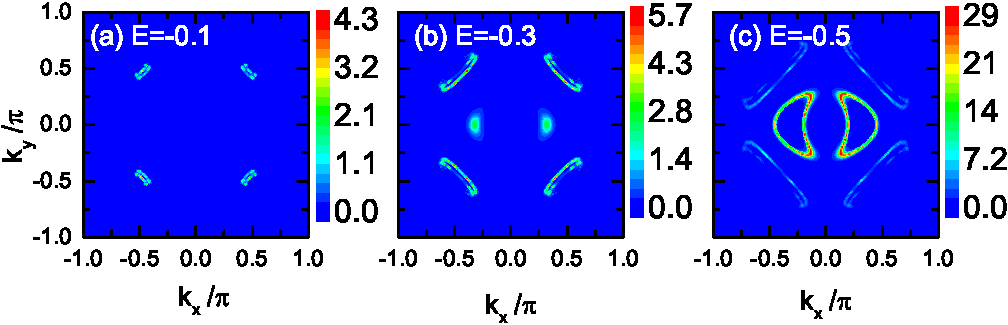
\includegraphics[scale=0.9]{pic/fig17.pdf}
\caption{2D拓扑绝缘体层谱函数强度分布。(a)$E=-0.1$,(b)$E=-0.3$,(c)$E=-0.5$}\label{fig16}
\end{figure}
计算结果显示,在低能$E=-0.1$的时候(\ref{fig16}(a)),准粒子谱中在$d$-波配对的节点位置附近形成了小的口袋状环。这个低能的谱函数的贡献正是来自于$d$-波超导层的准粒子隧穿\\cite{re59}。随着准粒子能量增加到0.3,如图\ref{fig16}(b),这个口袋的大小慢慢变大,同时在$k_y=0$的位置出也出现了另外一部分准粒子的贡献。这部分谱的权重随着能量能加变成了最大的,如图\ref{fig16}(c)所示。

 在图\ref{fig16}中有一个有趣的结果,我们发现$\mathcal{C}_4$对称性的确是被破坏了,$A(k_x,k_y)\neq A(-k_y,k_x)$,如图\ref{fig16}(b,c)所示。这个对称性被破坏的起源来自于异质结两层材料之间能带的混合,同时也与2D拓扑绝缘体中诱导出不对称的超导电子配对是有关系的。值得注意的是,在理论研究中,如果直接将一个$d$-波的超导电子配对加入到2D拓扑绝缘体的哈密顿量中,忽略两层之间的耦合,此时系统准粒子谱的$\mathcal{C}_4$对称性并未受到破坏。我们的计算结果表明,我们提出的微观模型的确可以定性的描述异质结结构的混合系统。
%==============$$==============================
\subsection{边界态计算结果及分析}
 接下来我们通过考虑一个圆柱形结构,即对于2D系统而言,一个方向是开边界的,另外一个方向是周期性边界。首先我们考虑沿$x$方向取开边界条件,沿$y$方向取周期边界条件,则$k_y$是个好量子数,在$k_y\in\left[-\pi,\pi\right]$的区间内计算哈密顿量的本征值并得到能带图,结果如图\ref{fig17}(a)所示。这里同时包括了体态与边界态的能带,在系统的两个开放边界数,能带是有能隙的。
\begin{figure}[h]
	\centering
	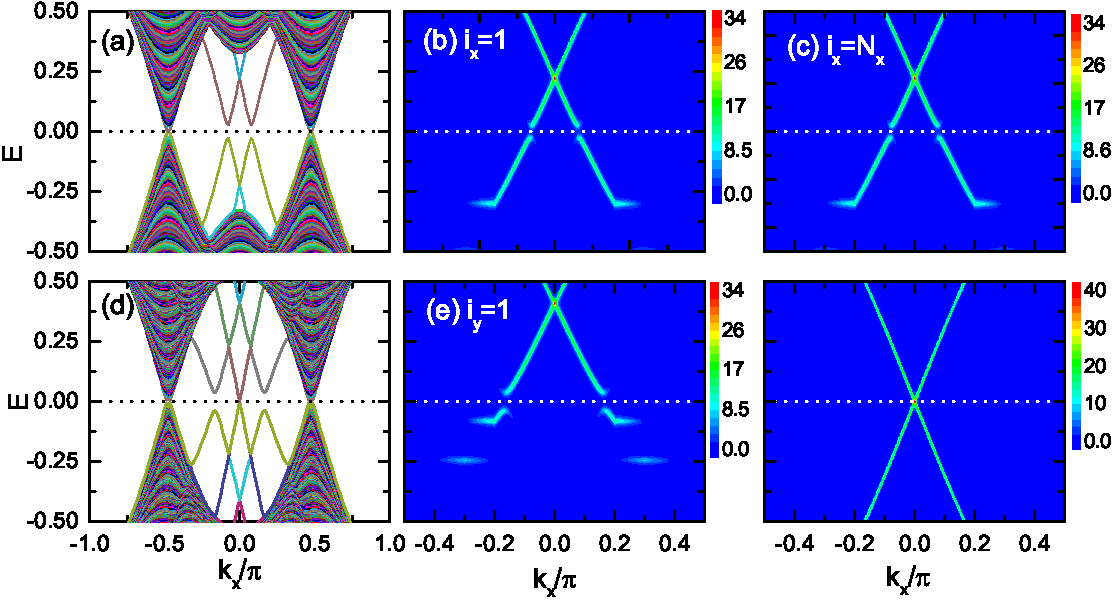
\includegraphics[scale=0.7]{pic/fig18.pdf}
	\caption{考虑圆柱形结构的数值计算结果。(a)沿$x$方向开边界时哈密顿量本征值,(b)$i_x=1$边界处的谱函数,(c)$i_x=N_x$边界处的谱函数,(d)沿$y$方向开边界时哈密顿量本征值,(b)$i_y=1$边界处的谱函数,(c)$i_y=N_y$边界处的谱函数}\label{fig17}
\end{figure}
我们同时计算了边界位置处的谱函数,如图\ref{fig17},从这里可以更加清晰的看到有能隙的边界态,着与能带计算得到的结论是完全相同的。从谱函数的结果中还可以看到,能隙的大小大约为0.05,这个被打开的能隙正是来源于近邻效应诱导的$d$-波配对项\\cite{re27,re28}。

 我们接下讨论沿$y$方向取开边界条件的边界态。此时能带图以及格点两端($i_y=1,i_y=N_y$)的的谱函数计算结果如图\ref{fig18}(d-f)所示。此时的结果与$x$方向\ref{fig17}(a-c)中的结果是不同的,这表明体系的$\mathcal{C}_4$对称性是受到破坏的。值得注意的是此时的边界态是没有能隙的,这与之前唯象的理论模型研究的结果是不同的\cite{re27,re28}。在谱函数的计算中,两个边界处的结果也是不同的。在$i_y=1$的边界上,边界态是有能隙的,能隙大小约为0.08,这个值甚至比$i_x=1$与$i_x=N_x$边界上边界态的能隙还要大。但是在$i_y=N_y$这个边界上,边界态是没有能隙的,因此对于圆柱体结构的系统,体系的非对称性是显而易见的。此时在$i_y=N_y$这个边界上存在局域的零能态,这个结果可以通过实验手段进行探测。
%============================================
\subsection{局域电子态密度结果及分析}
 现在我们通过数值的方法来研究马约拉纳拐角态。我们考虑了2D拓扑绝缘体(40$\times$40的有限大小)生长在一块更大的高温超导体上,如图\ref{fig18}(a)所示。
\begin{figure}[h]
\centering
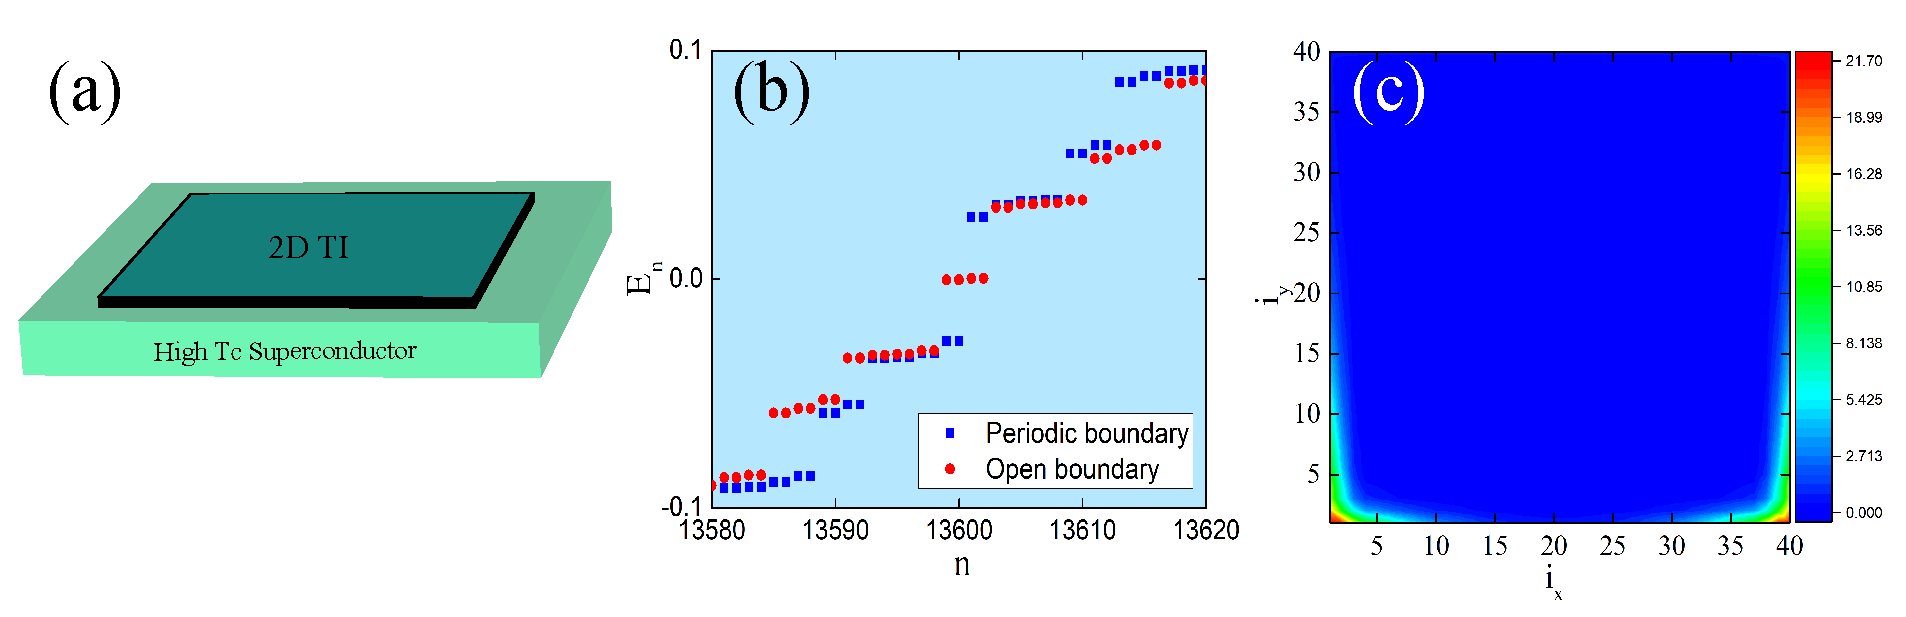
\includegraphics[scale=0.8]{pic/fig19}
\caption{(a)2D拓扑绝缘体生长在$d$-波高温超导体上,(b)实空间哈密顿量本征值(c)2D拓扑绝缘体实空间中零能态电子局域态密度}\label{fig18}
\end{figure}
首先来考虑沿$x$和$y$都取开边界条件,然后将实空间的哈密顿量矩阵对角化,得到的本征值如图\ref{fig18}(b)所示,可以看到存在四个零能本征值。当在实空间中$x$与$y$方向都取周期边界,则没有零能本征值出现。因此,这四个零能本征值是局域在边界上的,代表的是马约拉纳零能模。对于超导系统,四个零能本征值应该来源于两个零能物理的准粒子,对应着系统边界上的两对马约拉纳零能模。这两对马约拉纳零能模的空间分布可以通过计算零能本征值对应的局域电子态密度(LDOS)观测,如图\ref{fig18}(c)所示,存在两对局域在体系下边界的两个拐角处(每个拐角处存在一对)。然而在体系上边界的两个拐角处则没有零能态的存在。
%============================================
\subsection{本章总结}
 通过数值对角化矩阵的方法,我们发现了异质结耦合系统中,2D拓扑绝缘体与超导体之间耦合是比较重要的,当考虑了层间耦合时,2D拓扑绝缘体能谱的对称性会受到邻近超导层的影响,相对于唯象的将超导配对直接加入到2D拓扑绝缘体的哈密顿量中,这个微观模型可以更加正确的描述异质结系统的性质。我们同时发现不同方向上的边界态受到超导配对的影响也是不同的,这一结论从开边界时候的能带图以及边界态的谱函数计算都可以确认这一点。而从实空间LDOS的计算及第一章有效边界理论可知,此时通过近邻效应在2D拓扑绝缘体中诱导处的电子配对对称性也不再是纯$d$-波,所以在实空间中并不是每个拐角处都会出现马约拉纳束缚态。接下来我们将从动量空间以及实空间两个角度来分析这时电子配对对称性的情况。









\newpage
\section{超导序参量计算}
%\setcounter{page}{1}
%\pagestyle{plain}
接下来我们将会通过数值的方法来探索近邻效应在2D拓扑绝缘体中诱导出来的序参量的对称性,从而理解准粒子谱非对称性的起源。
\subsection{动量空间序参量计算结果}
我们在这里首先计算了拓扑绝缘体中轨道$1$在动量空间中的超导序参量$\Delta_1(\mathbf{k})$,结果如图\ref{fig19}(a)所示,丛结果中可以看到,序参量是破坏$\mathcal{C}_4$对称性的,我们将序参量$\Delta_1(\mathbf{k})$分解成单重态通道$\Delta_s$与三重态通道$\Delta_t$,$\Delta_1(\mathbf{k})=\Delta_s(\mathbf{k})+\Delta_t(\mathbf{k})$
\begin{equation}
\begin{aligned}
\Delta_s(\mathbf{k})&=\frac{1}{2}\left[\Delta_1(\mathbf{k})+\Delta_1(\mathbf{-k})\right]\\
\Delta_t(\mathbf{k})&=\frac{1}{2}\left[\Delta_1(\mathbf{k})-\Delta_1(\mathbf{-k})\right]
\end{aligned}
\end{equation}
\begin{figure}[h]
\centering
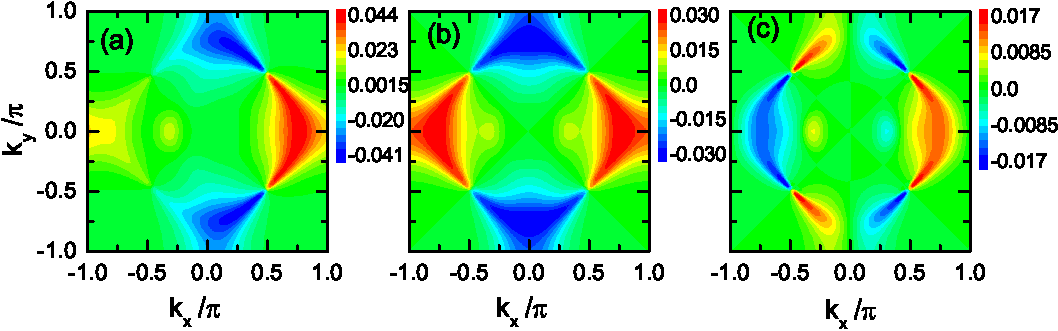
\includegraphics[scale=0.8]{pic/fig20}
\caption{(a)轨道1的超导序参量(b)轨道1单重态通道的序参量(c)轨道1三重态通道的序参量}\label{fig19}
\end{figure}
两种不同通道的序参量计算结果如图\ref{fig19}(b,c)所示,对于单重态通道$\Delta_s$,其结果与纯的$d_{x^2-y^2}$的对称性是完全相同的,但是对于三重态通道$\Delta_t$它的结果表现出了$p$-波配对的特征。所以对于2D拓扑绝缘体层轨道1,其受到超导近邻效应之后,诱导出的电子配对对称性是$(d+p)$-波,而并非只有与底层超导体相同对称性的$d$波电子配对,从数值结果中可以看到,这两种不同对称性的电子配对,其大小在相同的数量级,当同时存在相互叠加后,原来各自的对称性都会被破坏,从而形成图\ref{fig19}(a)中所示的分布,所以轨道1整体的的超导序参量$\Delta_1(\mathbf{k})$的$\mathcal{C}_4$对称性是收到破坏的,因此准粒子的谱函数的$\mathcal{C}_4$对称性同样是不存在的。同时此时超导序参量的反演对称性也是破坏的$\Delta_1(\mathbf{k})\neq\Delta_1(\mathbf{-k})$,因此在动量空间中对自旋依赖的谱函数$A_{\tau\sigma}(\mathbf{k},E)$,反演对称性也是被破坏的$A_{\tau\sigma}(\mathbf{k},E)\neq A_{\tau\sigma}(-\mathbf{k},E)$。另一方面,由于体系存在时间反演对称性,所以谱函数满足$A_{\tau\uparrow}(\mathbf{k},E)\equiv A_{\tau\downarrow}(-\mathbf{k},E)$,因此对于整个的谱函数,反演对称性是存在的,计算结果如图\ref{fig16}所示。
%============================================
\subsection{实空间序参量计算结果}
接下来,我们计算了在实空间中,同时沿$x$与$y$方向同时考虑开边界条件情况下,与格点位置依赖的轨道1对应的$d$-波超导序参量$\Delta_1(i)$,结果如图\ref{fig20}(a)所示,我们同时也单独计算了四个边界上的序参量,结果如图\ref{fig20}(b)所示。
\begin{figure}[h]
	\centering
	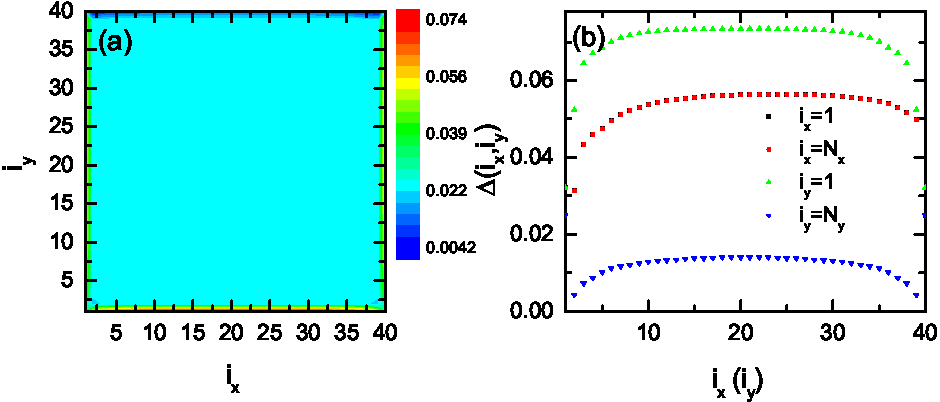
\includegraphics[scale=0.9]{pic/fig21}
	\caption{(a)2D拓扑绝缘体轨道1实空间中的$d$-波序参量(b)实空间四条边界上的$d$-波序参量分布}\label{fig20}
\end{figure}

从上面的结果中可以看到,在非边界处近邻效应诱导的$d$波电子配对是非常均匀的,但是在边界上,诱导出的电子配对与非边界处具有显著的差异。在$i_y=1$这个边界上,序参量的值相对比较大,但是在$i_y=N_y$边界上,序参量幅值是非常小的,因此在这条边上,在圆柱形结构计算的能带结果中,存在拓扑保护的无能隙的边界态,这是因为电子配对太小不足以将该边界处的准粒子无能隙边界态打开能隙,这与我们前面计算谱函数得到的结论是完全一致的。同时,对于一个开边界有限大小的体系,上边界几乎为零的$d$-波序参量并不会将此边界上的边界态打开能隙,所以也就无法和相邻边界形成质量反号的质量畴壁,这就是在这个边界相邻的拐角处无法形成束缚态的的原因。根据第一章的有效边界理论分析,正是因为$d$-波配对在不同方向上的符号相反,可以在相邻的边界上形成质量畴壁,从而在质量反号的交界处形成零能束缚态,而上边界上诱导出有效的$d$-波序参量是非常小的,并未形成能隙,所以该边界是无能隙的,不能与相邻边界形成质量畴壁,但是在下边界($i_y=1$)处,电子配作用较强,可以形成能隙,因而只能在下边界与相邻边界的拐角处形成马约拉纳拐角态,即图\ref{fig18}(c)计算结果所示。这里需要强调的是,上边界通过近邻效应诱导的超导能隙非常小这个结论是非常普适的,即使在一定范围内改变体系的化学势,结果仍然保持不变。
%============================================
\subsection{本章总结}
本章中,我们主要计算了实空间与动量空间中,在2D拓扑绝缘体中诱导出的超导配对的对称性问题。从动量空间中的计算可以看到,层间耦合导致在2D拓扑绝缘体中诱导的电子配对不仅仅具有和底层$d$-波超导体相同对称性的分量,同时也会诱导出$p$-波分量,这两种不同对称形式的配对在动量空间中混合之后就会破坏原有的$\mathcal{C}_4$对称性,因此相比较于将电子配对唯象的处理为拓扑绝缘体的本征属性,此时会对马约拉纳拐角态出现的位置有一些较大的影响。在实空间中$d$-波序参量的计算结果也表明,在不同的边界上诱导出来的能隙也是不相同的。上边界诱导的$d$-波配对幅值较小,所以无法打开边界态能隙,从而无法在上边界与其相邻边界的拐角处形成马约拉纳拐角态。这些序参量分析的结果与前面谱函数及能带计算的结果都是相互符合的。








\newpage
\section{运动方程计算结果}
本论文前面章节的数值计算,分别从谱函数以及序参量的角度研究了2D拓扑绝缘体/$d$-波超导体异质结系统中由近邻效应诱导产生超导配对,从而发现拓扑绝缘体中的$\mathcal{C}_4$对称性受到了破坏,而且马约拉纳束缚态也只是出现在系统的部分角落中。这里我们通过解析的方式来研究系统哈密顿量所对应的谱函数以及超导序参量在层间耦合作用下的具体表达形式,来分析引起对称性破坏的起源。
%\setcounter{page}{1}
%\pagestyle{plain}
\subsection{动量空间中的反常格林函数}
对于2D拓扑绝缘体,其轨道$\tau$的有效配对可以通过反常格林函数$F_\tau(\mathbf{k},\omega)=\langle\langle c^\dagger_{\mathbf{k}\tau\uparrow}|c^\dagger_{\mathbf{-k}\tau\downarrow}\rangle\rangle$来计算,它同样可以利用数值的方法进行求解,也就是推迟格林函数矩阵中的反对角线部分
\begin{equation}
F_\tau(\mathbf{k},\omega)=\sum_n\frac{u^{*}_{\tau,n}(\mathbf{k})u_{\tau+6,n}(\mathbf{k})}{\omega-E_n+i\Gamma}\label{af1}
\end{equation}
同样的,它可以解析的通过下面的运动方程来求解
\begin{equation}
\omega\langle\langle A|B\rangle\rangle=\langle\left[A,B\right]_{+}\rangle+\langle\langle\left[A,H\right]|B\rangle\rangle\label{gf11}
\end{equation}
为了求解反常格林函数,先做一些简化的记号$x_1=\langle\langle c_{{\bf k}1\uparrow}^\dagger|c_{-{\bf k}1\downarrow}^\dagger\rangle\rangle_\omega$,
$x_2 = \langle\langle c_{{\bf k}2\uparrow}^\dagger|c_{-{\bf k}1\downarrow}^\dagger\rangle\rangle_\omega$,
$x_3 = \langle\langle d_{{\bf k}\uparrow}^\dagger|c_{-{\bf k}1\downarrow}^\dagger\rangle\rangle_\omega$,
$x_4 = \langle\langle d_{-{\bf k}\downarrow}|c_{-{\bf k}1\downarrow}^\dagger\rangle\rangle_\omega$,
$x_5 = \langle\langle c_{-{\bf k}1\downarrow}|c_{-{\bf k}1\downarrow}^\dagger\rangle\rangle_\omega$,
$x_6 = \langle\langle c_{-{\bf k}2\downarrow}|c_{-{\bf k}1\downarrow}^\dagger\rangle\rangle_\omega$。对$\langle\langle\left[A,H\right]|B\rangle\rangle$重复的利用方程(\ref{gf11})就可以得到系统的反常格林函数。

异质结系统的哈密顿量为
\begin{equation}
H=H_\mathrm{TI}+H_\mathrm{SC}+H_\mathrm{I}
\end{equation}
$H_\mathrm{TI}$是正方格点上的2D拓扑绝缘体层的哈密顿量\cite{re56,re57},
\begin{equation}
	\begin{aligned}
		H_{TI} =\sum_{{\bf k}}C_{{\bf k}}^\dagger (h_\mathbf{k}\sigma_3s_0+2\lambda_{0}\sin k_x\sigma_1s_3+2\lambda_0\sin k_y\sigma_2 s_0)C_{{\bf k}},
	\end{aligned}\label{tiham}
\end{equation}
这里$h_\mathbf{k}=h_0-2t(\cos k_x+\cos k_y)$,矢量$C^\dagger_{\bf k}$ 可以表示为$C^\dagger_{\bf k}=(c^\dagger_{{\bf k}1\uparrow},c^\dagger_{{\bf k}2\uparrow},c^\dagger_{{\bf k}1\downarrow},c^\dagger_{{\bf k}2\downarrow})$,这里下表$1,2$和$\uparrow,\downarrow$分别代表的是轨道与自旋索引。$s_i$与$\sigma_i$分别代表的是自旋空间和轨道空间的单位矩阵($i=0$)或者泡里矩阵($i=1,2,3$)。

$H_\mathrm{SC}$描述一个$d$-波超导体
\begin{equation}
	H_{SC}=\sum_{{\bf k}\sigma}\varepsilon_{\bf k}d^\dagger_{{\bf k}\sigma}d_{{\bf k}\sigma}+\sum_{{\bf k}}\Delta_{\bf k}(d^\dagger_{{\bf k}\uparrow}d^\dagger_{{-\bf k}\downarrow}+h.c.),
\end{equation}
这里 $\varepsilon_{\bf k}=-2t(\cos k_x+\cos k_y)-\mu$, 动量空间中的超导配对为 $\Delta_{\bf k}=2\Delta_0 (\cos k_x-\cos k_y)$.

$H_\mathrm{I}$描述的是超导层与2D拓扑绝缘体层之间的单粒子跃迁项
\begin{equation}
	H_{I}=-t_\perp \sum_{{\bf k}\tau\sigma}(c_{{\bf k}\tau\sigma}^\dagger d_{{\bf k}\sigma}+h.c.).
\end{equation}
我们可以得到下面的方程组
\begin{subequations}
	\begin{eqnarray}
		ax_1&=&fx_2+t_\perp x_3
		\\
		bx_2&=&ex_1+t_\perp x_3
		\\
		cx_3&=&gx_4+t_\perp (x_1+x_2)
		\\
		dx_4&=&gx_3-t_\perp (x_5+x_6)
		\\
		bx_5&=&1-fx_6-t_\perp x_4
		\\
		ax_6&=&-ex_5-t_\perp x_4,\label{eom2}
	\end{eqnarray}
\end{subequations}
这里 $a=\omega-h_{\bf k}$, $b=\omega + h_{\bf k}$, $c=\omega-\varepsilon_{\bf k}$,
$d=\omega+\varepsilon_{\bf k}$, $e=2\lambda_0\sin(k_x)-2i \lambda_0\sin(k_y)$, $f=2\lambda_0\sin(k_x) + 2i\lambda_0\sin(k_y)$,
并且令 $g = \Delta_{\bf k}$.

最后通过求解方程组(\ref{eom2})就可以得到轨道1的反常格林函数
\begin{equation}
\langle\langle c_{{\bf k}1\uparrow}^\dagger|c_{-{\bf k}1\downarrow}^\dagger\rangle\rangle=\frac{\Delta_{\bf k} t_\perp ^2 (a-e) (b+f)}{\Omega}=\frac{\Delta_{\bf k}t_\perp^2(C_{even}+C_{odd})}{\Omega},\label{anlyagf}
\end{equation}
这里的符号简记为 $\Omega=-\left(c d-g^2\right) (a b-e f)^2+t_\perp ^2 (a b-e f) [a (c+d)+b (c+d)-(c-d) (e+f)]-t_\perp ^4 (a+b-e-f) (a+b+e+f)$, $C_{even}=\omega^2-h^2_{\bf{k}}-4\lambda_0[\sin^2(k_x)+\sin^2(k_y)]$, $C_{odd}=4\omega\lambda i\sin(k_y)-4h_{\mathbf{k}}\lambda_0\sin(k_x)$。

从这个公式(\ref{anlyagf})中我们可以看到,反常格林函数的确同时包括了奇宇称和偶宇称部分,而且$\mathcal{C}_4$对称性也是被破坏的。通过进行解析延拓($\omega\rightarrow\omega+i\Gamma$),我们就可以得到推迟反常格林函数$F_\tau(\mathbf{k},\omega)$。方程(\ref{anlyagf})的数值计算结果与通过直接对角化哈密顿量矩阵计算反常格林函数(\ref{af1})得到的结果是完全相同的。

接下来我们对反常格林函数中的$\omega$积分,从而得到只与动量$\mathbf{k}$依赖的函数$F_\tau(\mathbf{k})$来描述体系的有效电子配对
\begin{equation}
F_\tau({\bf k})=-\int_{-\infty}^0\mathrm{Im}F_\tau({\bf k},\omega)d\omega.
\end{equation}

利用和前面相同的方式,我们将动量依赖的反常格林函数分解为单重态通道$F^s_\tau(\mathbf{k})$与三重态通道$F^t_\tau(\mathbf{k})$
\begin{equation}
\begin{aligned}
F_s({\bf k})&=1/2[F_1({\bf k})+F_1(-{\bf k})]\\
F_t({\bf k})&=1/2[F_1({\bf k})-F_1(-{\bf k})]
\end{aligned}
\end{equation}
反常格林函数$F_1(\mathbf{k})$以及$F_s({\bf k}),F_t({\bf k})$在动量空间中的结果如图\ref{fig21}(a-c)所示,如结果所示,我们从解析方式求解得到的结果与我们在第四章通过数值方法得到的结果图\ref{fig19}(a-c)在定性上是完全一致的。
\begin{figure}[h]
\centering
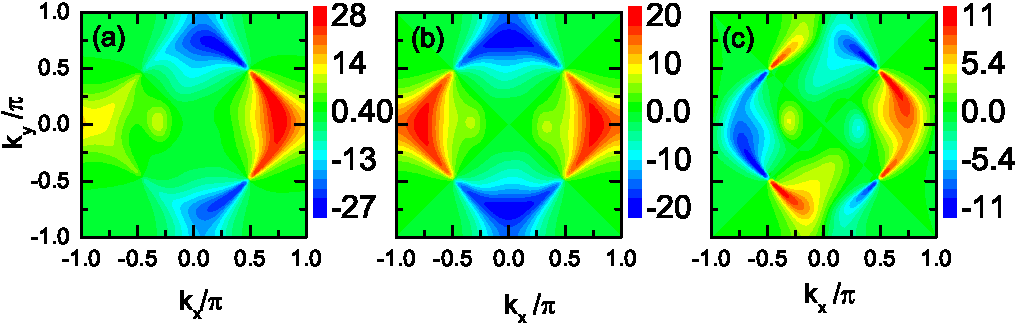
\includegraphics[scale=0.8]{pic/fig22}
\caption{(a)反常格林函数计算轨道1的超导序参量(b)轨道1单重态通道的序参量(c)轨道1三重态通道的序参量}\label{fig21}
\end{figure}
%============================================
\subsection{系统边界处的反常格林函数}
接下来我们利用运动方程来计算系统边界上的反常格林函数,首先从描述2D拓扑绝缘体在圆柱体结构下的哈密顿量开始。通常我们可以将哈密顿量进行对角化$H=\sum_n\epsilon_n\gamma^\dagger\gamma$。对2D拓扑绝缘体而言,它的体态始终存在能隙,而低能($\epsilon_n\rightarrow 0$)准粒子激发通常出现在系统的边界上。准粒子算符$\gamma^\dagger$与原来的粒子算符$c_{k_x,\tau\sigma}$之间是通过能量本征值$\epsilon_n$对应的本征矢量联系起来的,利用这个关系我们就可以得到2D拓扑绝缘体在边界上的哈密顿量。在$i_y=1$这个边界上,有效的哈密顿量可以近似的表示为
\begin{equation}
H_{(i_y=1)}=-\sum_{\sigma,\tau}\sigma k c_{k\tau\sigma}^\dagger c_{k\tau\sigma}-\sum_\sigma(\sigma k c_{k1\sigma}^\dagger c_{k2\sigma}+h.c),\label{iy1}
\end{equation}
这里将$k_x$简记为$k$,$\sigma$取$\pm$代表着自旋向上与自旋向下。

高温超导体层的哈密顿量为
\begin{equation}
H_{SC}=\sum_\sigma\epsilon_{k} d_{k\sigma}^\dagger d_{k\sigma}+(\Delta_{ k} d_{k\uparrow}^\dagger d_{-k\downarrow}^\dagger+h.c).
\end{equation}

两层之间的耦合为
\begin{equation}
H_I=-\sum_{\sigma,\tau}(t_\perp c_{k\tau\sigma}^\dagger d_{k\sigma}+h.c).
\end{equation}

为了计算方便,先定义下面的六个格林函数元素
$x_1=\langle\langle c_{k1\uparrow}^\dagger|c_{-k1\downarrow}^\dagger$$\rangle$$\rangle_\omega$, $x_2=\langle\langle c_{k2\uparrow}^\dagger|c_{-k1\downarrow}^\dagger$$\rangle$$\rangle_\omega$, $x_3=\langle\langle d_{k\uparrow}^\dagger|c_{-k1\downarrow}^\dagger\rangle\rangle_\omega$, $x_4=\langle\langle d_{-k\downarrow}|c_{-k1\downarrow}^\dagger\rangle\rangle_\omega$, $x_5=\langle\langle c_{-k1\downarrow}|c_{-k1\downarrow}^\dagger\rangle\rangle_\omega$, $x_6=\langle\langle c_{-k2\downarrow}|c_{-k1\downarrow}^\dagger\rangle\rangle_\omega$,根据运动方程(\ref{gf11})可以得到下面的方程组
\begin{subequations}
	\begin{eqnarray}
	(\omega+k)x_1&=&-kx_2-tx_3\\
	(\omega+k)x_2&=&-kx_1-tx_3\\
	(\omega-\epsilon_{k})x_3&=&-t(x_1+x_2)+\Delta_{k} x_4\\
	(\omega+\epsilon_{k})x_4&=&t(x_5+x_6)+\Delta_{k} x_3\\
	(\omega+k)x_5&=&1-k x_6+tx4\\
	(\omega+k)x_6&=&-k x_5+tx_4
	\end{eqnarray}\label{agf2}
\end{subequations}
通过求解方程组(\ref{agf2})就可以得到边界上轨道1的反常格林函数
\begin{equation}
F_{(i_y=1)}=\frac{\Delta_{k} t_\perp^2}{\Delta_k^2(2k+\omega)^2+\epsilon_k^2(2k+\omega)^2-[-2t_\perp^2+\omega(2k+\omega)]^2}.
\end{equation}

其他边界上的有效哈密顿量同样可以得到
\begin{equation}
H_{(i_y=N_y)}=\sum_{\sigma,\tau}\sigma k c_{k\tau\sigma}^\dagger c_{k\tau\sigma}-\sum_\sigma(\sigma k c_{k1\sigma}^\dagger c_{k2\sigma}+h.c),\label{iyn}
\end{equation}

\begin{equation}
H_{(i_x=1)}=\sum_{\sigma,\tau}\sigma k c_{k\tau\sigma}^\dagger c_{k\tau\sigma}-\sum_\sigma(i k c_{k1\sigma}^\dagger c_{k2\sigma}+h.c),\label{ix1}
\end{equation}

\begin{equation}
H_{(i_x=N_x)}=-\sum_{\sigma,\tau}\sigma k c_{k\tau\sigma}^\dagger c_{k\tau\sigma}-\sum_\sigma(i k c_{k1\sigma}^\dagger c_{k2\sigma}+h.c),\label{ixn}
\end{equation}
利用相似的求解方法,可以得到这些边界上轨道1的反常格林函数为
\begin{equation}
F_{(i_y=N_y)}=\frac{\Delta_k t_\perp^2}{(\Delta_k^2+\epsilon_k^2)\omega^2-(-2t_\perp^2+\omega^2)^2}\label{cyyL}.
\end{equation}

\begin{equation}
\begin{aligned}
F_{(i_x=1)}&=-\frac{\Delta_k  t_\perp^2 \left(2 k^2+2 k \omega +\omega ^2\right)}{\Omega}\\
\Omega&=4 k^2 \left[t_\perp^4-\omega ^2 \left(\Delta_k ^2+2 t_\perp^2+\epsilon_k ^2\right)+\omega ^4\right]+4 k \omega  \left[2 t_\perp^4-\omega ^2 \left(\Delta_k ^2+3 t_\perp^2+\epsilon_k ^2\right)+\omega ^4\right]\\
&+4 t_\perp^4 \omega ^2-\omega ^4 \left(\Delta_k ^2+4 t_\perp^2+\epsilon_k ^2\right)+\omega ^6\label{cyxL}
\end{aligned}
\end{equation}
	
\begin{equation}
F_{(i_x=N_x)}=-\frac{\Delta_k  t_\perp^2 \left(2 k^2-2 k \omega +\omega ^2\right)}{\Omega}\label{cyx1}
\end{equation}

在低能量下,对这些反常格林函数做低阶泰勒展开
\begin{equation}
\begin{aligned}
F_{(i_y=1)}\approx&-\frac{\Delta_k  t_\perp^2}{-\Delta_k ^2 \omega ^2+4 t_\perp^4-4 t_\perp^2 \omega ^2+\omega ^4-\omega ^2 \epsilon_k ^2}-\frac{4  \left[\Delta_k  t_\perp^2 \left(\Delta_k ^2 \omega +2 t_\perp^2 \omega -\omega ^3+\omega  \epsilon_k ^2\right)\right]}{\left(-\Delta_k ^2 \omega ^2+4 t_\perp^4-4 t_\perp^2 \omega ^2+\omega ^4-\omega ^2 \epsilon_k ^2\right)^2}k\\
&+\frac{4 \Delta_k   t_\perp^2 \left[-4 t_\perp^4 \left(\Delta_k ^2+\epsilon_k ^2\right)+6 \omega ^4 \left(\Delta_k ^2+2 t_\perp^2+\epsilon_k ^2\right)-3 \omega ^2 \left(\Delta_k ^2+2 t_\perp^2+\epsilon_k ^2\right)^2-3 \omega ^6\right]}{\left(4 t_\perp^4-\omega ^2 \left(\Delta_k ^2+4 t_\perp^2+\epsilon_k ^2\right)+\omega ^4\right)^3}k^2,
\end{aligned}
\end{equation}
\begin{equation}
F_{(i_y=N_y)}=-\frac{\Delta_k  t_\perp^2}{-\Delta_k ^2 \omega ^2+4 t_\perp^4-4 t_\perp^2 \omega ^2+\omega ^4-\omega ^2 \epsilon_k ^2},
\end{equation}


\begin{small}
\begin{equation}
\begin{aligned}
&F_{(i_x=1)}\approx-\frac{\Delta_k  t_\perp^2}{-\Delta_k ^2 \omega ^2+4 t_\perp^4-4 t_\perp^2 \omega ^2+\omega ^4-\omega ^2 \epsilon_k ^2}+\frac{2 \Delta_k   t_\perp^2 \omega  \left(\Delta_k ^2+2 t_\perp^2-\omega ^2+\epsilon_k ^2\right)}{\left(-\Delta_k ^2 \omega ^2+4 t_\perp^4-4 t_\perp^2 \omega ^2+\omega ^4-\omega ^2 \epsilon_k ^2\right)^2}k\\
&+\frac{2 \Delta_k   t_\perp^2 \left[-3 \omega ^4 \left(\Delta_k ^2-\omega ^2+\epsilon_k ^2\right)^2-8 t_\perp^8+24 t_\perp^6 \omega ^2+6 t_\perp^4 \omega ^2 \left(\Delta_k ^2-5 \omega ^2+\epsilon_k ^2\right)-16 t_\perp^2 \omega ^4 \left(\Delta_k ^2-\omega ^2+\epsilon_k ^2\right)\right]}{\omega ^2 \left(4 t_\perp^4-\omega ^2 \left(\Delta_k ^2+4 t_\perp^2+\epsilon_k ^2\right)+\omega ^4\right)^3}k^2,
\end{aligned}
\end{equation}
\end{small}
\begin{small}
\begin{equation}
\begin{aligned}
&F_{(i_x=N_x)}\approx-\frac{\Delta_k  t_\perp^2}{-\Delta_k ^2 \omega ^2+4 t_\perp^4-4 t_\perp^2 \omega ^2+\omega ^4-\omega ^2 \epsilon_k ^2}-\frac{2  \left(\Delta_k  t_\perp^2 \omega  \left(\Delta_k ^2+2 t_\perp^2-\omega ^2+\epsilon_k ^2\right)\right)}{\left(-\Delta_k ^2 \omega ^2+4 t_\perp^4-4 t_\perp^2 \omega ^2+\omega ^4-\omega ^2 \epsilon_k ^2\right)^2}k\\
&+\frac{2 \Delta_k   t_\perp^2 \left[-3 \omega ^4 \left(\Delta_k ^2-\omega ^2+\epsilon_k ^2\right)^2-8 t_\perp^8+24 t_\perp^6 \omega ^2+6 t_\perp^4 \omega ^2 \left(\Delta_k ^2-5 \omega ^2+\epsilon_k ^2\right)-16 t_\perp^2 \omega ^4 \left(\Delta_k ^2-\omega ^2+\epsilon_k ^2\right)\right]}{\omega ^2 \left(4 t_\perp^4-\omega ^2 \left(\Delta_k ^2+4 t_\perp^2+\epsilon_k ^2\right)+\omega ^4\right)^3}k^2.
\end{aligned}
\end{equation}
\end{small}
这里的$k^2$项是由无能隙的边界态贡献的有效单重态的配对,在$i_x=1$与$i_x=N_x$边界上,反常格林函数在单重态的贡献是完全相同的。然而在$i_y=N_y$边界上,来自轨道内的耦合贡献与轨道间的耦合贡献相互抵消,所以在这个边界上电子有效配对的量值非常小。

上面的结果也可以通过定性的方式进行理解,如公式(\ref{iy1}),(\ref{iyn}),(\ref{ix1}),(\ref{ixn})所示,边界有效哈密顿量同时包含了轨道间以及轨道内的跃迁项,当与超导体进行耦合时,这两部分都会对边界上的有效电子配对产生贡献。轨道内的跃迁应该与2D拓扑绝缘体螺旋边界态的性质相同,在两个边界上会发生反号。而且从公式(\ref{tiham})中可以看出在$i_y$的边界上,轨道间的跃迁是个实常数,在$i_x$边界上则是虚常数。结果就是在$i_y=N_y$边界上,轨道间的跃迁常数与轨道内的跃迁常数实相反的,它们之间会相互抵消,从而在这个边界上形成的电子配对会非常小。然而在$i_y=1$边界上,这个项的贡献是相同的,会叠加起来,从而在这个边界上的电子配对强度会变得比较大。对于$i_x=1$或者$i_x=N_x$边界,轨道间的跃迁常数是虚常数,在这个边界上同样可以诱导出有效的$d$-波电子配对,但是其大小会小于$i_y=1$边界上。
%============================================
\subsection{本章总结}
在本章中,通过运动方程的方法,我们计算了体态电子的反常格林函数,得到了与数值计算相同的结果,并发现的确会同时存在奇宇称和偶宇称两种不同通道的电子配对。通过近邻效应在拓扑绝缘体中会同时诱导处$d$-波电子配对和$p$-波电子配对。而$p$-波配对则主要是来源于拓扑绝缘体中自旋轨道耦合的贡献。

接下来我们从边界有效的哈密顿量出发,利用运动方程对每个边界上的反常格林函数进行了计算,结果发现在不同边界上诱导出的电子配对形式是不相同的,特别是在$i_y=N_y$这个边界上,因为自旋轨道耦合的作用,这条边界上的电子配对会非常小,从而在这个边界上2D拓扑绝缘体的螺旋边界态始终未能打开能隙,而其它三个边界上都会存在可观大小的$d$-波电子配对。这也成功的解释了为何在体系中,与上边界相邻的位置无法产生马约拉纳拐角态。













\newpage
\section{总结与展望}
高阶拓扑超导体与普通的一阶拓扑超导体具有不同的性质,其马约拉纳束缚态会出现在比系统维度低两维甚至三维的边界上。第一章主要介绍了拓扑绝缘体,超导体,以及高阶拓扑超导体的基本概念,并从低能边界态理论出发介绍了在2D系统的拐角处,高阶拓扑超导体产生的机制。科研人员利用2D拓扑绝缘体与各向异性配对的$d$-波超导体构成的异质结来实现高阶拓扑超导体,从而在系统的角落中存在马约拉纳拐角态。同时研究人员也研究了利用常规的$s$-波超导体与一个面内的Zeeman场,当与2D拓扑绝缘体形成异质结系统的时候,也可以在拐角处形成马约拉纳拐角态,但此时面内的Zeeman场破坏了时间反演对称性,所以在每个拐角处只存在一个马约拉纳拐角态。随后我们介绍了在通过异质结结构研究一阶拓扑超导体的时候,层间的耦合会对诱导出的电子配对对称性存在一定影响,研究人员发现除了超导本来的配对形式,因为晶体结构之间的不匹配,还会存在其他形式的电子配对会在近邻层产生,这种形况下形成的其实是混合类型的超导配对。在第二章,基于异质结结构的复杂性,在唯象模型研究的基础上,我们给出了一个研究高阶拓扑超导体的微观模型,主要考虑了超导体与2D拓扑绝缘体之间的耦合作用,并介绍了具体的研究方法。第三章我们主要研究了微观模型的能带以及边界态谱函数,发现体系的$\mathcal{C}_4$对称性破缺,而且特定位置的边界态并没有因为近邻效应的存在而打开能隙,并通过计算零能态的局域电子密度,发现在实空间中,未打开能隙的边界上确实在其拐角处不存在马约拉纳拐角态。第四章中我们计算了动量空间中以及实空间中的序参量,进一步确定了通过近邻效应诱导的电子配对的对称性,发现通过近邻效应诱导的电子配对同时包含了单重态与三重态两种成分。对实空间$d$-波电子配对的计算也发现了在体系的上边界,通过近邻效应诱导出的电子配对是很小的,所以这再次验证了我们之前关于能带以及谱函数的计算。在第五章中,我们利用运动方程的方法,求解了单个轨道的反常格林函数,即就是电子配对,发现此时可以将电子的配对分成奇宇称通道和偶宇称通道,通过对费米面以下的积分,计算得到的电子配对结果与我们利用数值对角化矩阵计算超导序参量的结果是完全相同的。我们同时也利用准粒子的边界哈密顿量计算了系统边界上的反常格林函数,发现在$i_y=N_y$这个边界上,电子配对的贡献是非常小的。

综上所述,我们从数值以及解析两种不同的方式,利用微观模型研究了2D拓扑绝缘体与$d$-波超导体形成的异质结中,我们发现马约拉纳拐角态只会出现在部分角落中,而对于唯象模型研究则显示系统的所有角落中都会出现马约拉纳拐角态。

我们的计算表明,这种不一致主要来源于近邻效应在2D拓扑绝缘体中诱导出来的是$d+p$-波的电子配对,正是因为这种配对破坏了$\mathcal{C}_4$对称性,而且不同边界上电子配对大小也是不同的,所以只会在部分角落中才会出现马约拉纳拐角态,这对之后实验上利用异质结结构探索高阶拓扑中的马约拉纳拐角态具有一定的价值,也为利用高阶拓扑超导体中利用马约拉纳拐角态实现拓扑量子计算有一定的应用价值。





%=================================================
\newpage
\addcontentsline{toc}{section}{参考文献} %向目录中添加条目,以章的名义
%\bibliographystyle{IEEEtran} % 参考文献样式
%\bibliographystyle{elsarticle-num} % 大致可以
%\bibliography{ref}%加入参考文献
\bibliographystyle{bstutf8}
\bibliography{ref2}%加入参考文献

%==============================================
\newpage
\addcontentsline{toc}{section}{致谢} %向目录中添加条目,以章的名义
\begin{center}
	\zihao{3}\bf 致谢
\end{center}

这里是致谢





  % 致谢
\addcontentsline{toc}{section}{作者攻读学位期间发表的学术论文目录} %向目录中添加条目,以章的名义
\newpage
\newpage
\centering{\zihao{3}\bf 作者攻读学位期间发表的学术论文目录}
\flushleft{\zihao{4}\bf 发表的学术论文}

\begin{itemize}
	\item {\bf Yu-Xuan Li} and Tao Zhou$^{*}$,Rotational symmetry breaking and partial Majorana corner states in a heterostructure
	based on high-T$_c$ superconductors,Physical Review B 103, 024517 (2021)
\end{itemize}

\begin{enumerate}
	\item {\bf Yu-Xuan Li} and Tao Zhou$^{*}$,Rotational symmetry breaking and partial Majorana corner states in a heterostructure
	based on high-T$_c$ superconductors,Physical Review B 103, 024517 (2021)
\end{enumerate}  % 论文发表
\end{document}
